\documentclass[11pt,a4paper]{article}
\usepackage[english]{babel}
\usepackage[utf8]{inputenc}
\usepackage[T1]{fontenc}
\usepackage{lmodern}
\usepackage{geometry}
\geometry{margin=2.5cm}
\usepackage{graphicx}
\usepackage{amsmath, amssymb, amsthm}
\usepackage{algorithm}
\usepackage{algpseudocode}
\usepackage{booktabs}
\usepackage{multirow}
\usepackage{array}
\usepackage{pdflscape}
\usepackage[authoryear,round]{natbib}
\usepackage{xcolor}
\usepackage{hyperref}
\hypersetup{colorlinks=true,linkcolor=blue!50!black,citecolor=blue!50!black,urlcolor=blue!50!black}
\newtheorem{proposition}{Proposition}
\newtheorem{corollary}{Corollary}
\emergencystretch=1.5em

% Every number in the text, tables and figures is generated by analyze.py
% from the run-level logs; do not edit numbers.tex or the tables by hand.
\newcommand{\mADiff}{0.071}
\newcommand{\mAHi}{0.103}
\newcommand{\mAL}{3}
\newcommand{\mALo}{0.045}
\newcommand{\mAP}{1.6\times10^{-10}}
\newcommand{\mAPairs}{57}
\newcommand{\mARatio}{2.4}
\newcommand{\mARuns}{465}
\newcommand{\mAT}{18}
\newcommand{\mAW}{36}
\newcommand{\mAbpxAll}{22}
\newcommand{\mAbpxFound}{33}
\newcommand{\mAbpxGap}{0.050}
\newcommand{\mAbpxHit}{54.4}
\newcommand{\mAbpxMax}{0.480}
\newcommand{\mAllExact}{yes}
\newcommand{\mAvnsAll}{18}
\newcommand{\mAvnsFound}{25}
\newcommand{\mAvnsGap}{0.121}
\newcommand{\mAvnsHit}{38.7}
\newcommand{\mAvnsMax}{0.717}
\newcommand{\mBpxSharePct}{22.9}
\newcommand{\mCompsHi}{7.3}
\newcommand{\mCompsLo}{0.4}
\newcommand{\mCompsMid}{2.4}
\newcommand{\mCompsTop}{18.8}
\newcommand{\mDDiff}{0.024}
\newcommand{\mDHi}{0.037}
\newcommand{\mDL}{1}
\newcommand{\mDLo}{0.012}
\newcommand{\mDP}{0.0024}
\newcommand{\mDPairs}{19}
\newcommand{\mDRatio}{2.8}
\newcommand{\mDRuns}{140}
\newcommand{\mDT}{7}
\newcommand{\mDW}{11}
\newcommand{\mDbpxAll}{11}
\newcommand{\mDbpxFound}{14}
\newcommand{\mDbpxGap}{0.013}
\newcommand{\mDbpxHit}{76.4}
\newcommand{\mDbpxMax}{0.066}
\newcommand{\mDvnsAll}{7}
\newcommand{\mDvnsFound}{13}
\newcommand{\mDvnsGap}{0.037}
\newcommand{\mDvnsHit}{47.9}
\newcommand{\mDvnsMax}{0.112}
\newcommand{\mExGain}{$-445$}
\newcommand{\mExNC}{4}
\newcommand{\mExQ}{12}
\newcommand{\mExZC}{493776}
\newcommand{\mExZS}{494221}
\newcommand{\mExZT}{494561}
\newcommand{\mFDiff}{0.003}
\newcommand{\mFHi}{0.008}
\newcommand{\mFL}{6}
\newcommand{\mFLo}{0.001}
\newcommand{\mFP}{0.277}
\newcommand{\mFPairs}{27}
\newcommand{\mFRatio}{1.1}
\newcommand{\mFRuns}{270}
\newcommand{\mFT}{12}
\newcommand{\mFW}{9}
\newcommand{\mFbpxAll}{11}
\newcommand{\mFbpxFound}{17}
\newcommand{\mFbpxGap}{0.048}
\newcommand{\mFbpxHit}{52.2}
\newcommand{\mFbpxMax}{0.441}
\newcommand{\mFbpxfAll}{11}
\newcommand{\mFbpxfFound}{17}
\newcommand{\mFbpxfGap}{0.045}
\newcommand{\mFbpxfHit}{51.1}
\newcommand{\mFbpxfMax}{0.455}
\newcommand{\mFlbpxGap}{0.1436}
\newcommand{\mFlvnsGap}{0.2392}
\newcommand{\mGapbpxHi}{0.0449}
\newcommand{\mGapbpxLo}{0.0000}
\newcommand{\mGapbpxMid}{0.0200}
\newcommand{\mGapbpxTop}{0.1368}
\newcommand{\mGapvnsHi}{0.1675}
\newcommand{\mGapvnsLo}{0.0000}
\newcommand{\mGapvnsMid}{0.0504}
\newcommand{\mGapvnsTop}{0.2746}
\newcommand{\mHfourP}{0.277}
\newcommand{\mHfourPadj}{0.500}
\newcommand{\mHoneP}{1.0\times10^{-7}}
\newcommand{\mHonePadj}{4.2\times10^{-7}}
\newcommand{\mHthreeP}{3.1\times10^{-5}}
\newcommand{\mHthreePadj}{9.2\times10^{-5}}
\newcommand{\mHtwoP}{0.250}
\newcommand{\mHtwoPadj}{0.500}
\newcommand{\mInstN}{7}
\newcommand{\mInstP}{0.016}
\newcommand{\mInstW}{7}
\newcommand{\mIterRatio}{1.14}
\newcommand{\mIterRatioHi}{1.26}
\newcommand{\mIterRatioLo}{1.00}
\newcommand{\mIterRatioMid}{1.08}
\newcommand{\mIterRatioTop}{1.22}
\newcommand{\mLL}{1}
\newcommand{\mLLostList}{d2103 with $p=100$}
\newcommand{\mLP}{0.0004}
\newcommand{\mLPairs}{15}
\newcommand{\mLRatio}{5.4}
\newcommand{\mLT}{1}
\newcommand{\mLW}{13}
\newcommand{\mLbpxGap}{0.0339}
\newcommand{\mLbpxHit}{46.7}
\newcommand{\mLsRatio}{3.2}
\newcommand{\mLsbpxGap}{0.0842}
\newcommand{\mLsbpxHit}{24.0}
\newcommand{\mLsvnsGap}{0.2689}
\newcommand{\mLsvnsHit}{6.7}
\newcommand{\mLvnsGap}{0.1846}
\newcommand{\mLvnsHit}{12.0}
\newcommand{\mNImproved}{1}
\newcommand{\mNPairsHi}{14}
\newcommand{\mNPairsLo}{15}
\newcommand{\mNPairsMid}{14}
\newcommand{\mNPairsTop}{14}
\newcommand{\mNRefReached}{37}
\newcommand{\mNTspPairs}{57}
\newcommand{\mODiff}{0.000}
\newcommand{\mOHi}{0.001}
\newcommand{\mOL}{0}
\newcommand{\mOLo}{0.000}
\newcommand{\mOP}{0.250}
\newcommand{\mOPairs}{40}
\newcommand{\mORuns}{1200}
\newcommand{\mOT}{37}
\newcommand{\mOW}{3}
\newcommand{\mObpxAll}{40}
\newcommand{\mObpxFound}{40}
\newcommand{\mObpxGap}{0.000}
\newcommand{\mObpxHit}{100.0}
\newcommand{\mObpxHits}{1200}
\newcommand{\mObpxMax}{0.000}
\newcommand{\mObpxMinHits}{30}
\newcommand{\mObpxWorst}{0.000}
\newcommand{\mOhardPairs}{13}
\newcommand{\mOhardbpxHit}{100.0}
\newcommand{\mOhardvnsHit}{99.0}
\newcommand{\mOldhgaGap}{0.021}
\newcommand{\mOldhgaHit}{79.5}
\newcommand{\mOldvnsGap}{0.003}
\newcommand{\mOldvnsHit}{93.8}
\newcommand{\mOvnsAll}{37}
\newcommand{\mOvnsFound}{40}
\newcommand{\mOvnsGap}{0.000}
\newcommand{\mOvnsHit}{99.1}
\newcommand{\mOvnsHits}{1189}
\newcommand{\mOvnsMax}{0.006}
\newcommand{\mOvnsMinHits}{23}
\newcommand{\mOvnsWorst}{0.058}
\newcommand{\mPxCalls}{1{,}787{,}131}
\newcommand{\mPxTakePct}{0.7}
\newcommand{\mRefSentence}{For d2103 with $p=50$ our runs found a better value than the published one (302190 against 302221; algorithms that improved on the published value: VNS, VNS$_{20}$, MK-BPX, MK-BPX$_{4}$), and the better value is used as reference.}
\newcommand{\mRlbpxGap}{0.0695}
\newcommand{\mRlvnsGap}{0.1062}
\newcommand{\mSDiff}{0.068}
\newcommand{\mSHi}{0.109}
\newcommand{\mSL}{0}
\newcommand{\mSLo}{0.034}
\newcommand{\mSP}{3.1\times10^{-5}}
\newcommand{\mSPairs}{27}
\newcommand{\mSRatio}{2.4}
\newcommand{\mSRuns}{270}
\newcommand{\mST}{11}
\newcommand{\mSW}{16}
\newcommand{\mSbpxAll}{11}
\newcommand{\mSbpxFound}{17}
\newcommand{\mSbpxGap}{0.048}
\newcommand{\mSbpxHit}{52.2}
\newcommand{\mSbpxMax}{0.441}
\newcommand{\mShareHi}{25.7}
\newcommand{\mShareLo}{4.1}
\newcommand{\mShareMid}{22.2}
\newcommand{\mShareTop}{21.8}
\newcommand{\mSpBigMax}{44}
\newcommand{\mSpBigMin}{4.9}
\newcommand{\mSpCases}{21}
\newcommand{\mSpMax}{44}
\newcommand{\mSpMin}{1.8}
\newcommand{\mSvnstAll}{11}
\newcommand{\mSvnstFound}{14}
\newcommand{\mSvnstGap}{0.116}
\newcommand{\mSvnstHit}{43.3}
\newcommand{\mSvnstMax}{0.657}
\newcommand{\mTBothAll}{11}
\newcommand{\mTDiff}{0.095}
\newcommand{\mTHi}{0.139}
\newcommand{\mTInstW}{5}
\newcommand{\mTL}{2}
\newcommand{\mTLo}{0.057}
\newcommand{\mTLostList}{d2103 with $p=100$, rl5934 with $p=300$}
\newcommand{\mTP}{1.0\times10^{-7}}
\newcommand{\mTPairs}{38}
\newcommand{\mTRatio}{2.4}
\newcommand{\mTRuns}{325}
\newcommand{\mTT}{11}
\newcommand{\mTW}{25}
\newcommand{\mTakeHi}{1.0}
\newcommand{\mTakeLo}{0.0}
\newcommand{\mTakeMid}{0.8}
\newcommand{\mTakeTop}{0.8}
\newcommand{\mTbigPairs}{25}
\newcommand{\mTbigbpxGap}{0.1019}
\newcommand{\mTbigbpxHit}{18.5}
\newcommand{\mTbigvnsGap}{0.2451}
\newcommand{\mTbigvnsHit}{5.0}
\newcommand{\mTbpxAll}{11}
\newcommand{\mTbpxFound}{19}
\newcommand{\mTbpxGap}{0.068}
\newcommand{\mTbpxHit}{44.9}
\newcommand{\mTbpxHits}{146}
\newcommand{\mTbpxMax}{0.480}
\newcommand{\mTsmallPairs}{13}
\newcommand{\mTsmallbpxHit}{87.2}
\newcommand{\mTsmallvnsHit}{82.4}
\newcommand{\mTvnsAll}{11}
\newcommand{\mTvnsFound}{12}
\newcommand{\mTvnsGap}{0.163}
\newcommand{\mTvnsHit}{34.8}
\newcommand{\mTvnsHits}{113}
\newcommand{\mTvnsMax}{0.717}
\newcommand{\mVDiff}{0.036}
\newcommand{\mVHi}{0.057}
\newcommand{\mVL}{3}
\newcommand{\mVLo}{0.016}
\newcommand{\mVP}{0.0027}
\newcommand{\mVPairs}{27}
\newcommand{\mVRatio}{1.3}
\newcommand{\mVRuns}{270}
\newcommand{\mVT}{11}
\newcommand{\mVW}{13}
\newcommand{\mVerBalanced}{10{,}744}
\newcommand{\mVerPairs}{738}
\newcommand{\mVerStrict}{45}
\newcommand{\mVerSubsets}{21{,}354}
\newcommand{\mVerTight}{10744}
\newcommand{\mVerViol}{0}
\newcommand{\mViol}{0}
\newcommand{\mVvnsAll}{11}
\newcommand{\mVvnsFound}{11}
\newcommand{\mVvnsGap}{0.152}
\newcommand{\mVvnsHit}{40.7}
\newcommand{\mVvnsMax}{0.717}
\newcommand{\mVvnstAll}{11}
\newcommand{\mVvnstFound}{14}
\newcommand{\mVvnstGap}{0.116}
\newcommand{\mVvnstHit}{43.3}
\newcommand{\mVvnstMax}{0.657}
\newcommand{\mXL}{1}
\newcommand{\mXLostList}{d2103 with $p=100$}
\newcommand{\mXP}{0.0017}
\newcommand{\mXT}{1}
\newcommand{\mXW}{13}

% Numbers of the second campaign (PopStar), generated by analyze_sota.py
\newcommand{\mBpxItersBig}{939}
\newcommand{\mBpxLate}{2}
\newcommand{\mBpxOver}{0.1}
\newcommand{\mBpxOverMax}{0.7}
\newcommand{\mHfiveP}{0.199}
\newcommand{\mHfivePadj}{0.397}
\newcommand{\mHsixP}{1.000}
\newcommand{\mHsixPadj}{1.000}
\newcommand{\mPAllExact}{yes}
\newcommand{\mPBigCI}{$[-0.0179,\,+0.0358]$}
\newcommand{\mPBigDiff}{0.0106}
\newcommand{\mPBigHi}{0.0358}
\newcommand{\mPBigL}{8}
\newcommand{\mPBigLo}{0.0179}
\newcommand{\mPBigP}{0.188}
\newcommand{\mPBigPairs}{25}
\newcommand{\mPBigRatio}{1.1}
\newcommand{\mPBigRuns}{200}
\newcommand{\mPBigSDiff}{$+0.0106$}
\newcommand{\mPBigSign}{lower}
\newcommand{\mPBigT}{1}
\newcommand{\mPBigW}{16}
\newcommand{\mPBigbpxAll}{1}
\newcommand{\mPBigbpxFound}{7}
\newcommand{\mPBigbpxGap}{0.0983}
\newcommand{\mPBigbpxHit}{18.0}
\newcommand{\mPBigbpxMax}{0.4689}
\newcommand{\mPBigpopAll}{1}
\newcommand{\mPBigpopFound}{8}
\newcommand{\mPBigpopGap}{0.1088}
\newcommand{\mPBigpopHit}{18.5}
\newcommand{\mPBigpopMax}{0.5467}
\newcommand{\mPDCI}{$[-0.0019,\,+0.0092]$}
\newcommand{\mPDDiff}{0.0036}
\newcommand{\mPDHi}{0.0092}
\newcommand{\mPDL}{3}
\newcommand{\mPDLo}{0.0019}
\newcommand{\mPDLostList}{pcb3038 with $p=50$, pcb3038 with $p=100$, pcb3038 with $p=500$}
\newcommand{\mPDP}{0.266}
\newcommand{\mPDPairs}{19}
\newcommand{\mPDRatio}{1.3}
\newcommand{\mPDRuns}{140}
\newcommand{\mPDSDiff}{$+0.0036$}
\newcommand{\mPDSign}{lower}
\newcommand{\mPDT}{7}
\newcommand{\mPDW}{9}
\newcommand{\mPDbpxAll}{11}
\newcommand{\mPDbpxFound}{14}
\newcommand{\mPDbpxGap}{0.0116}
\newcommand{\mPDbpxHit}{76.4}
\newcommand{\mPDbpxMax}{0.0549}
\newcommand{\mPDevA}{0.0191}
\newcommand{\mPDevB}{0.0227}
\newcommand{\mPDevC}{0.0249}
\newcommand{\mPDpopAll}{7}
\newcommand{\mPDpopFound}{13}
\newcommand{\mPDpopGap}{0.0152}
\newcommand{\mPDpopHit}{52.9}
\newcommand{\mPDpopMax}{0.0576}
\newcommand{\mPElite}{10}
\newcommand{\mPFidFlBetter}{10}
\newcommand{\mPFidFlDev}{0.029}
\newcommand{\mPFidFlN}{18}
\newcommand{\mPFidFlNeg}{5}
\newcommand{\mPFidFlPub}{0.032}
\newcommand{\mPFidFlRuns}{9}
\newcommand{\mPFidFlTime}{1.2}
\newcommand{\mPFidOrBetter}{39}
\newcommand{\mPFidOrDev}{0.0004}
\newcommand{\mPFidOrHit}{98.1}
\newcommand{\mPFidOrMedOpt}{39}
\newcommand{\mPFidOrN}{40}
\newcommand{\mPFidOrPub}{0.001}
\newcommand{\mPFidOrRuns}{9}
\newcommand{\mPFidOrTime}{0.1}
\newcommand{\mPIDL}{3}
\newcommand{\mPIDT}{3}
\newcommand{\mPIDW}{3}
\newcommand{\mPIDbpx}{0.0657}
\newcommand{\mPIDpop}{0.0406}
\newcommand{\mPIFlaL}{2}
\newcommand{\mPIFlaT}{4}
\newcommand{\mPIFlaW}{3}
\newcommand{\mPIFlabpx}{0.0402}
\newcommand{\mPIFlapop}{0.0465}
\newcommand{\mPIFlbL}{1}
\newcommand{\mPIFlbT}{1}
\newcommand{\mPIFlbW}{5}
\newcommand{\mPIFlbbpx}{0.1402}
\newcommand{\mPIFlbpop}{0.1684}
\newcommand{\mPIPcbL}{3}
\newcommand{\mPIPcbT}{3}
\newcommand{\mPIPcbW}{4}
\newcommand{\mPIPcbbpx}{0.0220}
\newcommand{\mPIPcbpop}{0.0249}
\newcommand{\mPIRlaL}{0}
\newcommand{\mPIRlaT}{4}
\newcommand{\mPIRlaW}{5}
\newcommand{\mPIRlabpx}{0.0000}
\newcommand{\mPIRlapop}{0.0045}
\newcommand{\mPIRlbL}{0}
\newcommand{\mPIRlbT}{0}
\newcommand{\mPIRlbW}{4}
\newcommand{\mPIRlbbpx}{0.0682}
\newcommand{\mPIRlbpop}{0.1542}
\newcommand{\mPIUL}{3}
\newcommand{\mPIUT}{4}
\newcommand{\mPIUW}{2}
\newcommand{\mPIUbpx}{0.0313}
\newcommand{\mPIUpop}{0.0182}
\newcommand{\mPInstL}{2}
\newcommand{\mPInstN}{7}
\newcommand{\mPInstP}{0.453}
\newcommand{\mPInstW}{5}
\newcommand{\mPLCI}{$[-0.0154,\,+0.0333]$}
\newcommand{\mPLDiff}{0.0078}
\newcommand{\mPLHi}{0.0333}
\newcommand{\mPLL}{3}
\newcommand{\mPLLo}{0.0154}
\newcommand{\mPLLostList}{fl1400 with $p=500$, u1432 with $p=400$, d2103 with $p=500$}
\newcommand{\mPLP}{0.305}
\newcommand{\mPLPairs}{15}
\newcommand{\mPLRatio}{1.2}
\newcommand{\mPLRuns}{75}
\newcommand{\mPLSDiff}{$+0.0078$}
\newcommand{\mPLSign}{lower}
\newcommand{\mPLT}{2}
\newcommand{\mPLW}{10}
\newcommand{\mPLbpxAll}{6}
\newcommand{\mPLbpxFound}{9}
\newcommand{\mPLbpxGap}{0.0338}
\newcommand{\mPLbpxHit}{46.7}
\newcommand{\mPLbpxImp}{2.4}
\newcommand{\mPLbpxMax}{0.1675}
\newcommand{\mPLdbpx}{0.0466}
\newcommand{\mPLdpop}{0.0326}
\newcommand{\mPLflbpx}{0.0341}
\newcommand{\mPLflpop}{0.0719}
\newcommand{\mPLpopAll}{3}
\newcommand{\mPLpopFound}{8}
\newcommand{\mPLpopGap}{0.0416}
\newcommand{\mPLpopHit}{37.3}
\newcommand{\mPLpopImp}{1.5}
\newcommand{\mPLpopMax}{0.2095}
\newcommand{\mPLsCI}{$[-0.0556,\,+0.0116]$}
\newcommand{\mPLsDiff}{0.0185}
\newcommand{\mPLsHi}{0.0556}
\newcommand{\mPLsL}{7}
\newcommand{\mPLsLo}{0.0116}
\newcommand{\mPLsP}{0.502}
\newcommand{\mPLsPairs}{15}
\newcommand{\mPLsRatio}{1.3}
\newcommand{\mPLsRuns}{150}
\newcommand{\mPLsSDiff}{$-0.0185$}
\newcommand{\mPLsSign}{higher}
\newcommand{\mPLsT}{1}
\newcommand{\mPLsW}{7}
\newcommand{\mPLsbpxAll}{1}
\newcommand{\mPLsbpxFound}{6}
\newcommand{\mPLsbpxGap}{0.0802}
\newcommand{\mPLsbpxHit}{23.3}
\newcommand{\mPLsbpxMax}{0.3948}
\newcommand{\mPLspopAll}{1}
\newcommand{\mPLspopFound}{8}
\newcommand{\mPLspopGap}{0.0617}
\newcommand{\mPLspopHit}{24.7}
\newcommand{\mPLspopMax}{0.2374}
\newcommand{\mPLubpx}{0.0205}
\newcommand{\mPLupop}{0.0202}
\newcommand{\mPMaxit}{32}
\newcommand{\mPNImproved}{0}
\newcommand{\mPNbCI}{$[+0.0237,\,+0.0721]$}
\newcommand{\mPNbDiff}{0.0493}
\newcommand{\mPNbHi}{0.0721}
\newcommand{\mPNbL}{1}
\newcommand{\mPNbLo}{0.0237}
\newcommand{\mPNbP}{0.014}
\newcommand{\mPNbPairs}{11}
\newcommand{\mPNbRatio}{1.4}
\newcommand{\mPNbRuns}{55}
\newcommand{\mPNbSDiff}{$+0.0493$}
\newcommand{\mPNbSign}{lower}
\newcommand{\mPNbT}{1}
\newcommand{\mPNbW}{9}
\newcommand{\mPNbbpxAll}{0}
\newcommand{\mPNbbpxFound}{2}
\newcommand{\mPNbbpxGap}{0.1140}
\newcommand{\mPNbbpxHit}{9.1}
\newcommand{\mPNbbpxMax}{0.4689}
\newcommand{\mPNbpopAll}{0}
\newcommand{\mPNbpopFound}{1}
\newcommand{\mPNbpopGap}{0.1633}
\newcommand{\mPNbpopHit}{7.3}
\newcommand{\mPNbpopMax}{0.5467}
\newcommand{\mPNsCI}{$[-0.0315,\,+0.0062]$}
\newcommand{\mPNsDiff}{0.0106}
\newcommand{\mPNsHi}{0.0315}
\newcommand{\mPNsL}{8}
\newcommand{\mPNsLo}{0.0062}
\newcommand{\mPNsP}{0.464}
\newcommand{\mPNsPairs}{27}
\newcommand{\mPNsRatio}{1.3}
\newcommand{\mPNsRuns}{270}
\newcommand{\mPNsSDiff}{$-0.0106$}
\newcommand{\mPNsSign}{higher}
\newcommand{\mPNsT}{11}
\newcommand{\mPNsW}{8}
\newcommand{\mPNsbpxAll}{11}
\newcommand{\mPNsbpxFound}{17}
\newcommand{\mPNsbpxGap}{0.0457}
\newcommand{\mPNsbpxHit}{51.9}
\newcommand{\mPNsbpxMax}{0.3948}
\newcommand{\mPNspopAll}{11}
\newcommand{\mPNspopFound}{19}
\newcommand{\mPNspopGap}{0.0351}
\newcommand{\mPNspopHit}{52.2}
\newcommand{\mPNspopMax}{0.2374}
\newcommand{\mPOCI}{$[+0.0000,\,+0.0000]$}
\newcommand{\mPODiff}{0.0000}
\newcommand{\mPOHi}{0.0000}
\newcommand{\mPOL}{0}
\newcommand{\mPOLo}{0.0000}
\newcommand{\mPOLostList}{none}
\newcommand{\mPOP}{1.000}
\newcommand{\mPOPairs}{40}
\newcommand{\mPORuns}{1200}
\newcommand{\mPOSDiff}{$+0.0000$}
\newcommand{\mPOSign}{higher}
\newcommand{\mPOT}{40}
\newcommand{\mPOTtBpx}{2}
\newcommand{\mPOTtBpxFaster}{2}
\newcommand{\mPOTtPairs}{40}
\newcommand{\mPOTtPop}{1}
\newcommand{\mPOTtPopFaster}{38}
\newcommand{\mPOW}{0}
\newcommand{\mPObpxAll}{40}
\newcommand{\mPObpxFound}{40}
\newcommand{\mPObpxGap}{0.0000}
\newcommand{\mPObpxHit}{100.0}
\newcommand{\mPObpxMax}{0.0000}
\newcommand{\mPOpopAll}{40}
\newcommand{\mPOpopFound}{40}
\newcommand{\mPOpopGap}{0.0000}
\newcommand{\mPOpopHit}{100.0}
\newcommand{\mPOpopMax}{0.0000}
\newcommand{\mPRHiCI}{$[+0.0084,\,+0.0649]$}
\newcommand{\mPRHiDiff}{0.0362}
\newcommand{\mPRHiHi}{0.0649}
\newcommand{\mPRHiL}{2}
\newcommand{\mPRHiLo}{0.0084}
\newcommand{\mPRHiP}{0.064}
\newcommand{\mPRHiPairs}{10}
\newcommand{\mPRHiRatio}{1.7}
\newcommand{\mPRHiRuns}{80}
\newcommand{\mPRHiSDiff}{$+0.0362$}
\newcommand{\mPRHiSign}{lower}
\newcommand{\mPRHiT}{0}
\newcommand{\mPRHiW}{8}
\newcommand{\mPRHibpxAll}{0}
\newcommand{\mPRHibpxFound}{3}
\newcommand{\mPRHibpxGap}{0.0557}
\newcommand{\mPRHibpxHit}{17.5}
\newcommand{\mPRHibpxMax}{0.1359}
\newcommand{\mPRHipopAll}{0}
\newcommand{\mPRHipopFound}{3}
\newcommand{\mPRHipopGap}{0.0919}
\newcommand{\mPRHipopHit}{11.2}
\newcommand{\mPRHipopMax}{0.2374}
\newcommand{\mPRLoCI}{$[+0.0000,\,+0.0000]$}
\newcommand{\mPRLoDiff}{0.0000}
\newcommand{\mPRLoHi}{0.0000}
\newcommand{\mPRLoL}{0}
\newcommand{\mPRLoLo}{0.0000}
\newcommand{\mPRLoP}{1.000}
\newcommand{\mPRLoPairs}{9}
\newcommand{\mPRLoRuns}{90}
\newcommand{\mPRLoSDiff}{$+0.0000$}
\newcommand{\mPRLoSign}{higher}
\newcommand{\mPRLoT}{9}
\newcommand{\mPRLoW}{0}
\newcommand{\mPRLobpxAll}{9}
\newcommand{\mPRLobpxFound}{9}
\newcommand{\mPRLobpxGap}{0.0000}
\newcommand{\mPRLobpxHit}{100.0}
\newcommand{\mPRLobpxMax}{0.0000}
\newcommand{\mPRLopopAll}{9}
\newcommand{\mPRLopopFound}{9}
\newcommand{\mPRLopopGap}{0.0000}
\newcommand{\mPRLopopHit}{100.0}
\newcommand{\mPRLopopMax}{0.0000}
\newcommand{\mPRMidCI}{$[-0.0066,\,+0.0179]$}
\newcommand{\mPRMidDiff}{0.0051}
\newcommand{\mPRMidHi}{0.0179}
\newcommand{\mPRMidL}{3}
\newcommand{\mPRMidLo}{0.0066}
\newcommand{\mPRMidP}{0.578}
\newcommand{\mPRMidPairs}{9}
\newcommand{\mPRMidRatio}{1.2}
\newcommand{\mPRMidRuns}{75}
\newcommand{\mPRMidSDiff}{$+0.0051$}
\newcommand{\mPRMidSign}{lower}
\newcommand{\mPRMidT}{2}
\newcommand{\mPRMidW}{4}
\newcommand{\mPRMidbpxAll}{1}
\newcommand{\mPRMidbpxFound}{6}
\newcommand{\mPRMidbpxGap}{0.0220}
\newcommand{\mPRMidbpxHit}{41.3}
\newcommand{\mPRMidbpxMax}{0.1171}
\newcommand{\mPRMidpopAll}{1}
\newcommand{\mPRMidpopFound}{5}
\newcommand{\mPRMidpopGap}{0.0271}
\newcommand{\mPRMidpopHit}{36.0}
\newcommand{\mPRMidpopMax}{0.0931}
\newcommand{\mPRTopCI}{$[-0.0727,\,+0.0354]$}
\newcommand{\mPRTopDiff}{0.0153}
\newcommand{\mPRTopHi}{0.0727}
\newcommand{\mPRTopL}{4}
\newcommand{\mPRTopLo}{0.0354}
\newcommand{\mPRTopP}{0.910}
\newcommand{\mPRTopPairs}{10}
\newcommand{\mPRTopRatio}{1.1}
\newcommand{\mPRTopRuns}{80}
\newcommand{\mPRTopSDiff}{$-0.0153$}
\newcommand{\mPRTopSign}{higher}
\newcommand{\mPRTopT}{1}
\newcommand{\mPRTopW}{5}
\newcommand{\mPRTopbpxAll}{1}
\newcommand{\mPRTopbpxFound}{1}
\newcommand{\mPRTopbpxGap}{0.1734}
\newcommand{\mPRTopbpxHit}{12.5}
\newcommand{\mPRTopbpxMax}{0.4689}
\newcommand{\mPRToppopAll}{1}
\newcommand{\mPRToppopFound}{3}
\newcommand{\mPRToppopGap}{0.1581}
\newcommand{\mPRToppopHit}{23.8}
\newcommand{\mPRToppopMax}{0.5467}
\newcommand{\mPRefSentence}{No run of the second campaign found a value better than the reference values of the main campaign.}
\newcommand{\mPTCI}{$[-0.0117,\,+0.0234]$}
\newcommand{\mPTDiff}{0.0067}
\newcommand{\mPTHi}{0.0234}
\newcommand{\mPTL}{9}
\newcommand{\mPTLo}{0.0117}
\newcommand{\mPTLostList}{fl1400 with $p=100$, fl1400 with $p=500$, u1432 with $p=200$, u1432 with $p=300$, u1432 with $p=400$, d2103 with $p=50$, d2103 with $p=100$, d2103 with $p=500$, fl3795 with $p=400$}
\newcommand{\mPTP}{0.199}
\newcommand{\mPTPairs}{38}
\newcommand{\mPTRatio}{1.1}
\newcommand{\mPTRuns}{325}
\newcommand{\mPTSDiff}{$+0.0067$}
\newcommand{\mPTSign}{lower}
\newcommand{\mPTT}{12}
\newcommand{\mPTW}{17}
\newcommand{\mPTbpxAll}{11}
\newcommand{\mPTbpxFound}{19}
\newcommand{\mPTbpxGap}{0.0655}
\newcommand{\mPTbpxHit}{44.6}
\newcommand{\mPTbpxMax}{0.4689}
\newcommand{\mPTpopAll}{11}
\newcommand{\mPTpopFound}{20}
\newcommand{\mPTpopGap}{0.0722}
\newcommand{\mPTpopHit}{44.6}
\newcommand{\mPTpopMax}{0.5467}
\newcommand{\mPTtBpx}{0.77}
\newcommand{\mPTtBpxFaster}{9}
\newcommand{\mPTtPairs}{18}
\newcommand{\mPTtPop}{0.88}
\newcommand{\mPVerMin}{9}
\newcommand{\mPVerPairs}{48}
\newcommand{\mPopCyclesBig}{1.5}
\newcommand{\mPopCyclesMax}{20.5}
\newcommand{\mPopCyclesMin}{1.0}
\newcommand{\mPopImpMs}{12.9}
\newcommand{\mPopImpPo}{48.0}
\newcommand{\mPopImpPr}{39.1}
\newcommand{\mPopItersBig}{52}
\newcommand{\mPopItersMax}{675}
\newcommand{\mPopItersMin}{32}
\newcommand{\mPopLate}{3}
\newcommand{\mPopNoPost}{1}
\newcommand{\mPopOver}{0.1}
\newcommand{\mPopOverMax}{0.7}
\newcommand{\mPopPrFound}{75.5}
\newcommand{\mRepIter}{1.03}
\newcommand{\mRepIterMax}{1.29}
\newcommand{\mRepIterMin}{0.93}
\newcommand{\mRepL}{5}
\newcommand{\mRepMainGap}{0.0679}
\newcommand{\mRepMainHit}{44.9}
\newcommand{\mRepNewGap}{0.0655}
\newcommand{\mRepNewHit}{44.6}
\newcommand{\mRepP}{0.031}
\newcommand{\mRepPairs}{38}
\newcommand{\mRepRuns}{325}
\newcommand{\mRepSameRuns}{85.5}
\newcommand{\mRepT}{21}
\newcommand{\mRepW}{12}

% Numbers of the third campaign (original POPSTAR program), generated by analyze_orig.py
\newcommand{\mHeightP}{0.455}
\newcommand{\mHeightPadj}{0.455}
\newcommand{\mHsevenP}{0.190}
\newcommand{\mHsevenPadj}{0.380}
\newcommand{\mXABigBetter}{MK-BPX}
\newcommand{\mXABigCBetter}{MK-BPX}
\newcommand{\mXABigCCI}{$[+0.1091,\,+0.2038]$}
\newcommand{\mXABigCI}{$[-0.0313,\,+0.0298]$}
\newcommand{\mXABigCL}{0}
\newcommand{\mXABigCP}{1.2\times10^{-7}}
\newcommand{\mXABigCPairs}{25}
\newcommand{\mXABigCRatio}{2.2}
\newcommand{\mXABigCRuns}{200}
\newcommand{\mXABigCSDiff}{$+0.1541$}
\newcommand{\mXABigCT}{1}
\newcommand{\mXABigCW}{24}
\newcommand{\mXABigCbpxAll}{1}
\newcommand{\mXABigCbpxGap}{0.1253}
\newcommand{\mXABigCbpxHit}{7.5}
\newcommand{\mXABigCbpxMax}{0.4815}
\newcommand{\mXABigCvnsAll}{1}
\newcommand{\mXABigCvnsGap}{0.2794}
\newcommand{\mXABigCvnsHit}{5.0}
\newcommand{\mXABigCvnsMax}{0.7926}
\newcommand{\mXABigL}{9}
\newcommand{\mXABigP}{0.360}
\newcommand{\mXABigPairs}{25}
\newcommand{\mXABigRatio}{1.0}
\newcommand{\mXABigRuns}{200}
\newcommand{\mXABigSDiff}{$+0.0011$}
\newcommand{\mXABigT}{1}
\newcommand{\mXABigVBetter}{POPSTAR}
\newcommand{\mXABigVCI}{$[-0.2272,\,-0.0904]$}
\newcommand{\mXABigVL}{21}
\newcommand{\mXABigVP}{3.9\times10^{-6}}
\newcommand{\mXABigVPairs}{25}
\newcommand{\mXABigVRatio}{2.2}
\newcommand{\mXABigVRuns}{200}
\newcommand{\mXABigVSDiff}{$-0.1530$}
\newcommand{\mXABigVT}{1}
\newcommand{\mXABigVW}{3}
\newcommand{\mXABigVpopAll}{1}
\newcommand{\mXABigVpopGap}{0.1264}
\newcommand{\mXABigVpopHit}{7.5}
\newcommand{\mXABigVpopMax}{0.4250}
\newcommand{\mXABigVvnsAll}{1}
\newcommand{\mXABigVvnsGap}{0.2794}
\newcommand{\mXABigVvnsHit}{5.0}
\newcommand{\mXABigVvnsMax}{0.7926}
\newcommand{\mXABigW}{15}
\newcommand{\mXABigbpxAll}{1}
\newcommand{\mXABigbpxGap}{0.1253}
\newcommand{\mXABigbpxHit}{7.5}
\newcommand{\mXABigbpxMax}{0.4815}
\newcommand{\mXABigpopAll}{1}
\newcommand{\mXABigpopGap}{0.1264}
\newcommand{\mXABigpopHit}{7.5}
\newcommand{\mXABigpopMax}{0.4250}
\newcommand{\mXADBetter}{MK-BPX}
\newcommand{\mXADCI}{$[+0.0009,\,+0.0172]$}
\newcommand{\mXADL}{2}
\newcommand{\mXADLostList}{pcb3038 with $p=50$, pcb3038 with $p=500$}
\newcommand{\mXADP}{0.035}
\newcommand{\mXADPairs}{19}
\newcommand{\mXADRatio}{1.5}
\newcommand{\mXADRuns}{140}
\newcommand{\mXADSDiff}{$+0.0087$}
\newcommand{\mXADT}{5}
\newcommand{\mXADTime}{10.6}
\newcommand{\mXADTimePct}{43}
\newcommand{\mXADTimePctMax}{79}
\newcommand{\mXADTimePctMin}{13}
\newcommand{\mXADW}{12}
\newcommand{\mXADWonList}{rl1304 with $p=10$, rl1304 with $p=100$, rl1304 with $p=200$, rl1304 with $p=300$, rl1304 with $p=400$, rl1304 with $p=500$, pcb3038 with $p=20$, pcb3038 with $p=100$, pcb3038 with $p=150$, pcb3038 with $p=200$, pcb3038 with $p=300$, pcb3038 with $p=400$}
\newcommand{\mXADbpxAll}{8}
\newcommand{\mXADbpxGap}{0.0174}
\newcommand{\mXADbpxHit}{65.0}
\newcommand{\mXADbpxMax}{0.0758}
\newcommand{\mXADpopAll}{5}
\newcommand{\mXADpopGap}{0.0260}
\newcommand{\mXADpopHit}{40.0}
\newcommand{\mXADpopMax}{0.0915}
\newcommand{\mXAGens}{3.9}
\newcommand{\mXAIDL}{1}
\newcommand{\mXAIDPct}{36}
\newcommand{\mXAIDTime}{7.2}
\newcommand{\mXAIDW}{7}
\newcommand{\mXAIDbpx}{0.0855}
\newcommand{\mXAIDpop}{0.0791}
\newcommand{\mXAIFlaL}{2}
\newcommand{\mXAIFlaPct}{20}
\newcommand{\mXAIFlaTime}{2.0}
\newcommand{\mXAIFlaW}{3}
\newcommand{\mXAIFlabpx}{0.0673}
\newcommand{\mXAIFlapop}{0.0772}
\newcommand{\mXAIFlbL}{2}
\newcommand{\mXAIFlbPct}{64}
\newcommand{\mXAIFlbTime}{25.7}
\newcommand{\mXAIFlbW}{5}
\newcommand{\mXAIFlbbpx}{0.1381}
\newcommand{\mXAIFlbpop}{0.1662}
\newcommand{\mXAIPcbL}{2}
\newcommand{\mXAIPcbPct}{60}
\newcommand{\mXAIPcbTime}{18.1}
\newcommand{\mXAIPcbW}{6}
\newcommand{\mXAIPcbbpx}{0.0308}
\newcommand{\mXAIPcbpop}{0.0394}
\newcommand{\mXAIRlaL}{0}
\newcommand{\mXAIRlaPct}{23}
\newcommand{\mXAIRlaTime}{2.3}
\newcommand{\mXAIRlaW}{6}
\newcommand{\mXAIRlabpx}{0.0024}
\newcommand{\mXAIRlapop}{0.0112}
\newcommand{\mXAIRlbL}{1}
\newcommand{\mXAIRlbPct}{106}
\newcommand{\mXAIRlbTime}{63.7}
\newcommand{\mXAIRlbW}{3}
\newcommand{\mXAIRlbbpx}{0.0349}
\newcommand{\mXAIRlbpop}{0.0757}
\newcommand{\mXAIUL}{3}
\newcommand{\mXAIUPct}{24}
\newcommand{\mXAIUTime}{2.4}
\newcommand{\mXAIUW}{2}
\newcommand{\mXAIUbpx}{0.0778}
\newcommand{\mXAIUpop}{0.0424}
\newcommand{\mXANbBetter}{MK-BPX}
\newcommand{\mXANbCBetter}{MK-BPX}
\newcommand{\mXANbCCI}{$[+0.0437,\,+0.1160]$}
\newcommand{\mXANbCI}{$[+0.0068,\,+0.0581]$}
\newcommand{\mXANbCL}{0}
\newcommand{\mXANbCP}{0.0010}
\newcommand{\mXANbCPairs}{11}
\newcommand{\mXANbCRatio}{1.8}
\newcommand{\mXANbCRuns}{55}
\newcommand{\mXANbCSDiff}{$+0.0791$}
\newcommand{\mXANbCT}{0}
\newcommand{\mXANbCW}{11}
\newcommand{\mXANbCbpxAll}{0}
\newcommand{\mXANbCbpxGap}{0.1006}
\newcommand{\mXANbCbpxHit}{9.1}
\newcommand{\mXANbCbpxMax}{0.4435}
\newcommand{\mXANbCvnsAll}{0}
\newcommand{\mXANbCvnsGap}{0.1797}
\newcommand{\mXANbCvnsHit}{3.6}
\newcommand{\mXANbCvnsMax}{0.5982}
\newcommand{\mXANbL}{3}
\newcommand{\mXANbLostList}{fl3795 with $p=400$, fl3795 with $p=500$, rl5934 with $p=500$}
\newcommand{\mXANbP}{0.054}
\newcommand{\mXANbPairs}{11}
\newcommand{\mXANbRatio}{1.3}
\newcommand{\mXANbRuns}{55}
\newcommand{\mXANbSDiff}{$+0.0327$}
\newcommand{\mXANbT}{0}
\newcommand{\mXANbTime}{39.6}
\newcommand{\mXANbTimePct}{80}
\newcommand{\mXANbTimePctMax}{114}
\newcommand{\mXANbTimePctMin}{42}
\newcommand{\mXANbVBetter}{POPSTAR}
\newcommand{\mXANbVCI}{$[-0.0960,\,-0.0058]$}
\newcommand{\mXANbVL}{7}
\newcommand{\mXANbVP}{0.083}
\newcommand{\mXANbVPairs}{11}
\newcommand{\mXANbVRatio}{1.3}
\newcommand{\mXANbVRuns}{55}
\newcommand{\mXANbVSDiff}{$-0.0464$}
\newcommand{\mXANbVT}{0}
\newcommand{\mXANbVW}{4}
\newcommand{\mXANbVpopAll}{0}
\newcommand{\mXANbVpopGap}{0.1333}
\newcommand{\mXANbVpopHit}{5.5}
\newcommand{\mXANbVpopMax}{0.4250}
\newcommand{\mXANbVvnsAll}{0}
\newcommand{\mXANbVvnsGap}{0.1797}
\newcommand{\mXANbVvnsHit}{3.6}
\newcommand{\mXANbVvnsMax}{0.5982}
\newcommand{\mXANbW}{8}
\newcommand{\mXANbWonList}{fl3795 with $p=50$, fl3795 with $p=100$, fl3795 with $p=150$, fl3795 with $p=200$, fl3795 with $p=300$, rl5934 with $p=200$, rl5934 with $p=300$, rl5934 with $p=400$}
\newcommand{\mXANbbpxAll}{0}
\newcommand{\mXANbbpxGap}{0.1006}
\newcommand{\mXANbbpxHit}{9.1}
\newcommand{\mXANbbpxMax}{0.4435}
\newcommand{\mXANbpopAll}{0}
\newcommand{\mXANbpopGap}{0.1333}
\newcommand{\mXANbpopHit}{5.5}
\newcommand{\mXANbpopMax}{0.4250}
\newcommand{\mXANoCoverbpx}{0}
\newcommand{\mXANoCovervns}{0}
\newcommand{\mXANoSolbpx}{0}
\newcommand{\mXANoSolvns}{0}
\newcommand{\mXANsBetter}{POPSTAR}
\newcommand{\mXANsCBetter}{MK-BPX}
\newcommand{\mXANsCCI}{$[+0.0640,\,+0.1677]$}
\newcommand{\mXANsCI}{$[-0.0383,\,+0.0121]$}
\newcommand{\mXANsCL}{0}
\newcommand{\mXANsCP}{7.6\times10^{-6}}
\newcommand{\mXANsCPairs}{27}
\newcommand{\mXANsCRatio}{2.5}
\newcommand{\mXANsCRuns}{270}
\newcommand{\mXANsCSDiff}{$+0.1129$}
\newcommand{\mXANsCT}{9}
\newcommand{\mXANsCW}{18}
\newcommand{\mXANsCbpxAll}{11}
\newcommand{\mXANsCbpxGap}{0.0769}
\newcommand{\mXANsCbpxHit}{43.3}
\newcommand{\mXANsCbpxMax}{0.4815}
\newcommand{\mXANsCvnsAll}{9}
\newcommand{\mXANsCvnsGap}{0.1898}
\newcommand{\mXANsCvnsHit}{40.0}
\newcommand{\mXANsCvnsMax}{0.7926}
\newcommand{\mXANsL}{6}
\newcommand{\mXANsLostList}{fl1400 with $p=100$, fl1400 with $p=500$, u1432 with $p=200$, u1432 with $p=300$, u1432 with $p=400$, d2103 with $p=500$}
\newcommand{\mXANsP}{0.832}
\newcommand{\mXANsPairs}{27}
\newcommand{\mXANsRatio}{1.2}
\newcommand{\mXANsRuns}{270}
\newcommand{\mXANsSDiff}{$-0.0106$}
\newcommand{\mXANsT}{9}
\newcommand{\mXANsTime}{3.9}
\newcommand{\mXANsTimePct}{27}
\newcommand{\mXANsTimePctMax}{49}
\newcommand{\mXANsTimePctMin}{11}
\newcommand{\mXANsVBetter}{POPSTAR}
\newcommand{\mXANsVCI}{$[-0.1936,\,-0.0615]$}
\newcommand{\mXANsVL}{18}
\newcommand{\mXANsVP}{1.3\times10^{-5}}
\newcommand{\mXANsVPairs}{27}
\newcommand{\mXANsVRatio}{2.9}
\newcommand{\mXANsVRuns}{270}
\newcommand{\mXANsVSDiff}{$-0.1235$}
\newcommand{\mXANsVT}{7}
\newcommand{\mXANsVW}{2}
\newcommand{\mXANsVpopAll}{9}
\newcommand{\mXANsVpopGap}{0.0662}
\newcommand{\mXANsVpopHit}{41.5}
\newcommand{\mXANsVpopMax}{0.3405}
\newcommand{\mXANsVvnsAll}{9}
\newcommand{\mXANsVvnsGap}{0.1898}
\newcommand{\mXANsVvnsHit}{40.0}
\newcommand{\mXANsVvnsMax}{0.7926}
\newcommand{\mXANsW}{12}
\newcommand{\mXANsWonList}{fl1400 with $p=200$, fl1400 with $p=300$, fl1400 with $p=400$, u1432 with $p=50$, u1432 with $p=100$, d2103 with $p=10$, d2103 with $p=20$, d2103 with $p=50$, d2103 with $p=100$, d2103 with $p=200$, d2103 with $p=300$, d2103 with $p=400$}
\newcommand{\mXANsbpxAll}{11}
\newcommand{\mXANsbpxGap}{0.0769}
\newcommand{\mXANsbpxHit}{43.3}
\newcommand{\mXANsbpxMax}{0.4815}
\newcommand{\mXANspopAll}{9}
\newcommand{\mXANspopGap}{0.0662}
\newcommand{\mXANspopHit}{41.5}
\newcommand{\mXANspopMax}{0.3405}
\newcommand{\mXAOBetter}{POPSTAR}
\newcommand{\mXAOCI}{$[-0.0011,\,+0.0003]$}
\newcommand{\mXAOL}{5}
\newcommand{\mXAOP}{0.312}
\newcommand{\mXAOPairs}{40}
\newcommand{\mXAORatio}{1.6}
\newcommand{\mXAORuns}{1200}
\newcommand{\mXAOSDiff}{$-0.0003$}
\newcommand{\mXAOT}{34}
\newcommand{\mXAOW}{1}
\newcommand{\mXAObpxAll}{34}
\newcommand{\mXAObpxGap}{0.0008}
\newcommand{\mXAObpxHit}{97.3}
\newcommand{\mXAObpxMax}{0.0182}
\newcommand{\mXAOpopAll}{38}
\newcommand{\mXAOpopGap}{0.0005}
\newcommand{\mXAOpopHit}{98.6}
\newcommand{\mXAOpopMax}{0.0154}
\newcommand{\mXAOver}{3}
\newcommand{\mXAOverList}{rl5934}
\newcommand{\mXAPostShare}{45}
\newcommand{\mXARhiBetter}{MK-BPX}
\newcommand{\mXARhiCBetter}{MK-BPX}
\newcommand{\mXARhiCCI}{$[+0.0977,\,+0.2524]$}
\newcommand{\mXARhiCI}{$[-0.0034,\,+0.0672]$}
\newcommand{\mXARhiCL}{0}
\newcommand{\mXARhiCP}{0.0020}
\newcommand{\mXARhiCPairs}{10}
\newcommand{\mXARhiCRatio}{2.9}
\newcommand{\mXARhiCRuns}{80}
\newcommand{\mXARhiCSDiff}{$+0.1706$}
\newcommand{\mXARhiCT}{0}
\newcommand{\mXARhiCW}{10}
\newcommand{\mXARhiCbpxAll}{0}
\newcommand{\mXARhiCbpxGap}{0.0899}
\newcommand{\mXARhiCbpxHit}{5.0}
\newcommand{\mXARhiCbpxMax}{0.2544}
\newcommand{\mXARhiCvnsAll}{0}
\newcommand{\mXARhiCvnsGap}{0.2605}
\newcommand{\mXARhiCvnsHit}{0.0}
\newcommand{\mXARhiCvnsMax}{0.6800}
\newcommand{\mXARhiL}{2}
\newcommand{\mXARhiP}{0.105}
\newcommand{\mXARhiPairs}{10}
\newcommand{\mXARhiRatio}{1.4}
\newcommand{\mXARhiRuns}{80}
\newcommand{\mXARhiSDiff}{$+0.0329$}
\newcommand{\mXARhiT}{0}
\newcommand{\mXARhiVBetter}{POPSTAR}
\newcommand{\mXARhiVCI}{$[-0.2382,\,-0.0541]$}
\newcommand{\mXARhiVL}{9}
\newcommand{\mXARhiVP}{0.0059}
\newcommand{\mXARhiVPairs}{10}
\newcommand{\mXARhiVRatio}{2.1}
\newcommand{\mXARhiVRuns}{80}
\newcommand{\mXARhiVSDiff}{$-0.1378$}
\newcommand{\mXARhiVT}{0}
\newcommand{\mXARhiVW}{1}
\newcommand{\mXARhiVpopAll}{0}
\newcommand{\mXARhiVpopGap}{0.1227}
\newcommand{\mXARhiVpopHit}{0.0}
\newcommand{\mXARhiVpopMax}{0.3405}
\newcommand{\mXARhiVvnsAll}{0}
\newcommand{\mXARhiVvnsGap}{0.2605}
\newcommand{\mXARhiVvnsHit}{0.0}
\newcommand{\mXARhiVvnsMax}{0.6800}
\newcommand{\mXARhiW}{8}
\newcommand{\mXARhibpxAll}{0}
\newcommand{\mXARhibpxGap}{0.0899}
\newcommand{\mXARhibpxHit}{5.0}
\newcommand{\mXARhibpxMax}{0.2544}
\newcommand{\mXARhipopAll}{0}
\newcommand{\mXARhipopGap}{0.1227}
\newcommand{\mXARhipopHit}{0.0}
\newcommand{\mXARhipopMax}{0.3405}
\newcommand{\mXARloBetter}{MK-BPX}
\newcommand{\mXARloCBetter}{MK-BPX}
\newcommand{\mXARloCCI}{$[+0.0000,\,+0.0001]$}
\newcommand{\mXARloCI}{$[+0.0000,\,+0.0001]$}
\newcommand{\mXARloCL}{0}
\newcommand{\mXARloCP}{1.000}
\newcommand{\mXARloCPairs}{9}
\newcommand{\mXARloCRuns}{90}
\newcommand{\mXARloCSDiff}{$+0.0000$}
\newcommand{\mXARloCT}{8}
\newcommand{\mXARloCW}{1}
\newcommand{\mXARloCbpxAll}{9}
\newcommand{\mXARloCbpxGap}{0.0000}
\newcommand{\mXARloCbpxHit}{100.0}
\newcommand{\mXARloCbpxMax}{0.0000}
\newcommand{\mXARloCvnsAll}{8}
\newcommand{\mXARloCvnsGap}{0.0000}
\newcommand{\mXARloCvnsHit}{98.9}
\newcommand{\mXARloCvnsMax}{0.0003}
\newcommand{\mXARloL}{0}
\newcommand{\mXARloP}{0.500}
\newcommand{\mXARloPairs}{9}
\newcommand{\mXARloRuns}{90}
\newcommand{\mXARloSDiff}{$+0.0001$}
\newcommand{\mXARloT}{7}
\newcommand{\mXARloVBetter}{VNS}
\newcommand{\mXARloVCI}{$[-0.0001,\,+0.0001]$}
\newcommand{\mXARloVL}{1}
\newcommand{\mXARloVP}{0.750}
\newcommand{\mXARloVPairs}{9}
\newcommand{\mXARloVRatio}{1.9}
\newcommand{\mXARloVRuns}{90}
\newcommand{\mXARloVSDiff}{$+0.0000$}
\newcommand{\mXARloVT}{6}
\newcommand{\mXARloVW}{2}
\newcommand{\mXARloVpopAll}{7}
\newcommand{\mXARloVpopGap}{0.0001}
\newcommand{\mXARloVpopHit}{95.6}
\newcommand{\mXARloVpopMax}{0.0003}
\newcommand{\mXARloVvnsAll}{8}
\newcommand{\mXARloVvnsGap}{0.0000}
\newcommand{\mXARloVvnsHit}{98.9}
\newcommand{\mXARloVvnsMax}{0.0003}
\newcommand{\mXARloW}{2}
\newcommand{\mXARlobpxAll}{9}
\newcommand{\mXARlobpxGap}{0.0000}
\newcommand{\mXARlobpxHit}{100.0}
\newcommand{\mXARlobpxMax}{0.0000}
\newcommand{\mXARlopopAll}{7}
\newcommand{\mXARlopopGap}{0.0001}
\newcommand{\mXARlopopHit}{95.6}
\newcommand{\mXARlopopMax}{0.0003}
\newcommand{\mXARmidBetter}{MK-BPX}
\newcommand{\mXARmidCBetter}{MK-BPX}
\newcommand{\mXARmidCCI}{$[+0.0259,\,+0.0819]$}
\newcommand{\mXARmidCI}{$[+0.0057,\,+0.0323]$}
\newcommand{\mXARmidCL}{0}
\newcommand{\mXARmidCP}{0.0039}
\newcommand{\mXARmidCPairs}{9}
\newcommand{\mXARmidCRatio}{2.5}
\newcommand{\mXARmidCRuns}{75}
\newcommand{\mXARmidCSDiff}{$+0.0520$}
\newcommand{\mXARmidCT}{0}
\newcommand{\mXARmidCW}{9}
\newcommand{\mXARmidCbpxAll}{1}
\newcommand{\mXARmidCbpxGap}{0.0336}
\newcommand{\mXARmidCbpxHit}{24.0}
\newcommand{\mXARmidCbpxMax}{0.1275}
\newcommand{\mXARmidCvnsAll}{0}
\newcommand{\mXARmidCvnsGap}{0.0856}
\newcommand{\mXARmidCvnsHit}{14.7}
\newcommand{\mXARmidCvnsMax}{0.1868}
\newcommand{\mXARmidL}{1}
\newcommand{\mXARmidP}{0.039}
\newcommand{\mXARmidPairs}{9}
\newcommand{\mXARmidRatio}{1.5}
\newcommand{\mXARmidRuns}{75}
\newcommand{\mXARmidSDiff}{$+0.0183$}
\newcommand{\mXARmidT}{1}
\newcommand{\mXARmidVBetter}{POPSTAR}
\newcommand{\mXARmidVCI}{$[-0.0607,\,-0.0096]$}
\newcommand{\mXARmidVL}{7}
\newcommand{\mXARmidVP}{0.039}
\newcommand{\mXARmidVPairs}{9}
\newcommand{\mXARmidVRatio}{1.6}
\newcommand{\mXARmidVRuns}{75}
\newcommand{\mXARmidVSDiff}{$-0.0337$}
\newcommand{\mXARmidVT}{0}
\newcommand{\mXARmidVW}{2}
\newcommand{\mXARmidVpopAll}{1}
\newcommand{\mXARmidVpopGap}{0.0520}
\newcommand{\mXARmidVpopHit}{22.7}
\newcommand{\mXARmidVpopMax}{0.1468}
\newcommand{\mXARmidVvnsAll}{0}
\newcommand{\mXARmidVvnsGap}{0.0856}
\newcommand{\mXARmidVvnsHit}{14.7}
\newcommand{\mXARmidVvnsMax}{0.1868}
\newcommand{\mXARmidW}{7}
\newcommand{\mXARmidbpxAll}{1}
\newcommand{\mXARmidbpxGap}{0.0336}
\newcommand{\mXARmidbpxHit}{24.0}
\newcommand{\mXARmidbpxMax}{0.1275}
\newcommand{\mXARmidpopAll}{1}
\newcommand{\mXARmidpopGap}{0.0520}
\newcommand{\mXARmidpopHit}{22.7}
\newcommand{\mXARmidpopMax}{0.1468}
\newcommand{\mXARtopBetter}{POPSTAR}
\newcommand{\mXARtopCBetter}{MK-BPX}
\newcommand{\mXARtopCCI}{$[+0.0956,\,+0.2590]$}
\newcommand{\mXARtopCI}{$[-0.1040,\,+0.0103]$}
\newcommand{\mXARtopCL}{0}
\newcommand{\mXARtopCP}{0.0039}
\newcommand{\mXARtopCPairs}{10}
\newcommand{\mXARtopCRatio}{1.9}
\newcommand{\mXARtopCRuns}{80}
\newcommand{\mXARtopCSDiff}{$+0.1743$}
\newcommand{\mXARtopCT}{1}
\newcommand{\mXARtopCW}{9}
\newcommand{\mXARtopCbpxAll}{1}
\newcommand{\mXARtopCbpxGap}{0.1981}
\newcommand{\mXARtopCbpxHit}{12.5}
\newcommand{\mXARtopCbpxMax}{0.4815}
\newcommand{\mXARtopCvnsAll}{1}
\newcommand{\mXARtopCvnsGap}{0.3724}
\newcommand{\mXARtopCvnsHit}{12.5}
\newcommand{\mXARtopCvnsMax}{0.7926}
\newcommand{\mXARtopL}{6}
\newcommand{\mXARtopP}{0.426}
\newcommand{\mXARtopPairs}{10}
\newcommand{\mXARtopRatio}{1.3}
\newcommand{\mXARtopRuns}{80}
\newcommand{\mXARtopSDiff}{$-0.0421$}
\newcommand{\mXARtopT}{1}
\newcommand{\mXARtopVBetter}{POPSTAR}
\newcommand{\mXARtopVCI}{$[-0.3538,\,-0.0970]$}
\newcommand{\mXARtopVL}{8}
\newcommand{\mXARtopVP}{0.012}
\newcommand{\mXARtopVPairs}{10}
\newcommand{\mXARtopVRatio}{2.4}
\newcommand{\mXARtopVRuns}{80}
\newcommand{\mXARtopVSDiff}{$-0.2165$}
\newcommand{\mXARtopVT}{1}
\newcommand{\mXARtopVW}{1}
\newcommand{\mXARtopVpopAll}{1}
\newcommand{\mXARtopVpopGap}{0.1559}
\newcommand{\mXARtopVpopHit}{15.0}
\newcommand{\mXARtopVpopMax}{0.4250}
\newcommand{\mXARtopVvnsAll}{1}
\newcommand{\mXARtopVvnsGap}{0.3724}
\newcommand{\mXARtopVvnsHit}{12.5}
\newcommand{\mXARtopVvnsMax}{0.7926}
\newcommand{\mXARtopW}{3}
\newcommand{\mXARtopbpxAll}{1}
\newcommand{\mXARtopbpxGap}{0.1981}
\newcommand{\mXARtopbpxHit}{12.5}
\newcommand{\mXARtopbpxMax}{0.4815}
\newcommand{\mXARtoppopAll}{1}
\newcommand{\mXARtoppopGap}{0.1559}
\newcommand{\mXARtoppopHit}{15.0}
\newcommand{\mXARtoppopMax}{0.4250}
\newcommand{\mXATBetter}{MK-BPX}
\newcommand{\mXATCBetter}{MK-BPX}
\newcommand{\mXATCCI}{$[+0.0667,\,+0.1441]$}
\newcommand{\mXATCI}{$[-0.0197,\,+0.0206]$}
\newcommand{\mXATCL}{0}
\newcommand{\mXATCP}{3.7\times10^{-9}}
\newcommand{\mXATCPairs}{38}
\newcommand{\mXATCRatio}{2.2}
\newcommand{\mXATCRuns}{325}
\newcommand{\mXATCSDiff}{$+0.1031$}
\newcommand{\mXATCT}{9}
\newcommand{\mXATCW}{29}
\newcommand{\mXATCbpxAll}{11}
\newcommand{\mXATCbpxGap}{0.0837}
\newcommand{\mXATCbpxHit}{37.5}
\newcommand{\mXATCbpxMax}{0.4815}
\newcommand{\mXATCvnsAll}{9}
\newcommand{\mXATCvnsGap}{0.1868}
\newcommand{\mXATCvnsHit}{33.8}
\newcommand{\mXATCvnsMax}{0.7926}
\newcommand{\mXATL}{9}
\newcommand{\mXATLostList}{fl1400 with $p=100$, fl1400 with $p=500$, u1432 with $p=200$, u1432 with $p=300$, u1432 with $p=400$, d2103 with $p=500$, fl3795 with $p=400$, fl3795 with $p=500$, rl5934 with $p=500$}
\newcommand{\mXATP}{0.190}
\newcommand{\mXATPairs}{38}
\newcommand{\mXATRatio}{1.0}
\newcommand{\mXATRuns}{325}
\newcommand{\mXATSDiff}{$+0.0019$}
\newcommand{\mXATT}{9}
\newcommand{\mXATTime}{14.2}
\newcommand{\mXATTimePct}{42}
\newcommand{\mXATTimePctMax}{114}
\newcommand{\mXATTimePctMin}{11}
\newcommand{\mXATVBetter}{POPSTAR}
\newcommand{\mXATVCI}{$[-0.1561,\,-0.0546]$}
\newcommand{\mXATVL}{25}
\newcommand{\mXATVP}{4.6\times10^{-6}}
\newcommand{\mXATVPairs}{38}
\newcommand{\mXATVRatio}{2.2}
\newcommand{\mXATVRuns}{325}
\newcommand{\mXATVSDiff}{$-0.1012$}
\newcommand{\mXATVT}{7}
\newcommand{\mXATVW}{6}
\newcommand{\mXATVpopAll}{9}
\newcommand{\mXATVpopGap}{0.0857}
\newcommand{\mXATVpopHit}{35.4}
\newcommand{\mXATVpopMax}{0.4250}
\newcommand{\mXATVvnsAll}{9}
\newcommand{\mXATVvnsGap}{0.1868}
\newcommand{\mXATVvnsHit}{33.8}
\newcommand{\mXATVvnsMax}{0.7926}
\newcommand{\mXATW}{20}
\newcommand{\mXATWonList}{fl1400 with $p=200$, fl1400 with $p=300$, fl1400 with $p=400$, u1432 with $p=50$, u1432 with $p=100$, d2103 with $p=10$, d2103 with $p=20$, d2103 with $p=50$, d2103 with $p=100$, d2103 with $p=200$, d2103 with $p=300$, d2103 with $p=400$, fl3795 with $p=50$, fl3795 with $p=100$, fl3795 with $p=150$, fl3795 with $p=200$, fl3795 with $p=300$, rl5934 with $p=200$, rl5934 with $p=300$, rl5934 with $p=400$}
\newcommand{\mXATbpxAll}{11}
\newcommand{\mXATbpxGap}{0.0837}
\newcommand{\mXATbpxHit}{37.5}
\newcommand{\mXATbpxMax}{0.4815}
\newcommand{\mXATimeMax}{68}
\newcommand{\mXATimeMin}{1.1}
\newcommand{\mXATpopAll}{9}
\newcommand{\mXATpopGap}{0.0857}
\newcommand{\mXATpopHit}{35.4}
\newcommand{\mXATpopMax}{0.4250}
\newcommand{\mXATtBpx}{0.39}
\newcommand{\mXATtBpxFaster}{12}
\newcommand{\mXATtPairs}{14}
\newcommand{\mXATtPop}{0.65}
\newcommand{\mXAllExact}{yes}
\newcommand{\mXBBigBetter}{MK-BPX}
\newcommand{\mXBBigCBetter}{MK-BPX}
\newcommand{\mXBBigCCI}{$[+0.0961,\,+0.2058]$}
\newcommand{\mXBBigCI}{$[-0.0260,\,+0.0222]$}
\newcommand{\mXBBigCL}{1}
\newcommand{\mXBBigCP}{3.6\times10^{-7}}
\newcommand{\mXBBigCPairs}{25}
\newcommand{\mXBBigCRatio}{2.8}
\newcommand{\mXBBigCRuns}{200}
\newcommand{\mXBBigCSDiff}{$+0.1477$}
\newcommand{\mXBBigCT}{1}
\newcommand{\mXBBigCW}{23}
\newcommand{\mXBBigCbpxAll}{1}
\newcommand{\mXBBigCbpxGap}{0.0842}
\newcommand{\mXBBigCbpxHit}{21.0}
\newcommand{\mXBBigCbpxMax}{0.4435}
\newcommand{\mXBBigCvnsAll}{1}
\newcommand{\mXBBigCvnsGap}{0.2318}
\newcommand{\mXBBigCvnsHit}{6.0}
\newcommand{\mXBBigCvnsMax}{0.6906}
\newcommand{\mXBBigL}{10}
\newcommand{\mXBBigP}{0.491}
\newcommand{\mXBBigPairs}{25}
\newcommand{\mXBBigRatio}{1.0}
\newcommand{\mXBBigRuns}{200}
\newcommand{\mXBBigSDiff}{$+0.0001$}
\newcommand{\mXBBigT}{1}
\newcommand{\mXBBigVBetter}{POPSTAR}
\newcommand{\mXBBigVCI}{$[-0.2214,\,-0.0844]$}
\newcommand{\mXBBigVL}{22}
\newcommand{\mXBBigVP}{3.9\times10^{-6}}
\newcommand{\mXBBigVPairs}{25}
\newcommand{\mXBBigVRatio}{2.8}
\newcommand{\mXBBigVRuns}{200}
\newcommand{\mXBBigVSDiff}{$-0.1476$}
\newcommand{\mXBBigVT}{1}
\newcommand{\mXBBigVW}{2}
\newcommand{\mXBBigVpopAll}{2}
\newcommand{\mXBBigVpopGap}{0.0843}
\newcommand{\mXBBigVpopHit}{16.5}
\newcommand{\mXBBigVpopMax}{0.4250}
\newcommand{\mXBBigVvnsAll}{1}
\newcommand{\mXBBigVvnsGap}{0.2318}
\newcommand{\mXBBigVvnsHit}{6.0}
\newcommand{\mXBBigVvnsMax}{0.6906}
\newcommand{\mXBBigW}{14}
\newcommand{\mXBBigbpxAll}{1}
\newcommand{\mXBBigbpxGap}{0.0842}
\newcommand{\mXBBigbpxHit}{21.0}
\newcommand{\mXBBigbpxMax}{0.4435}
\newcommand{\mXBBigpopAll}{2}
\newcommand{\mXBBigpopGap}{0.0843}
\newcommand{\mXBBigpopHit}{16.5}
\newcommand{\mXBBigpopMax}{0.4250}
\newcommand{\mXBDBetter}{MK-BPX}
\newcommand{\mXBDCI}{$[-0.0011,\,+0.0073]$}
\newcommand{\mXBDL}{3}
\newcommand{\mXBDLostList}{pcb3038 with $p=50$, pcb3038 with $p=400$, pcb3038 with $p=500$}
\newcommand{\mXBDP}{0.191}
\newcommand{\mXBDPairs}{19}
\newcommand{\mXBDRatio}{1.3}
\newcommand{\mXBDRuns}{140}
\newcommand{\mXBDSDiff}{$+0.0031$}
\newcommand{\mXBDT}{6}
\newcommand{\mXBDTime}{17.7}
\newcommand{\mXBDTimePct}{86}
\newcommand{\mXBDTimePctMax}{98}
\newcommand{\mXBDTimePctMin}{77}
\newcommand{\mXBDW}{10}
\newcommand{\mXBDWonList}{rl1304 with $p=100$, rl1304 with $p=200$, rl1304 with $p=300$, rl1304 with $p=400$, rl1304 with $p=500$, pcb3038 with $p=20$, pcb3038 with $p=100$, pcb3038 with $p=150$, pcb3038 with $p=200$, pcb3038 with $p=300$}
\newcommand{\mXBDbpxAll}{12}
\newcommand{\mXBDbpxGap}{0.0108}
\newcommand{\mXBDbpxHit}{78.6}
\newcommand{\mXBDbpxMax}{0.0623}
\newcommand{\mXBDpopAll}{7}
\newcommand{\mXBDpopGap}{0.0139}
\newcommand{\mXBDpopHit}{55.0}
\newcommand{\mXBDpopMax}{0.0484}
\newcommand{\mXBGainA}{0.0711}
\newcommand{\mXBGainB}{0.0360}
\newcommand{\mXBGainBpxA}{0.0720}
\newcommand{\mXBGainBpxB}{0.0393}
\newcommand{\mXBGainPairs}{32}
\newcommand{\mXBIDL}{3}
\newcommand{\mXBIDPct}{86}
\newcommand{\mXBIDW}{3}
\newcommand{\mXBIDbpx}{0.0585}
\newcommand{\mXBIDpop}{0.0386}
\newcommand{\mXBIFlaL}{2}
\newcommand{\mXBIFlaPct}{87}
\newcommand{\mXBIFlaW}{3}
\newcommand{\mXBIFlabpx}{0.0360}
\newcommand{\mXBIFlapop}{0.0391}
\newcommand{\mXBIFlbL}{2}
\newcommand{\mXBIFlbPct}{88}
\newcommand{\mXBIFlbW}{5}
\newcommand{\mXBIFlbbpx}{0.1279}
\newcommand{\mXBIFlbpop}{0.1417}
\newcommand{\mXBIPcbL}{3}
\newcommand{\mXBIPcbPct}{86}
\newcommand{\mXBIPcbW}{5}
\newcommand{\mXBIPcbbpx}{0.0205}
\newcommand{\mXBIPcbpop}{0.0238}
\newcommand{\mXBIRlaL}{0}
\newcommand{\mXBIRlaPct}{86}
\newcommand{\mXBIRlaW}{5}
\newcommand{\mXBIRlabpx}{0.0000}
\newcommand{\mXBIRlapop}{0.0029}
\newcommand{\mXBIRlbL}{1}
\newcommand{\mXBIRlbPct}{106}
\newcommand{\mXBIRlbW}{3}
\newcommand{\mXBIRlbbpx}{0.0349}
\newcommand{\mXBIRlbpop}{0.0757}
\newcommand{\mXBIUL}{3}
\newcommand{\mXBIUPct}{85}
\newcommand{\mXBIUW}{2}
\newcommand{\mXBIUbpx}{0.0278}
\newcommand{\mXBIUpop}{0.0156}
\newcommand{\mXBKmax}{368}
\newcommand{\mXBKmin}{51}
\newcommand{\mXBNbBetter}{MK-BPX}
\newcommand{\mXBNbCBetter}{MK-BPX}
\newcommand{\mXBNbCCI}{$[+0.0434,\,+0.1173]$}
\newcommand{\mXBNbCI}{$[+0.0011,\,+0.0472]$}
\newcommand{\mXBNbCL}{0}
\newcommand{\mXBNbCP}{0.0010}
\newcommand{\mXBNbCPairs}{11}
\newcommand{\mXBNbCRatio}{1.8}
\newcommand{\mXBNbCRuns}{55}
\newcommand{\mXBNbCSDiff}{$+0.0794$}
\newcommand{\mXBNbCT}{0}
\newcommand{\mXBNbCW}{11}
\newcommand{\mXBNbCbpxAll}{1}
\newcommand{\mXBNbCbpxGap}{0.0941}
\newcommand{\mXBNbCbpxHit}{12.7}
\newcommand{\mXBNbCbpxMax}{0.4435}
\newcommand{\mXBNbCvnsAll}{0}
\newcommand{\mXBNbCvnsGap}{0.1735}
\newcommand{\mXBNbCvnsHit}{5.5}
\newcommand{\mXBNbCvnsMax}{0.5982}
\newcommand{\mXBNbL}{3}
\newcommand{\mXBNbLostList}{fl3795 with $p=400$, fl3795 with $p=500$, rl5934 with $p=500$}
\newcommand{\mXBNbP}{0.123}
\newcommand{\mXBNbPairs}{11}
\newcommand{\mXBNbRatio}{1.3}
\newcommand{\mXBNbRuns}{55}
\newcommand{\mXBNbSDiff}{$+0.0236$}
\newcommand{\mXBNbT}{0}
\newcommand{\mXBNbTime}{45.5}
\newcommand{\mXBNbTimePct}{95}
\newcommand{\mXBNbTimePctMax}{114}
\newcommand{\mXBNbTimePctMin}{84}
\newcommand{\mXBNbVBetter}{POPSTAR}
\newcommand{\mXBNbVCI}{$[-0.1029,\,-0.0151]$}
\newcommand{\mXBNbVL}{9}
\newcommand{\mXBNbVP}{0.032}
\newcommand{\mXBNbVPairs}{11}
\newcommand{\mXBNbVRatio}{1.5}
\newcommand{\mXBNbVRuns}{55}
\newcommand{\mXBNbVSDiff}{$-0.0558$}
\newcommand{\mXBNbVT}{0}
\newcommand{\mXBNbVW}{2}
\newcommand{\mXBNbVpopAll}{0}
\newcommand{\mXBNbVpopGap}{0.1177}
\newcommand{\mXBNbVpopHit}{7.3}
\newcommand{\mXBNbVpopMax}{0.4250}
\newcommand{\mXBNbVvnsAll}{0}
\newcommand{\mXBNbVvnsGap}{0.1735}
\newcommand{\mXBNbVvnsHit}{5.5}
\newcommand{\mXBNbVvnsMax}{0.5982}
\newcommand{\mXBNbW}{8}
\newcommand{\mXBNbWonList}{fl3795 with $p=50$, fl3795 with $p=100$, fl3795 with $p=150$, fl3795 with $p=200$, fl3795 with $p=300$, rl5934 with $p=200$, rl5934 with $p=300$, rl5934 with $p=400$}
\newcommand{\mXBNbbpxAll}{1}
\newcommand{\mXBNbbpxGap}{0.0941}
\newcommand{\mXBNbbpxHit}{12.7}
\newcommand{\mXBNbbpxMax}{0.4435}
\newcommand{\mXBNbpopAll}{0}
\newcommand{\mXBNbpopGap}{0.1177}
\newcommand{\mXBNbpopHit}{7.3}
\newcommand{\mXBNbpopMax}{0.4250}
\newcommand{\mXBNoCoverbpx}{0}
\newcommand{\mXBNoCovervns}{0}
\newcommand{\mXBNotScaled}{7}
\newcommand{\mXBNotScaledList}{fl3795, pcb3038, rl5934}
\newcommand{\mXBNsBetter}{POPSTAR}
\newcommand{\mXBNsCBetter}{MK-BPX}
\newcommand{\mXBNsCCI}{$[+0.0531,\,+0.1660]$}
\newcommand{\mXBNsCI}{$[-0.0313,\,+0.0072]$}
\newcommand{\mXBNsCL}{1}
\newcommand{\mXBNsCP}{9.2\times10^{-5}}
\newcommand{\mXBNsCPairs}{27}
\newcommand{\mXBNsCRatio}{3.6}
\newcommand{\mXBNsCRuns}{270}
\newcommand{\mXBNsCSDiff}{$+0.1058$}
\newcommand{\mXBNsCT}{11}
\newcommand{\mXBNsCW}{15}
\newcommand{\mXBNsCbpxAll}{11}
\newcommand{\mXBNsCbpxGap}{0.0408}
\newcommand{\mXBNsCbpxHit}{53.7}
\newcommand{\mXBNsCbpxMax}{0.3479}
\newcommand{\mXBNsCvnsAll}{11}
\newcommand{\mXBNsCvnsGap}{0.1466}
\newcommand{\mXBNsCvnsHit}{41.5}
\newcommand{\mXBNsCvnsMax}{0.6906}
\newcommand{\mXBNsL}{8}
\newcommand{\mXBNsLostList}{fl1400 with $p=100$, fl1400 with $p=500$, u1432 with $p=200$, u1432 with $p=300$, u1432 with $p=400$, d2103 with $p=50$, d2103 with $p=100$, d2103 with $p=500$}
\newcommand{\mXBNsP}{0.744}
\newcommand{\mXBNsPairs}{27}
\newcommand{\mXBNsRatio}{1.3}
\newcommand{\mXBNsRuns}{270}
\newcommand{\mXBNsSDiff}{$-0.0097$}
\newcommand{\mXBNsT}{11}
\newcommand{\mXBNsTime}{11.5}
\newcommand{\mXBNsTimePct}{86}
\newcommand{\mXBNsTimePctMax}{98}
\newcommand{\mXBNsTimePctMin}{74}
\newcommand{\mXBNsVBetter}{POPSTAR}
\newcommand{\mXBNsVCI}{$[-0.1867,\,-0.0543]$}
\newcommand{\mXBNsVL}{16}
\newcommand{\mXBNsVP}{3.1\times10^{-5}}
\newcommand{\mXBNsVPairs}{27}
\newcommand{\mXBNsVRatio}{4.7}
\newcommand{\mXBNsVRuns}{270}
\newcommand{\mXBNsVSDiff}{$-0.1155$}
\newcommand{\mXBNsVT}{11}
\newcommand{\mXBNsVW}{0}
\newcommand{\mXBNsVpopAll}{12}
\newcommand{\mXBNsVpopGap}{0.0311}
\newcommand{\mXBNsVpopHit}{49.6}
\newcommand{\mXBNsVpopMax}{0.1964}
\newcommand{\mXBNsVvnsAll}{11}
\newcommand{\mXBNsVvnsGap}{0.1466}
\newcommand{\mXBNsVvnsHit}{41.5}
\newcommand{\mXBNsVvnsMax}{0.6906}
\newcommand{\mXBNsW}{8}
\newcommand{\mXBNsWonList}{fl1400 with $p=200$, fl1400 with $p=300$, fl1400 with $p=400$, u1432 with $p=50$, u1432 with $p=100$, d2103 with $p=200$, d2103 with $p=300$, d2103 with $p=400$}
\newcommand{\mXBNsbpxAll}{11}
\newcommand{\mXBNsbpxGap}{0.0408}
\newcommand{\mXBNsbpxHit}{53.7}
\newcommand{\mXBNsbpxMax}{0.3479}
\newcommand{\mXBNspopAll}{12}
\newcommand{\mXBNspopGap}{0.0311}
\newcommand{\mXBNspopHit}{49.6}
\newcommand{\mXBNspopMax}{0.1964}
\newcommand{\mXBOverScaled}{0}
\newcommand{\mXBRhiBetter}{MK-BPX}
\newcommand{\mXBRhiCBetter}{MK-BPX}
\newcommand{\mXBRhiCCI}{$[+0.0921,\,+0.2413]$}
\newcommand{\mXBRhiCI}{$[+0.0088,\,+0.0533]$}
\newcommand{\mXBRhiCL}{0}
\newcommand{\mXBRhiCP}{0.0020}
\newcommand{\mXBRhiCPairs}{10}
\newcommand{\mXBRhiCRatio}{4.6}
\newcommand{\mXBRhiCRuns}{80}
\newcommand{\mXBRhiCSDiff}{$+0.1604$}
\newcommand{\mXBRhiCT}{0}
\newcommand{\mXBRhiCW}{10}
\newcommand{\mXBRhiCbpxAll}{0}
\newcommand{\mXBRhiCbpxGap}{0.0440}
\newcommand{\mXBRhiCbpxHit}{20.0}
\newcommand{\mXBRhiCbpxMax}{0.1293}
\newcommand{\mXBRhiCvnsAll}{0}
\newcommand{\mXBRhiCvnsGap}{0.2044}
\newcommand{\mXBRhiCvnsHit}{0.0}
\newcommand{\mXBRhiCvnsMax}{0.5009}
\newcommand{\mXBRhiL}{2}
\newcommand{\mXBRhiP}{0.049}
\newcommand{\mXBRhiPairs}{10}
\newcommand{\mXBRhiRatio}{1.7}
\newcommand{\mXBRhiRuns}{80}
\newcommand{\mXBRhiSDiff}{$+0.0303$}
\newcommand{\mXBRhiT}{0}
\newcommand{\mXBRhiVBetter}{POPSTAR}
\newcommand{\mXBRhiVCI}{$[-0.2193,\,-0.0580]$}
\newcommand{\mXBRhiVL}{9}
\newcommand{\mXBRhiVP}{0.0059}
\newcommand{\mXBRhiVPairs}{10}
\newcommand{\mXBRhiVRatio}{2.8}
\newcommand{\mXBRhiVRuns}{80}
\newcommand{\mXBRhiVSDiff}{$-0.1302$}
\newcommand{\mXBRhiVT}{0}
\newcommand{\mXBRhiVW}{1}
\newcommand{\mXBRhiVpopAll}{0}
\newcommand{\mXBRhiVpopGap}{0.0743}
\newcommand{\mXBRhiVpopHit}{3.8}
\newcommand{\mXBRhiVpopMax}{0.1964}
\newcommand{\mXBRhiVvnsAll}{0}
\newcommand{\mXBRhiVvnsGap}{0.2044}
\newcommand{\mXBRhiVvnsHit}{0.0}
\newcommand{\mXBRhiVvnsMax}{0.5009}
\newcommand{\mXBRhiW}{8}
\newcommand{\mXBRhibpxAll}{0}
\newcommand{\mXBRhibpxGap}{0.0440}
\newcommand{\mXBRhibpxHit}{20.0}
\newcommand{\mXBRhibpxMax}{0.1293}
\newcommand{\mXBRhipopAll}{0}
\newcommand{\mXBRhipopGap}{0.0743}
\newcommand{\mXBRhipopHit}{3.8}
\newcommand{\mXBRhipopMax}{0.1964}
\newcommand{\mXBRloBetter}{POPSTAR}
\newcommand{\mXBRloCBetter}{VNS}
\newcommand{\mXBRloCCI}{$[+0.0000,\,+0.0000]$}
\newcommand{\mXBRloCI}{$[+0.0000,\,+0.0000]$}
\newcommand{\mXBRloCL}{0}
\newcommand{\mXBRloCP}{1.000}
\newcommand{\mXBRloCPairs}{9}
\newcommand{\mXBRloCRuns}{90}
\newcommand{\mXBRloCSDiff}{$+0.0000$}
\newcommand{\mXBRloCT}{9}
\newcommand{\mXBRloCW}{0}
\newcommand{\mXBRloCbpxAll}{9}
\newcommand{\mXBRloCbpxGap}{0.0000}
\newcommand{\mXBRloCbpxHit}{100.0}
\newcommand{\mXBRloCbpxMax}{0.0000}
\newcommand{\mXBRloCvnsAll}{9}
\newcommand{\mXBRloCvnsGap}{0.0000}
\newcommand{\mXBRloCvnsHit}{100.0}
\newcommand{\mXBRloCvnsMax}{0.0000}
\newcommand{\mXBRloL}{0}
\newcommand{\mXBRloP}{1.000}
\newcommand{\mXBRloPairs}{9}
\newcommand{\mXBRloRuns}{90}
\newcommand{\mXBRloSDiff}{$+0.0000$}
\newcommand{\mXBRloT}{9}
\newcommand{\mXBRloVBetter}{POPSTAR}
\newcommand{\mXBRloVCI}{$[+0.0000,\,+0.0000]$}
\newcommand{\mXBRloVL}{0}
\newcommand{\mXBRloVP}{1.000}
\newcommand{\mXBRloVPairs}{9}
\newcommand{\mXBRloVRuns}{90}
\newcommand{\mXBRloVSDiff}{$+0.0000$}
\newcommand{\mXBRloVT}{9}
\newcommand{\mXBRloVW}{0}
\newcommand{\mXBRloVpopAll}{9}
\newcommand{\mXBRloVpopGap}{0.0000}
\newcommand{\mXBRloVpopHit}{100.0}
\newcommand{\mXBRloVpopMax}{0.0000}
\newcommand{\mXBRloVvnsAll}{9}
\newcommand{\mXBRloVvnsGap}{0.0000}
\newcommand{\mXBRloVvnsHit}{100.0}
\newcommand{\mXBRloVvnsMax}{0.0000}
\newcommand{\mXBRloW}{0}
\newcommand{\mXBRlobpxAll}{9}
\newcommand{\mXBRlobpxGap}{0.0000}
\newcommand{\mXBRlobpxHit}{100.0}
\newcommand{\mXBRlobpxMax}{0.0000}
\newcommand{\mXBRlopopAll}{9}
\newcommand{\mXBRlopopGap}{0.0000}
\newcommand{\mXBRlopopHit}{100.0}
\newcommand{\mXBRlopopMax}{0.0000}
\newcommand{\mXBRmidBetter}{MK-BPX}
\newcommand{\mXBRmidCBetter}{MK-BPX}
\newcommand{\mXBRmidCCI}{$[+0.0075,\,+0.0430]$}
\newcommand{\mXBRmidCI}{$[-0.0114,\,+0.0136]$}
\newcommand{\mXBRmidCL}{1}
\newcommand{\mXBRmidCP}{0.039}
\newcommand{\mXBRmidCPairs}{9}
\newcommand{\mXBRmidCRatio}{2.2}
\newcommand{\mXBRmidCRuns}{75}
\newcommand{\mXBRmidCSDiff}{$+0.0237$}
\newcommand{\mXBRmidCT}{1}
\newcommand{\mXBRmidCW}{7}
\newcommand{\mXBRmidCbpxAll}{2}
\newcommand{\mXBRmidCbpxGap}{0.0199}
\newcommand{\mXBRmidCbpxHit}{48.0}
\newcommand{\mXBRmidCbpxMax}{0.1159}
\newcommand{\mXBRmidCvnsAll}{1}
\newcommand{\mXBRmidCvnsGap}{0.0436}
\newcommand{\mXBRmidCvnsHit}{20.0}
\newcommand{\mXBRmidCvnsMax}{0.1054}
\newcommand{\mXBRmidL}{3}
\newcommand{\mXBRmidP}{0.742}
\newcommand{\mXBRmidPairs}{9}
\newcommand{\mXBRmidRatio}{1.1}
\newcommand{\mXBRmidRuns}{75}
\newcommand{\mXBRmidSDiff}{$+0.0016$}
\newcommand{\mXBRmidT}{1}
\newcommand{\mXBRmidVBetter}{POPSTAR}
\newcommand{\mXBRmidVCI}{$[-0.0346,\,-0.0106]$}
\newcommand{\mXBRmidVL}{8}
\newcommand{\mXBRmidVP}{0.0078}
\newcommand{\mXBRmidVPairs}{9}
\newcommand{\mXBRmidVRatio}{2.0}
\newcommand{\mXBRmidVRuns}{75}
\newcommand{\mXBRmidVSDiff}{$-0.0221$}
\newcommand{\mXBRmidVT}{1}
\newcommand{\mXBRmidVW}{0}
\newcommand{\mXBRmidVpopAll}{2}
\newcommand{\mXBRmidVpopGap}{0.0215}
\newcommand{\mXBRmidVpopHit}{33.3}
\newcommand{\mXBRmidVpopMax}{0.0770}
\newcommand{\mXBRmidVvnsAll}{1}
\newcommand{\mXBRmidVvnsGap}{0.0436}
\newcommand{\mXBRmidVvnsHit}{20.0}
\newcommand{\mXBRmidVvnsMax}{0.1054}
\newcommand{\mXBRmidW}{5}
\newcommand{\mXBRmidbpxAll}{2}
\newcommand{\mXBRmidbpxGap}{0.0199}
\newcommand{\mXBRmidbpxHit}{48.0}
\newcommand{\mXBRmidbpxMax}{0.1159}
\newcommand{\mXBRmidpopAll}{2}
\newcommand{\mXBRmidpopGap}{0.0215}
\newcommand{\mXBRmidpopHit}{33.3}
\newcommand{\mXBRmidpopMax}{0.0770}
\newcommand{\mXBRtopBetter}{POPSTAR}
\newcommand{\mXBRtopCBetter}{MK-BPX}
\newcommand{\mXBRtopCCI}{$[+0.1007,\,+0.2952]$}
\newcommand{\mXBRtopCI}{$[-0.0849,\,+0.0123]$}
\newcommand{\mXBRtopCL}{0}
\newcommand{\mXBRtopCP}{0.0039}
\newcommand{\mXBRtopCPairs}{10}
\newcommand{\mXBRtopCRatio}{2.3}
\newcommand{\mXBRtopCRuns}{80}
\newcommand{\mXBRtopCSDiff}{$+0.1912$}
\newcommand{\mXBRtopCT}{1}
\newcommand{\mXBRtopCW}{9}
\newcommand{\mXBRtopCbpxAll}{1}
\newcommand{\mXBRtopCbpxGap}{0.1517}
\newcommand{\mXBRtopCbpxHit}{12.5}
\newcommand{\mXBRtopCbpxMax}{0.4435}
\newcommand{\mXBRtopCvnsAll}{1}
\newcommand{\mXBRtopCvnsGap}{0.3430}
\newcommand{\mXBRtopCvnsHit}{12.5}
\newcommand{\mXBRtopCvnsMax}{0.6906}
\newcommand{\mXBRtopL}{6}
\newcommand{\mXBRtopP}{0.301}
\newcommand{\mXBRtopPairs}{10}
\newcommand{\mXBRtopRatio}{1.3}
\newcommand{\mXBRtopRuns}{80}
\newcommand{\mXBRtopSDiff}{$-0.0319$}
\newcommand{\mXBRtopT}{1}
\newcommand{\mXBRtopVBetter}{POPSTAR}
\newcommand{\mXBRtopVCI}{$[-0.3651,\,-0.0993]$}
\newcommand{\mXBRtopVL}{8}
\newcommand{\mXBRtopVP}{0.012}
\newcommand{\mXBRtopVPairs}{10}
\newcommand{\mXBRtopVRatio}{2.9}
\newcommand{\mXBRtopVRuns}{80}
\newcommand{\mXBRtopVSDiff}{$-0.2231$}
\newcommand{\mXBRtopVT}{1}
\newcommand{\mXBRtopVW}{1}
\newcommand{\mXBRtopVpopAll}{1}
\newcommand{\mXBRtopVpopGap}{0.1198}
\newcommand{\mXBRtopVpopHit}{25.0}
\newcommand{\mXBRtopVpopMax}{0.4250}
\newcommand{\mXBRtopVvnsAll}{1}
\newcommand{\mXBRtopVvnsGap}{0.3430}
\newcommand{\mXBRtopVvnsHit}{12.5}
\newcommand{\mXBRtopVvnsMax}{0.6906}
\newcommand{\mXBRtopW}{3}
\newcommand{\mXBRtopbpxAll}{1}
\newcommand{\mXBRtopbpxGap}{0.1517}
\newcommand{\mXBRtopbpxHit}{12.5}
\newcommand{\mXBRtopbpxMax}{0.4435}
\newcommand{\mXBRtoppopAll}{1}
\newcommand{\mXBRtoppopGap}{0.1198}
\newcommand{\mXBRtoppopHit}{25.0}
\newcommand{\mXBRtoppopMax}{0.4250}
\newcommand{\mXBScaled}{50}
\newcommand{\mXBTBetter}{POPSTAR}
\newcommand{\mXBTCBetter}{MK-BPX}
\newcommand{\mXBTCCI}{$[+0.0588,\,+0.1429]$}
\newcommand{\mXBTCI}{$[-0.0173,\,+0.0147]$}
\newcommand{\mXBTCL}{1}
\newcommand{\mXBTCP}{1.0\times10^{-7}}
\newcommand{\mXBTCPairs}{38}
\newcommand{\mXBTCRatio}{2.7}
\newcommand{\mXBTCRuns}{325}
\newcommand{\mXBTCSDiff}{$+0.0982$}
\newcommand{\mXBTCT}{11}
\newcommand{\mXBTCW}{26}
\newcommand{\mXBTCbpxAll}{12}
\newcommand{\mXBTCbpxGap}{0.0562}
\newcommand{\mXBTCbpxHit}{46.8}
\newcommand{\mXBTCbpxMax}{0.4435}
\newcommand{\mXBTCvnsAll}{11}
\newcommand{\mXBTCvnsGap}{0.1544}
\newcommand{\mXBTCvnsHit}{35.4}
\newcommand{\mXBTCvnsMax}{0.6906}
\newcommand{\mXBTL}{11}
\newcommand{\mXBTLostList}{fl1400 with $p=100$, fl1400 with $p=500$, u1432 with $p=200$, u1432 with $p=300$, u1432 with $p=400$, d2103 with $p=50$, d2103 with $p=100$, d2103 with $p=500$, fl3795 with $p=400$, fl3795 with $p=500$, rl5934 with $p=500$}
\newcommand{\mXBTP}{0.455}
\newcommand{\mXBTPairs}{38}
\newcommand{\mXBTRatio}{1.0}
\newcommand{\mXBTRuns}{325}
\newcommand{\mXBTSDiff}{$-0.0000$}
\newcommand{\mXBTT}{11}
\newcommand{\mXBTTime}{21.4}
\newcommand{\mXBTTimePct}{89}
\newcommand{\mXBTTimePctMax}{114}
\newcommand{\mXBTTimePctMin}{74}
\newcommand{\mXBTVBetter}{POPSTAR}
\newcommand{\mXBTVCI}{$[-0.1515,\,-0.0527]$}
\newcommand{\mXBTVL}{25}
\newcommand{\mXBTVP}{1.3\times10^{-6}}
\newcommand{\mXBTVPairs}{38}
\newcommand{\mXBTVRatio}{2.7}
\newcommand{\mXBTVRuns}{325}
\newcommand{\mXBTVSDiff}{$-0.0982$}
\newcommand{\mXBTVT}{11}
\newcommand{\mXBTVW}{2}
\newcommand{\mXBTVpopAll}{12}
\newcommand{\mXBTVpopGap}{0.0562}
\newcommand{\mXBTVpopHit}{42.5}
\newcommand{\mXBTVpopMax}{0.4250}
\newcommand{\mXBTVvnsAll}{11}
\newcommand{\mXBTVvnsGap}{0.1544}
\newcommand{\mXBTVvnsHit}{35.4}
\newcommand{\mXBTVvnsMax}{0.6906}
\newcommand{\mXBTW}{16}
\newcommand{\mXBTWonList}{fl1400 with $p=200$, fl1400 with $p=300$, fl1400 with $p=400$, u1432 with $p=50$, u1432 with $p=100$, d2103 with $p=200$, d2103 with $p=300$, d2103 with $p=400$, fl3795 with $p=50$, fl3795 with $p=100$, fl3795 with $p=150$, fl3795 with $p=200$, fl3795 with $p=300$, rl5934 with $p=200$, rl5934 with $p=300$, rl5934 with $p=400$}
\newcommand{\mXBTbpxAll}{12}
\newcommand{\mXBTbpxGap}{0.0562}
\newcommand{\mXBTbpxHit}{46.8}
\newcommand{\mXBTbpxMax}{0.4435}
\newcommand{\mXBTimePctScaled}{87}
\newcommand{\mXBTimePctScaledMax}{98}
\newcommand{\mXBTimePctScaledMin}{74}
\newcommand{\mXBTpopAll}{12}
\newcommand{\mXBTpopGap}{0.0562}
\newcommand{\mXBTpopHit}{42.5}
\newcommand{\mXBTpopMax}{0.4250}
\newcommand{\mXBlockMax}{10.7}
\newcommand{\mXBlockMean}{4.5}
\newcommand{\mXBlockMin}{1.8}
\newcommand{\mXBlocks}{97}
\newcommand{\mXBlocksTsp}{57}
\newcommand{\mXCampHours}{4.7}
\newcommand{\mXClockPop}{3.6}
\newcommand{\mXClockPopMax}{11.2}
\newcommand{\mXCoreRatio}{1.005}
\newcommand{\mXCoreRatioPop}{1.015}
\newcommand{\mXCpuBpx}{0.8}
\newcommand{\mXHoneBetter}{MK-BPX}
\newcommand{\mXHoneCI}{$[+0.0588,\,+0.1406]$}
\newcommand{\mXHoneL}{1}
\newcommand{\mXHoneP}{1.0\times10^{-7}}
\newcommand{\mXHonePairs}{38}
\newcommand{\mXHoneRatio}{2.8}
\newcommand{\mXHoneRuns}{325}
\newcommand{\mXHoneSDiff}{$+0.0971$}
\newcommand{\mXHoneT}{11}
\newcommand{\mXHoneW}{26}
\newcommand{\mXHonebpxAll}{13}
\newcommand{\mXHonebpxGap}{0.0525}
\newcommand{\mXHonebpxHit}{48.6}
\newcommand{\mXHonebpxMax}{0.3988}
\newcommand{\mXHonevnsAll}{11}
\newcommand{\mXHonevnsGap}{0.1496}
\newcommand{\mXHonevnsHit}{36.0}
\newcommand{\mXHonevnsMax}{0.6906}
\newcommand{\mXNImproved}{0}
\newcommand{\mXNRunsOurs}{1990}
\newcommand{\mXNRunsPop}{2095}
\newcommand{\mXNRunsPopTsp}{895}
\newcommand{\mXOInst}{40}
\newcommand{\mXONoSol}{0}
\newcommand{\mXOTimeMax}{1.20}
\newcommand{\mXOTimeMean}{0.27}
\newcommand{\mXOTimePct}{19}
\newcommand{\mXObpxAll}{34}
\newcommand{\mXObpxGap}{0.0008}
\newcommand{\mXObpxHit}{97.3}
\newcommand{\mXObpxHitTl}{100.0}
\newcommand{\mXOpopAll}{38}
\newcommand{\mXOpopGap}{0.0005}
\newcommand{\mXOpopHit}{98.6}
\newcommand{\mXOpopRuns}{1200}
\newcommand{\mXOracleBlocks}{50}
\newcommand{\mXOracleIn}{3.2}
\newcommand{\mXOracleInMax}{11.7}
\newcommand{\mXOracleMax}{2.1}
\newcommand{\mXOracleSpan}{16}
\newcommand{\mXOrderMax}{2.5}
\newcommand{\mXOrderMin}{0.10}
\newcommand{\mXProbeIn}{8.2}
\newcommand{\mXProbeInMed}{5.4}
\newcommand{\mXProbeSpan}{44}
\newcommand{\mXProbeSpanMean}{32}
\newcommand{\mXReBGap}{0.1633}
\newcommand{\mXReBOrigGap}{0.1177}
\newcommand{\mXReBOrigPct}{95}
\newcommand{\mXReGap}{0.0722}
\newcommand{\mXReL}{6}
\newcommand{\mXReOrigGap}{0.0562}
\newcommand{\mXReP}{0.0009}
\newcommand{\mXRePairs}{38}
\newcommand{\mXReSGap}{0.0351}
\newcommand{\mXReSOrigGap}{0.0311}
\newcommand{\mXReSOrigPct}{86}
\newcommand{\mXReT}{11}
\newcommand{\mXReW}{21}
\newcommand{\mXRefSentence}{No run of the third campaign found a value better than the reference values of the earlier campaigns.}
\newcommand{\mXRepBIter}{1.33}
\newcommand{\mXRepBIterMax}{1.77}
\newcommand{\mXRepBIterMin}{1.14}
\newcommand{\mXRepBMainGap}{0.0679}
\newcommand{\mXRepBMainHit}{44.9}
\newcommand{\mXRepBNewGap}{0.0525}
\newcommand{\mXRepBNewHit}{48.6}
\newcommand{\mXRepBPairs}{38}
\newcommand{\mXRepBRuns}{325}
\newcommand{\mXRepBSame}{67.1}
\newcommand{\mXRepVIter}{1.34}
\newcommand{\mXRepVIterMax}{1.83}
\newcommand{\mXRepVIterMin}{1.07}
\newcommand{\mXRepVMainGap}{0.1632}
\newcommand{\mXRepVMainHit}{34.8}
\newcommand{\mXRepVNewGap}{0.1496}
\newcommand{\mXRepVNewHit}{36.0}
\newcommand{\mXRepVPairs}{38}
\newcommand{\mXRepVRuns}{325}
\newcommand{\mXRepVSame}{68.9}
\newcommand{\mXRepeatBpx}{154}
\newcommand{\mXRepeatBpxTsp}{23}
\newcommand{\mXRepeatPop}{45}
\newcommand{\mXRepeatPopTsp}{45}
\newcommand{\mXReplayBOk}{360}
\newcommand{\mXReplayBRuns}{360}
\newcommand{\mXReplayOk}{720}
\newcommand{\mXReplayRuns}{720}
\newcommand{\mXReplayVOk}{360}
\newcommand{\mXReplayVRuns}{360}
\newcommand{\mXSysPop}{2.7}
\newcommand{\mXTraceAdded}{540}
\newcommand{\mXTraceChecked}{180}
\newcommand{\mXTraceMismatch}{0}

\newcommand{\BPX}{MK-BPX}
\newcommand{\BPXf}{MK-BPX$_{4}$}
\newcommand{\VNSs}{VNS$_{20}$}

\author{
    Fermín Antonio Rivero Sotelo \thanks{Department of Industrial Engineering, University of Córdoba, Montería, Colombia.} \\
    \texttt{friverosotelo56@correo.unicordoba.edu.co}
    \and
    Nelson David Montes Villalba \footnotemark[1] \\
    \texttt{nmontesvillalba77@correo.unicordoba.edu.co}
    \and
    Helman Enrique Hernández Riaño \footnotemark[1] \\
    \texttt{hhernandez@correo.unicordoba.edu.co}
    \and
    Jorge Mario López Pereira \footnotemark[1] \\
    \texttt{jotalopez@correo.unicordoba.edu.co}
}

\title{\textbf{Balanced Partition Crossover for the $p$-Median Problem: A Multi-Kick Memetic Algorithm}}
\date{}

\begin{document}
\maketitle

\begin{abstract}
Perturbation-based heuristics for the $p$-median problem, such as variable neighbourhood search (VNS), discard a perturbed and re-optimized solution unless its total cost improves, even when it is better than the incumbent in some regions and worse in others. We introduce the balanced partition crossover (BPX), a recombination operator that exploits this structure. The facilities in which two solutions differ are grouped into components linked by the customers they exchange; each component can be inherited from either parent, and the sum of the component cost differences is a provable upper bound on the cost of the child. A dynamic programme selects the components that minimize this bound while keeping exactly $p$ facilities, so the child is never worse than either parent and BPX runs in time linear in the number of customers plus a small pseudo-polynomial term. Embedded in a multi-kick memetic algorithm (\BPX) that recombines every kicked and re-optimized offspring with its parent, BPX was compared with VNS using the same local search, the same kick schedule and the same running time, so that the two differ only in the crossover. On \mTPairs{} instance--$p$ pairs derived from five TSPLIB instances with up to 5934 nodes, none of them used during development, the mean gap to the optimal or best-known value fell from \mTvnsGap\% to \mTbpxGap\% and the share of runs that reached it rose from \mTvnsHit\% to \mTbpxHit\% (Wilcoxon $P=\mHoneP$); \BPX{} had the lower mean gap in \mTW{} pairs and the higher in \mTL. It also outperformed a VNS with a tuned shaking range ($P=\mHthreeP$), and found the optimum in all 1200 runs on the 40 OR-Library instances, against \mOvnsHit\% for VNS. In a second campaign, \BPX{} was run side by side with a re-implementation of PopStar, the GRASP with path-relinking that is the reference heuristic for the problem, on the same machine and with the same local search and time limits. The two were statistically indistinguishable on the test set (mean gap \mPTbpxGap\% for \BPX{} against \mPTpopGap\% for PopStar, $P=\mHfiveP$), and \BPX{} was the more accurate on the two largest instances, although it keeps a single solution and has no parameter of its own. In a third campaign the original PopStar program of its authors was run on the same machine, in blocks that contain all the runs of an instance--$p$ pair, and compared with \BPX{} at equal elapsed time, both in its published configuration and with its number of iterations scaled to the time limit; in neither case could the two be separated (mean gaps \mXBTbpxGap\% and \mXBTpopGap\% with the scaled configuration, $P=\mHeightP$). Run-level logs show that the crossover, which finds a usable selection in fewer than 1\% of its calls, produces \mBpxSharePct\% of the improvements of the incumbent.

\vspace{0.5em}
\noindent \textbf{Keywords:} $p$-median problem; Partition crossover; Memetic algorithm; Variable neighbourhood search; Swap local search; Recombination of local optima.
\end{abstract}

\newpage

% =====================================================================
\section{Introduction}
\label{sec:intro}

The $p$-median problem ($p$MP), introduced by \citet{hakimi_optimum_1964, hakimi_1965}, consists of choosing $p$ facility sites among a set of candidates so that the total distance between customers and their nearest open facility is minimized. It is one of the central models of discrete location science \citep{reese_solution_2006, laporte_p-median_2015, marin_p-median_2019} and underlies decisions such as the siting of vaccination centres \citep{zapata_analysis_2023}, emergency services \citep{mumtaz_analysis_2019} and educational facilities \citep{xavier_combining_2020}. The problem is NP-hard on general graphs \citep{kariv_algorithmic_1979}. Exact methods now solve instances with thousands of nodes to proven optimality \citep{garcia_2011, duran_mateluna_efficient_2023}, but their running times grow quickly with the size of the instance, and heuristics remain the tool of choice when good solutions are needed quickly, when the problem is embedded in larger decision models, or when side constraints are added \citep{mladenovic_p-median_2007}.

The most effective heuristics for the $p$MP are built on the swap neighbourhood \citep{teitz_heuristic_1968, whitaker_1983, resende_fast_2007}. Since a swap local optimum can only be improved by changing several facilities at once, these heuristics escape from it by perturbation. Variable neighbourhood search \citep{hansen_variable_1997} replaces $k$ random facilities, re-optimizes the result by local search and accepts it if the total cost has decreased. This acceptance rule wastes information. In the $p$MP a change of facilities in one part of the instance affects only the customers of that part, so a perturbed and re-optimized solution typically differs from the incumbent in a few separate regions and is better in some of them and worse in others. If the sum is not an improvement, VNS discards the solution, including the regions in which it was better. The waste grows with the size of the perturbation and with the size of the instance, which is why large kicks are seldom useful in VNS.

Recombination is the natural way to keep the good regions of two solutions, and hybrids that combine elite solutions, by path-relinking \citep{resende_hybrid_2004} or by genetic operators \citep{alp_efficient_2003, pullan_population_2008}, are among the most accurate heuristics for the $p$MP. Their crossovers are, however, either random or greedy: they do not identify which parts of the two parents can be exchanged independently. For other problems this is precisely what partition crossover does. Introduced for the travelling salesman problem \citep{whitley_2009} and extended to pseudo-Boolean optimization \citep{tinos_2015}, partition crossover decomposes the difference between two parents into components that do not interact and returns the best of the exponentially many offspring obtained by choosing each component from one parent \citep{tinos_2020}. To our knowledge, no such operator exists for the $p$MP or for other location problems, where two obstacles arise: the objective is not a sum of terms over fixed sets of variables, because every customer chooses its closest open facility, and the number of open facilities is fixed, so components cannot be chosen freely.

This paper removes both obstacles. Its contributions are the following.
\begin{enumerate}
    \item \emph{Balanced partition crossover} (Section~\ref{sec:bpx}). We define the components of two $p$MP solutions through the customers that are served by different facilities in the two parents, and prove that the sum of the component cost differences is an upper bound on the cost of any child that inherits each component from one parent. We show that the child that minimizes this bound subject to the cardinality constraint can be found by a dynamic programme over the components whose two sides have different sizes, and that it is never worse than either parent.
    \item \emph{A multi-kick memetic algorithm} (Section~\ref{sec:method}). \BPX{} applies kicks of increasing size to an elite solution, re-optimizes each kicked solution by a swap local search and recombines it with its parent by BPX, so that the improving regions of every offspring are kept even when the offspring as a whole is worse. The algorithm has no parameter other than those of basic VNS.
    \item \emph{A controlled evaluation} (Sections~\ref{sec:design} and~\ref{sec:results}). \BPX{} is compared with VNS under identical conditions: same local search, same kick schedule, same running time and same code, with the crossover switched off. Instances used for development are kept apart from the test instances, all runs are seeded and logged, and optimal or best-known values are available for every instance, including TSPLIB-based instances with up to 5934 nodes. \BPX{} is significantly more accurate than VNS, also when the shaking range of VNS is tuned, and the logs show how often, and for which values of $p$, the crossover is the source of the improvements.
    \item \emph{A comparison with the state of the art under identical conditions} (Section~\ref{sec:res_sota}). \BPX{} is compared with PopStar, the hybrid of GRASP and path-relinking of \citet{resende_hybrid_2004}, re-implemented on the same kernels and run side by side with it on the same machine, with the same local search and the same time limits. The two algorithms cannot be told apart on the test set as a whole, PopStar is ahead on some mid-sized pairs and \BPX{} on the largest instances, and the comparison shows where a pool of elite solutions still pays. The comparison is then repeated with the original program of the authors of PopStar, at equal elapsed time and on the same machine, in a design blocked by instance (Section~\ref{sec:res_orig}); it leads to the same conclusions.
\end{enumerate}

The study grew out of a negative result. An earlier design, a genetic algorithm in which only a few elite individuals were intensified by local search and a short sequence of kicks, turned out to be dominated by basic VNS given the same local search and the same time, because its population was never refined and its recombination was blind (Section~\ref{sec:res_orlib}). Asking what a recombination operator should do for kicked solutions led to the operator proposed here.

Section~\ref{sec:model} states the problem, Section~\ref{sec:literature} reviews related work, Section~\ref{sec:bpx} presents the crossover, Section~\ref{sec:method} the algorithm, Section~\ref{sec:design} the experimental design and Section~\ref{sec:results} the results, including the comparison with PopStar, which are discussed in Section~\ref{sec:discussion}. Section~\ref{sec:conclusion} concludes.

\section{Model formulation}
\label{sec:model}

The integer linear programming formulation of the $p$MP is due to \citet{revelle_1970}. Let $I=\{1,\dots,n\}$ be the set of customers, $J=\{1,\dots,m\}$ the set of candidate sites, $p$ the number of facilities to open and $C_{ij}\geq 0$ the (demand-weighted) distance between customer $i$ and site $j$. The binary variable $y_j$ equals 1 if a facility is opened at $j$, and $x_{ij}$ equals 1 if customer $i$ is served from $j$:

\begin{align}
   \min \quad & \sum_{i \in I} \sum_{j\in J} C_{ij}\, x_{ij} \label{funcion_obj}\\
   \text{s.t.} \quad & \sum _{j \in J} x_{ij} = 1 && \forall i \in I, \label{rest_1}\\
   & x_{ij} \leq y_{j} && \forall i \in I,\ j \in J, \label{rest_2}\\
   & \sum _{j \in J} y_{j} = p, && \label{rest_3}\\
   & x_{ij},\, y_{j} \in  \{0,1\} && \forall i \in I,\ j \in J. \label{rest_4}
\end{align}

The objective~\eqref{funcion_obj} minimizes the total assignment cost. Constraints~\eqref{rest_1} assign each customer to exactly one site, constraints~\eqref{rest_2} allow assignments only to open sites, constraint~\eqref{rest_3} opens exactly $p$ facilities, and constraints~\eqref{rest_4} define the domains. Because capacities are absent, there is an optimal solution in which every customer is served by its nearest open facility. A solution is therefore determined by the set $S\subseteq J$, $|S|=p$, of open sites, with cost $f(S)=\sum_{i\in I}\min_{j\in S} C_{ij}$. In all the instances used here, $I=J$ and all demands are unitary; $C_{ij}$ is the shortest-path distance in an undirected graph with integer edge lengths in the OR-Library instances \citep{beasley_1985, beasley_or_library_1990} and a rounded Euclidean distance in the TSPLIB-based ones (Section~\ref{sec:design}).

% =====================================================================
\section{Literature review}
\label{sec:literature}

\paragraph{Exact methods.}
Lagrangian relaxation combined with branch-and-bound has long been the main exact approach to the $p$MP \citep{laporte_p-median_2015, marin_p-median_2019}. More recent work exploits the structure of the problem to solve much larger instances. The radius formulation of \citet{garcia_2011} and the two-phase Benders decomposition of \citet{duran_mateluna_efficient_2023} solve to proven optimality instances with tens of thousands of nodes, several of them for the first time. The optimal values of the OR-Library instances are reproduced by the Benders approach within a few seconds per instance \citep{duran_mateluna_efficient_2023}, and that study also provides the optimal or best-known values of the TSPLIB-based instances used in this paper. Heuristics remain relevant when good solutions are needed in short or bounded times, or when side constraints are added \citep{mladenovic_p-median_2007, gwalani_evaluation_2021}.

\paragraph{Swap-based local search.}
The interchange heuristic of \citet{teitz_heuristic_1968} replaces one open facility by a closed one whenever this reduces the cost. Evaluating every candidate swap with a separate pass over the customers costs $O(p(m-p)n)$ per iteration. \citet{whitaker_1983} showed that, if the closest and second-closest open facilities of every customer are kept, all removals that can be paired with a given insertion are evaluated in a single pass over the customers, which reduces the cost to $O(mn)$. \citet{resende_werneck_2003_impl, resende_fast_2007} added gain, loss and \emph{extra} structures that update only the contributions of customers affected by the last move. Their implementation has the same worst-case bound but runs up to three orders of magnitude faster in practice on large instances, at the cost of additional memory.

\paragraph{Metaheuristics for the $p$MP.}
Single-solution metaheuristics include simulated annealing \citep{al-khedhairi_simulated_2008} and, most prominently, variable neighbourhood search (VNS) \citep{hansen_variable_1997, hansen_vns_2001}. In VNS, the incumbent is \emph{shaken} by replacing $k$ randomly chosen open facilities with $k$ randomly chosen closed sites, a local search follows, and $k$ grows until an improvement is found. Multistage and aggregation approaches combined with VNS have extended the reach of heuristics to very large instances \citep{irawan_salhi_2015}. PopStar \citep{resende_hybrid_2004} combines multistart construction, fast swap-based local search, a pool of diverse elite solutions and path-relinking, followed by a post-optimization phase. It remains a reference for robustness on the classical benchmark sets. Swarm-based methods such as artificial bee colony \citep{basti_artificial_2015} and discrete particle swarm optimization \citep{sevkli_novel_2014} have also been proposed, and comparative studies are available both for classical heuristics \citep{gwalani_evaluation_2021} and for recent nature-inspired metaheuristics \citep{sulaman_comparative_2022} on the discrete $p$MP.

\paragraph{Genetic and hybrid genetic algorithms.}
Early binary encodings struggled to preserve the cardinality constraint, which led to set-based integer encodings. \citet{alp_efficient_2003} proposed a GA with a greedy-deletion merge operator. \citet{correa_genetic_2004} designed feasibility-preserving operators for the capacitated variant. \citet{oksuz_genetic_2016} and \citet{oksuz_2023} studied GA design and parameter tuning for uncapacitated and capacitated variants. \citet{silva_customized_2019} reported a steady-state customized GA (CGA) that reaches the optimum in 37 of the 40 OR-Library instances. \citet{albdaiwi_gpu-based_2017} ran a GA based on a pseudo-Boolean formulation on GPUs, and \citet{amkhasti_2025} adapted GA parameters through a fuzzy inference system. Among hybrids, \citet{pullan_population_2008} used specialized genetic operators to generate starting points that are refined by local search. \citet{plastino_hybrid_2011} mined frequent patterns from elite solutions to guide a GRASP. \citet{alidaee_uncapacitated_2022} combined a random-key GA with critical-event tabu search for an uncapacitated location problem with a cardinality constraint, which generalizes both the $p$MP and the uncapacitated facility location problem (UFLP). For the capacitated $p$MP, \citet{janosikova_hybrid_2017} combined GAs with an integer-programming solver and proposed a problem-specific selective crossover. In related settings, \citet{drezner_new_2015} obtained their best results on the continuous (planar) $p$-median problem with a hybrid of a GA and VNS, and \citet{kisaboyun_hybrid_2025} coupled a GA with simulated annealing for the UFLP.

\paragraph{Learning-based approaches.}
Deep reinforcement learning has recently been applied to the $p$MP through graph attention networks \citep{wang_solving_2023} and an adaptive interactive attention model \citep{liang_aiam_2025}. These methods offer fast inference once trained. So far they have been evaluated mainly on synthetic or application-specific instances rather than against specialized metaheuristics on the classical benchmarks.

\paragraph{Recombination of solutions and partition crossover.}
Several heuristics for the $p$MP combine good solutions. Heuristic concentration \citep{rosing_revelle_1997} restricts a second-stage search to the facilities that appear in a set of good solutions. The GA of \citet{alp_efficient_2003} merges two parents and removes facilities greedily. Path-relinking, as used in PopStar \citep{resende_hybrid_2004}, moves from one elite solution towards another by the most profitable swap at each step and keeps the best solution of the path. \citet{plastino_hybrid_2011} mine patterns that are frequent in elite solutions. None of these operators determines which differences between the parents are independent of one another. Partition crossover does so for problems whose objective is a sum of terms that each depend on few variables. It was introduced for the travelling salesman problem by \citet{whitley_2009}, generalized by \citet{tinos_2020}, and extended to $k$-bounded pseudo-Boolean functions by \citet{tinos_2015}: the variables in which the parents differ are split into the connected components of an interaction graph, each component is inherited from the parent with the better partial evaluation, and the offspring is the best of $2^c$ candidates for $c$ components, found in linear time. The $p$MP does not fit this template directly. The cost of a customer is a minimum over all open facilities rather than a function of a fixed set of variables, and the cardinality constraint couples the components. Section~\ref{sec:bpx} shows how both difficulties can be handled.

% =====================================================================
\section{Balanced partition crossover}
\label{sec:bpx}

\subsection{Components and bound}
Let $S$ and $T$ be two solutions, $X=S\cap T$ their common facilities, $D=S\setminus T$ and $A=T\setminus S$, with $|D|=|A|=q$. For a customer $i$, let $\phi_S(i)$ and $\phi_T(i)$ denote its closest facility in $S$ and in $T$, with ties broken in a fixed way, and $d_S(i)$, $d_T(i)$ the corresponding distances. Consider the bipartite graph $G(S,T)$ with vertex set $D\cup A$ and an edge between $u\in D$ and $r\in A$ whenever some customer $i$ has $\phi_S(i)=u$ and $\phi_T(i)=r$, that is, whenever a customer served by $u$ in $S$ is served by $r$ in $T$. The connected components of $G(S,T)$ are the \emph{components} of the pair; component $c$ consists of $D_c\subseteq D$ and $A_c\subseteq A$, one of which may be empty. A customer $i$ is assigned to component $c$ if $\phi_S(i)\in D_c$ or $\phi_T(i)\in A_c$. By construction this component is unique, and customers with both $\phi_S(i)$ and $\phi_T(i)$ in $X$ are assigned to none. The \emph{difference} of component $c$ is
\begin{equation}
\Delta_c=\sum_{i\ \text{assigned to}\ c}\bigl(d_T(i)-d_S(i)\bigr).
\end{equation}
For a set $K$ of components, let $Y(K)=\bigl(S\setminus\bigcup_{c\in K}D_c\bigr)\cup\bigcup_{c\in K}A_c$ be the solution that takes the components of $K$ from $T$ and all the others from $S$.

\begin{proposition}
\label{prop:bound}
For every set $K$ of components, $f\bigl(Y(K)\bigr)\leq f(S)+\sum_{c\in K}\Delta_c$. Moreover, $\sum_{c}\Delta_c=f(T)-f(S)$, and $|Y(K)|=p$ if and only if $\sum_{c\in K}\bigl(|A_c|-|D_c|\bigr)=0$.
\end{proposition}
\begin{proof}
Let $Y=Y(K)$; note that $X\subseteq Y$. We show that every customer $i$ has an open facility in $Y$ at distance at most $d_T(i)$ if $i$ is assigned to a component of $K$, and at most $d_S(i)$ otherwise. If $\phi_S(i)\in X$ and $\phi_T(i)\in X$, then $d_S(i)\leq C_{i\phi_T(i)}=d_T(i)$ because $\phi_T(i)\in S$, and symmetrically $d_T(i)\leq d_S(i)$; hence $d_S(i)=d_T(i)$, the customer contributes nothing to any $\Delta_c$, and $\phi_S(i)\in Y$. Otherwise $i$ is assigned to a component $c$. If $c\in K$, the facility $\phi_T(i)$ is either in $X$ or in $A_c$, and in both cases it belongs to $Y$, so $i$ is served at distance at most $d_T(i)$. If $c\notin K$, the facility $\phi_S(i)$ is either in $X$ or in $D_c$ and belongs to $Y$, so $i$ is served at distance at most $d_S(i)$. Summing over the customers gives the bound. The second statement follows by taking all components, since $Y$ is then $T$ and every customer with $d_S(i)\neq d_T(i)$ is assigned to a component. The third is immediate from $|Y(K)|=p+\sum_{c\in K}(|A_c|-|D_c|)$.
\end{proof}

The bound need not be attained, because a customer may find in $Y(K)$ a facility closer than the one guaranteed by the proof; the true cost of the child can only be lower. Figure~\ref{fig:components} shows the components of two local optima of a TSPLIB-based instance.

\begin{figure}[htbp]
  \centering
  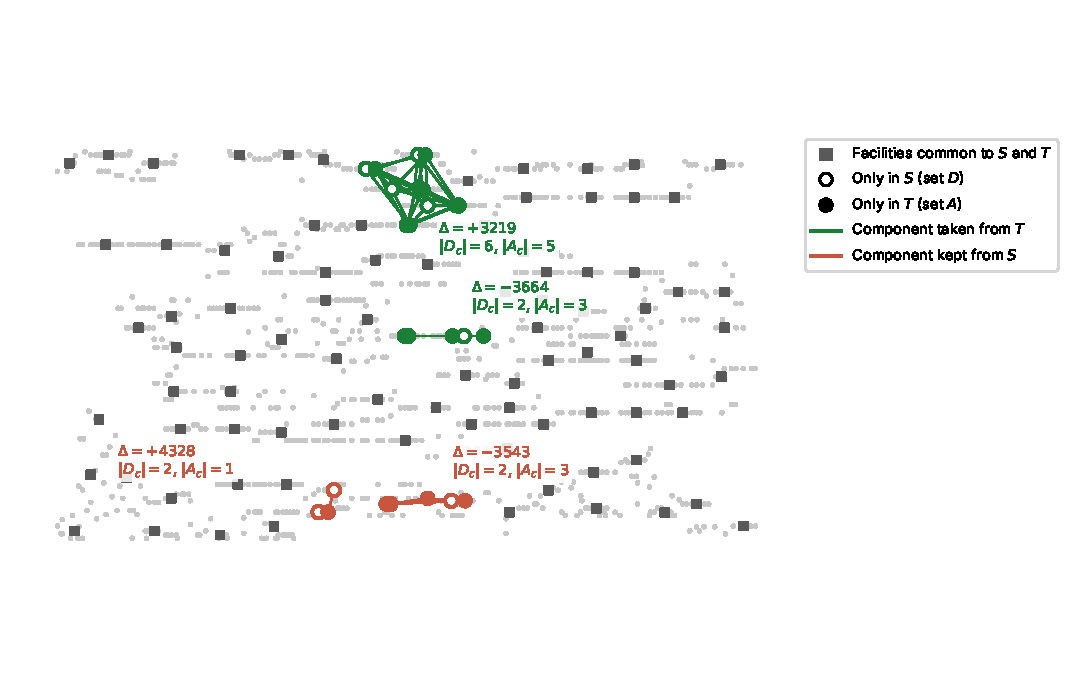
\includegraphics[width=0.95\linewidth]{images/fig_components.pdf}
  \caption{Components of two swap local optima of rl1304 with $p=100$: an incumbent $S$ with cost \mExZS{} and the solution $T$ obtained from it by a kick of 20 facilities followed by local search, with cost \mExZT. The \mExQ{} facilities in which they differ form \mExNC{} components. Each of the two components with a negative difference adds one facility, and each of the two others removes one. The balanced selection takes two components with a total difference of \mExGain, which gives a child with cost \mExZC, better than both parents, whereas an acceptance rule based on the total cost would discard $T$.}
  \label{fig:components}
\end{figure}

\subsection{Selecting the components}
Proposition~\ref{prop:bound} turns recombination into a selection problem: choose the set $K$ that minimizes $\sum_{c\in K}\Delta_c$ subject to $\sum_{c\in K}w_c=0$, where $w_c=|A_c|-|D_c|$ is the \emph{imbalance} of component $c$. A balanced component ($w_c=0$) is taken if and only if $\Delta_c<0$. The unbalanced components are coupled by the constraint, and the problem restricted to them is solved exactly by dynamic programming. Let the unbalanced components be numbered $1,\dots,c_u$ and let $F_j(b)$ be the minimum of $\sum_{c\in K}\Delta_c$ over the sets $K\subseteq\{1,\dots,j\}$ with $\sum_{c\in K}w_c=b$. Then $F_0(0)=0$, $F_0(b)=\infty$ for $b\neq 0$, and
\begin{equation}
F_j(b)=\min\bigl\{F_{j-1}(b),\ F_{j-1}(b-w_j)+\Delta_j\bigr\},
\end{equation}
and the optimal selection is recovered from $F_{c_u}(0)$. Only the values $|b|\leq B=\tfrac12\sum_c|w_c|$ are needed, because a selection with zero total imbalance never has a partial sum outside this range. The child returned by BPX is $Y(K^*)$ for the optimal set $K^*$, followed by the local search of Section~\ref{sec:ls}.

\begin{corollary}
\label{cor:child}
The child of BPX satisfies $f\bigl(Y(K^*)\bigr)\leq\min\{f(S),f(T)\}$, with strict inequality whenever the optimal value of the selection problem is lower than $\min\{0,f(T)-f(S)\}$.
\end{corollary}
\begin{proof}
The empty set and the set of all components are feasible selections, with values $0$ and $f(T)-f(S)$. The claim follows from Proposition~\ref{prop:bound}.
\end{proof}

Unbalanced components are not a marginal case. When a kicked solution is re-optimized, the local search often ends with one facility more in one region and one fewer in another, as in Figure~\ref{fig:components}. Such a transfer of a facility between two regions appears as a pair of components with imbalances $+1$ and $-1$, and the dynamic programme pairs each component that gains by receiving a facility with the component that loses least by giving one up, which need not be the one chosen by the local search.

\paragraph{Verification.} The proposition and the implementation of the selection were checked by exhaustive enumeration. For \mVerPairs{} pairs formed by a local optimum of an OR-Library or TSPLIB-based instance and the local optimum reached after a kick of up to 24 facilities, every subset of the components was enumerated, \mVerSubsets{} subsets in all, and the corresponding solution was evaluated from scratch. The bound held for every subset, the selection returned by the dynamic programme was the best balanced subset in every pair, and the child was strictly better than both parents in \mVerStrict{} pairs. In this sample the bound was attained by all \mVerBalanced{} balanced subsets, so it is tight in practice, although it need not be in general.

\paragraph{Complexity.} With the closest facility and its distance stored for every customer of both parents, the components are obtained with a union--find structure in $O\bigl((n+p)\,\alpha(p)\bigr)$ time, where $\alpha$ is the inverse Ackermann function, the differences in $O(n)$, and the selection in $O(c_uB)$, with $c_u\leq 2q$ and $B\leq q$. Since the local search already maintains the closest facilities, BPX adds no evaluation of the objective function. Its cost is negligible compared with one scan of the swap neighbourhood.

\paragraph{Relation to partition crossover.} As in partition crossover for pseudo-Boolean functions \citep{tinos_2015}, the facilities shared by the parents are fixed, the remaining ones are split into components and each component is inherited as a whole. There are three differences. First, the components are defined through the assignments of the two parents rather than through a fixed interaction graph of the problem, and the separable function is an upper bound on the cost and not the cost itself. Second, the offspring is the best with respect to this bound among the selections that satisfy the cardinality constraint, which requires an optimization over the unbalanced components. Third, the child is not necessarily a swap local optimum and is passed to the local search. BPX is deterministic and has no parameter.

% =====================================================================
\section{The \BPX{} algorithm}
\label{sec:method}

\subsection{Swap local search}
\label{sec:ls}
All algorithms of this study share one local search: the best-improvement swap local search, run until no improving swap exists. A solution is a set $S$ of $p$ sites, stored as a sorted vector. For every customer $i$ the search keeps the closest and second-closest open facilities, at distances $d^1_i$ and $d^2_i$. Following \citet{resende_werneck_2003_impl, resende_fast_2007}, the profit of closing $u\in S$ and opening $r\notin S$ is written as $\mathrm{gain}(r)-\mathrm{loss}(u)+\mathrm{extra}(u,r)$, where
\begin{align*}
\mathrm{gain}(r)&=\sum_{i}\max\bigl(0,\,d^1_i-C_{ir}\bigr), \qquad
\mathrm{loss}(u)=\sum_{i:\,\phi_i=u}\bigl(d^2_i-d^1_i\bigr),\\
\mathrm{extra}(u,r)&=\sum_{i:\,\phi_i=u,\ C_{ir}<d^2_i}\bigl(d^2_i-\max(C_{ir},d^1_i)\bigr),
\end{align*}
and $\phi_i$ is the closest open facility of $i$. Our implementation recomputes these quantities in every scan but visits, for each customer, only the sites that can contribute. The sites are stored for every customer in order of increasing distance; $\mathrm{gain}$ receives contributions from the sites closer than $d^1_i$ and $\mathrm{extra}$ from those closer than $d^2_i$, so the enumeration for customer $i$ stops at the first site at distance $d^2_i$ or more. The pairs $(u,r)$ that share no customer have $\mathrm{extra}(u,r)=0$, and the best of them is obtained from the largest gain and the smallest loss. A scan therefore costs $O\bigl(n+p+\sum_i|\{r: C_{ir}<d^2_i\}|\bigr)$ and evaluates the swap neighbourhood exactly. When $p$ is large the second-closest facility of a customer is near and the lists are short. Table~\ref{tab:speed} compares the time per scan with that of an implementation of the fast interchange of \citet{whitaker_1983}, which costs $O(mn)$ per scan, on \mSpCases{} instance--$p$ pairs, with complete local searches from the same three random solutions. The ratio ranges from \mSpMin{} to \mSpMax{} and is between \mSpBigMin{} and \mSpBigMax{} for $p\geq 50$; every local optimum returned was confirmed to be a local optimum by the other implementation. The sorted lists take $O(n^2)$ memory and are computed once per instance.

\begin{table}[htbp]
\centering
\caption{Time per neighbourhood scan of the fast interchange divided by that of the local search used in this study (complete local searches from the same three random solutions).}
\label{tab:speed}
\small
\begin{tabular}{lrrr@{\hskip 18pt}lrrr}
\toprule
Instance & $n$ & $p$ & Ratio & Instance & $n$ & $p$ & Ratio \\
\midrule
pmed5 & 100 & 33 & 2.8 & fl1400 & 1400 & 10 & 2.8 \\
pmed10 & 200 & 67 & 4.9 & fl1400 & 1400 & 50 & 6.1 \\
pmed15 & 300 & 100 & 7.3 & fl1400 & 1400 & 100 & 9.7 \\
pmed20 & 400 & 133 & 9.8 & fl1400 & 1400 & 300 & 30.6 \\
pmed25 & 500 & 167 & 13.5 & fl1400 & 1400 & 500 & 33.3 \\
pmed30 & 600 & 200 & 15.1 & d2103 & 2103 & 10 & 2.7 \\
pmed34 & 700 & 140 & 17.5 & d2103 & 2103 & 50 & 6.9 \\
pmed37 & 800 & 80 & 13.0 & d2103 & 2103 & 100 & 12.8 \\
pmed40 & 900 & 90 & 15.0 & d2103 & 2103 & 300 & 35.1 \\
pmed38 & 900 & 5 & 1.8 & d2103 & 2103 & 500 & 44.4 \\
pmed39 & 900 & 10 & 3.0 &  & & &  \\
\bottomrule
\end{tabular}
\end{table}

\subsection{Multi-kick search with BPX}
\label{sec:multikick}
\BPX{} (Algorithm~\ref{alg:mkbpx}) maintains an elite solution $S$, which is a swap local optimum, and a kick size $k$. In each iteration, $k$ randomly chosen facilities of $S$ are replaced by $k$ randomly chosen closed sites and the result is re-optimized by the local search, which gives an offspring $T$. If $T$ is better than $S$, the roles are exchanged, so that $T$ becomes the base and $S$ the donor. The base is then recombined with the donor by BPX. If the selection is not empty, the child is re-optimized and replaces the base when it is better. The best of the solutions obtained becomes the new elite solution. The kick size follows the schedule of basic VNS \citep{hansen_variable_1997}: it is reset to 1 after every improvement and increased by one otherwise, returning to 1 after $k_{\max}=p$. The search starts from a random solution improved by the local search and stops at a time limit.

In genetic terms, \BPX{} is a steady-state memetic algorithm with a population of one elite individual: the kick is the mutation, BPX the crossover between the offspring and its parent, and replacement is elitist. With the crossover removed, the algorithm is exactly basic VNS. This is the control used in the experiments, and it means that every difference observed between the two is due to BPX.

\begin{algorithm}[htbp]
\caption{\BPX: multi-kick search with balanced partition crossover}
\label{alg:mkbpx}
\begin{algorithmic}[1]
\Require Distance matrix $C$, number of medians $p$, time limit
\Ensure Best solution found
\State $S \gets \textsc{LocalSearch}(\text{random solution})$; \quad $k \gets 1$
\While{time limit not reached}
    \State $T \gets \textsc{LocalSearch}\bigl(\textsc{Kick}(S,k)\bigr)$ \Comment{replace $k$ random facilities by $k$ random closed sites}
    \If{$f(T) < f(S)$} $(B, R) \gets (T, S)$ \Else{} $(B, R) \gets (S, T)$ \EndIf \Comment{base and donor}
    \State $K^* \gets$ optimal balanced selection of the components of $(B,R)$ \Comment{Section~\ref{sec:bpx}}
    \If{$K^*\neq\emptyset$}
        \State $Y \gets \textsc{LocalSearch}\bigl(Y(K^*)\bigr)$
        \If{$f(Y) < f(B)$} $B \gets Y$ \EndIf
    \EndIf
    \If{$f(B) < f(S)$} $S \gets B$; $k \gets 1$
    \Else{} $k \gets k+1$; \textbf{if} $k>k_{\max}$ \textbf{then} $k\gets 1$
    \EndIf
\EndWhile
\State \Return $S$
\end{algorithmic}
\end{algorithm}

\subsection{Batch variant}
\label{sec:batch}
The algorithm extends naturally to several offspring per generation. In \BPXf, four copies of the elite solution are kicked and recombined with it as in Algorithm~\ref{alg:mkbpx}, each copy with its own kick-size counter. At the end of the round the best of the four results is recombined by BPX with each of the other three, and the outcome replaces all four copies. This variant corresponds to a population of four elite individuals that are fused in every generation, and it is used in Section~\ref{sec:res_factors} to examine whether a larger population pays.

% =====================================================================
\section{Experimental design}
\label{sec:design}

\subsection{Instances}
Two families of instances with known optimal or best-known values were used (Table~\ref{tab:instances}).
\begin{itemize}
    \item \emph{OR-Library.} The 40 instances pmed1--pmed40 \citep{beasley_1985, beasley_or_library_1990} are random graphs with $n=100$ to 900 vertices, shortest-path distances and $p=5$ to 200.
    \item \emph{TSPLIB.} Seven instances of the TSPLIB \citep{reinelt_1991} with 1304 to 5934 points were used with values of $p$ for which \citet{duran_mateluna_efficient_2023} report optimal or best-known values, and with their distance, the Euclidean distance rounded down to the nearest integer. Every customer location is a candidate site. This gives 57 instance--$p$ pairs. That study proves the optimality of most of these values; for a few pairs, among them fl1400 with $p=500$, u1432 with $p=400$ and d2103 with $p=50$, it reports the best value found within its time limit. The \emph{reference value} $f^*$ of a pair is the published value or, if one of our runs found a better solution, the best value found in our runs. \mRefSentence{} The distances were computed in double precision without any tolerance before rounding down; with this convention the published value was reached exactly by at least one of our runs in \mNRefReached{} of the \mNTspPairs{} pairs, which confirms that the instances coincide with those of the reference study.
\end{itemize}
The algorithm was developed on two of the TSPLIB instances, rl1304 and pcb3038 (19 pairs): the design decisions described in Section~\ref{sec:development} were taken with runs on six of these pairs. The other five TSPLIB instances (\mTPairs{} pairs) were not used in any way before the final campaign and form the \emph{test set}, on which the primary hypothesis is evaluated. Results on the development pairs are reported separately. The OR-Library instances had been used in the earlier study mentioned in Section~\ref{sec:intro}, but not to develop the crossover; they are reported as a second benchmark for comparison with the literature.

\begin{table}[htbp]
\centering
\caption{Instances, time limits and numbers of runs. Reference values for the TSPLIB-based pairs are the optimal or best-known values of \citet{duran_mateluna_efficient_2023}.}
\label{tab:instances}
\small
\resizebox{\textwidth}{!}{%
\begin{tabular}{llrlrr}
\toprule
Set & Instance & $n$ & Values of $p$ & Time limit (s) & Runs \\
\midrule
Test & fl1400 & 1400 & 5, 10, 20, 50, 100, 200, 300, 400, 500 & 10 & 10 \\
Test & u1432 & 1432 & 5, 10, 20, 50, 100, 200, 300, 400, 500 & 10 & 10 \\
Test & d2103 & 2103 & 5, 10, 20, 50, 100, 200, 300, 400, 500 & 20 & 10 \\
Test & fl3795 & 3795 & 50, 100, 150, 200, 300, 400, 500 & 40 & 5 \\
Test & rl5934 & 5934 & 200, 300, 400, 500 & 60 & 5 \\
Development & rl1304 & 1304 & 5, 10, 20, 50, 100, 200, 300, 400, 500 & 10 & 10 \\
Development & pcb3038 & 3038 & 5, 10, 20, 50, 100, 150, 200, 300, 400, 500 & 30 & 5 \\
\midrule
OR-Library & pmed1--pmed40 & 100--900 & 5--200 & 0.02--7.7 & 30 \\
\bottomrule
\end{tabular}}
\end{table}

\subsection{Algorithms compared}
\label{sec:algos}
Four algorithms were run with the same code, in which the crossover and the number of copies of the elite solution are options.
\begin{itemize}
    \item \emph{VNS}: basic VNS with $k_{\max}=p$, as in \citet{hansen_variable_1997}. It is Algorithm~\ref{alg:mkbpx} with the crossover removed, so that $T$ simply replaces $S$ when it is better, and it is the control for the effect of BPX.
    \item \emph{\BPX}: Algorithm~\ref{alg:mkbpx}, with the same schedule, $k_{\max}=p$.
    \item \emph{\VNSs}: VNS with a short shaking cycle, $k_{\max}=\min(p,20)$. During development this value gave VNS a lower mean gap than $k_{\max}=p$ (Section~\ref{sec:development}), so \VNSs{} serves as a tuned control.
    \item \emph{\BPXf}: the batch variant of Section~\ref{sec:batch}.
\end{itemize}
VNS and \BPX{} were run on all instances; \VNSs{} and \BPXf{} on the four TSPLIB instances with up to 2103 nodes. All algorithms start from a random solution and are stopped at the same time limit, which includes the initial local search. The limits (Table~\ref{tab:instances}) were fixed in advance and grow with the size of the instance; on the OR-Library instances they are the mean running times, instance by instance, of the earlier genetic algorithm, so that the results can be set beside those of that study.

\paragraph{State-of-the-art reference: PopStar.}
The four algorithms above answer the question of what the crossover adds to a perturbation-based search. To place \BPX{} with respect to the state of the art, it was also compared with the hybrid heuristic of \citet{resende_hybrid_2004}, a GRASP with path-relinking distributed as PopStar, which is the reference heuristic for the $p$MP on the classical benchmark sets and the usual source of upper bounds for exact methods \citep{garcia_2011}. Its published results cannot be set beside ours: they were obtained on another machine, with a stopping rule based on a number of iterations and with real-valued Euclidean distances, whereas the reference values used here are for distances rounded down. PopStar was therefore re-implemented from its description on the kernels of this study, so that the two algorithms differ in nothing but the search strategy: same language and compiler, same distance matrices and sorted lists, same random generator and clock, and the same swap local search (Section~\ref{sec:ls}), which evaluates the neighbourhood exactly as the local search of the original implementation does. The re-implementation follows the published algorithm component by component. (i)~\emph{Construction}: the sample greedy algorithm, which at each step evaluates $\lceil\log_2(m/p)\rceil$ randomly chosen sites and opens the most profitable one. (ii)~\emph{Multistart phase}: every constructed solution is improved by local search and combined by path-relinking with a solution of a pool of ten elite solutions, chosen with probability proportional to its difference from the new solution; the path goes from the better to the worse of the two by the most profitable swap at each step, and its best local minimum is improved by local search. (iii)~\emph{Pool}: a solution enters the pool only if it differs in at least four facilities from every better elite solution, and it replaces the most similar elite solution of equal or higher cost. (iv)~\emph{Post-optimization}: after 32 multistart iterations, every pair of elite solutions is relinked, from the worse to the better; the results form a new generation, and generations follow one another while they improve. The parameters are the published defaults (32 iterations, ten elite solutions). The path-relinking step was implemented with the gain, loss and extra quantities of the local search restricted to the facilities in which the two solutions differ, so that a step costs at most one neighbourhood scan, and it was verified against a brute-force implementation that evaluates every candidate swap from scratch (identical paths and identical results in \mPVerPairs{} pairs of local optima).

The only departure from the published algorithm is the stopping rule, which must be the time limit shared by all algorithms. When a cycle of 32 iterations and post-optimization ends before the limit, a new cycle starts with the elite pool retained, so that PopStar uses its whole budget and keeps what it has learnt; when the limit is reached the best solution found is returned. The number of iterations per cycle is the one parameter that this rule could interact with, and it was chosen on the development pairs, exactly as the design of \BPX{} was (Section~\ref{sec:development}). The fidelity of the re-implementation to the published results is examined in Section~\ref{sec:res_sota}.

\paragraph{The original PopStar program.}
A re-implementation isolates the search strategy, but it leaves open whether it does justice to the original. In a third campaign \BPX{} and VNS were therefore compared with the program of \citet{resende_hybrid_2004} itself, POPSTAR (version 20041104), as distributed by its authors.\footnote{\url{https://mauricio.resende.info/popstar/downloads.html}. The pre-compiled Linux executable offered there is a 32-bit binary built in 2002 that the dynamic loader of current systems no longer starts, so the source code of the same distribution was compiled, without any modification, with g++~13.3 and the option \texttt{-O3}.} The program is written in C++ and has its own local search, the swap procedure with incremental updates of \citet{resende_fast_2007}. It reads a full distance matrix, and it was given exactly the matrices used by the other algorithms (shortest-path distances for the OR-Library instances, Euclidean distances rounded down for the TSPLIB-based ones), so that all programs minimize the same objective function; every solution it wrote was re-evaluated with our code and gave the value that the program reported. POPSTAR stops after a number of iterations and has no time limit. Since it was not modified, the comparison was made at equal elapsed time (Section~\ref{sec:implementation}), in two configurations that were fixed before the runs. In what follows PopStar denotes the heuristic and its re-implementation, and POPSTAR the program of its authors.
\begin{itemize}
  \item \emph{Published configuration}: 32 multistart iterations and ten elite solutions, the setting of all the results of \citet{resende_hybrid_2004}. The program takes whatever time it needs, and the other algorithms are evaluated at that time.
  \item \emph{Scaled to the time limit}: ten elite solutions and a number of multistart iterations chosen, pair by pair, so that a run takes about 90\% of the time limit of Table~\ref{tab:instances}. Increasing the number of iterations is the way to trade time for quality indicated by the authors of the program. The number is computed from the runs of the published configuration of the same pair, made minutes earlier: if $a$ is the mean elapsed time of one multistart iteration, $b$ that of the post-optimization, $o$ that of the initialization and $T$ the time limit, then $k=\lfloor(0.9\,T-o-b)/a\rfloor$. Pairs with $k\geq 40$ are run with $k$ iterations; in the others the published configuration already uses the time limit, and its runs stand for this configuration as well.
\end{itemize}
No parameter of POPSTAR other than the number of iterations was changed, and neither \BPX{} nor VNS was modified or tuned for this campaign.

\subsection{Implementation and measurements}
\label{sec:implementation}
The algorithms were implemented in Python~3.13 with NumPy~2.5 and compiled with Numba~0.68. Every run is single-threaded and draws all its random numbers from one generator, seeded with a value determined by the algorithm, the instance, $p$ and the run index. The sequence of solutions visited by a run is therefore reproducible exactly, whereas the point at which the time limit stops it depends on the machine. Experiments were run on a Linux virtual machine with two Intel Xeon cores at 2.1~GHz, one run per core at a time. Times are elapsed times of the single-threaded process; reading the instance, computing the distance matrix and the sorted site lists, and the just-in-time compilation are excluded, as they are common to all algorithms. For every run we stored the seed, the best value, the numbers of iterations, of improvements accepted directly and through the crossover, of crossover calls, of components found and taken, of neighbourhood scans, the time of the first visit to the published value and the time and value of every improvement. Every returned solution was re-evaluated from scratch and checked for feasibility, and the bound of Proposition~\ref{prop:bound} was checked for every child.

\paragraph{Second campaign.} The comparison with PopStar was carried out in a second campaign on a virtual machine of the same type (two Intel Xeon cores at 2.1~GHz, same versions of Python, NumPy and Numba). Since a time limit makes results depend on the speed of the machine, the runs of the main campaign were not reused. Instead, PopStar and \BPX{} were run side by side, one process per core, on the same pairs in the same order, with the same time limits and numbers of runs as in Table~\ref{tab:instances}, so that the two algorithms were measured on the same hardware, at the same moment and under the same load. \BPX{} used the seeds of the main campaign: its runs visit the same sequences of solutions and differ from the earlier ones only in the point at which the limit stops them, which also gives a replication of the main results (Section~\ref{sec:res_sota}). An algorithm checks the clock between operations, so an operation that starts before the limit ends after it. To give neither algorithm an advantage from this overrun, in the second campaign the value of a run is the best value found \emph{within} the time limit, read from the stored trace of improvements, for both algorithms.

\paragraph{Third campaign.} The comparison with the original POPSTAR program was run on a virtual machine of the same type as those of the first two campaigns: Linux, two Intel Xeon cores at 2.1~GHz (CPU family~6, model~207) and 8~GB of memory, with the same versions of Python, NumPy and Numba. Virtual machines of one type need not be the same physical host, so, as in the second campaign, no log of an earlier campaign was reused: \BPX{} and VNS were run again, with the seeds of the main campaign, next to POPSTAR. The protocol has five elements.

\emph{Blocks.} The speed of a shared virtual machine is not constant. In a first attempt at this campaign, in which the programs were run one after the other over several hours, identical computations were 10 to 20\% faster after a restart of the virtual machine than before it, which is of the order of the differences that a comparison at equal time has to resolve. That attempt was discarded, and the campaign was blocked by instance--$p$ pair: all the runs of a pair, those of POPSTAR in its two configurations, those of \BPX{} and, on the test instances, those of VNS, were made within one block of \mXBlockMin{} to \mXBlockMax{} minutes (\mXBlockMean{} on average), always with two processes running, each pinned to one core, and with the runs of every algorithm alternating between the two cores. A slow drift of the machine therefore affects all the algorithms of a pair alike. As a check, the initialization of the distance oracle of POPSTAR, which is the same computation in its two configurations, differed by \mXOracleIn\% on average between the two sets of runs of a block.

\emph{Clocks.} The time of a run of VNS or \BPX{} is the elapsed time from the start of the search, as before, plus the time needed to sort the site lists (\mXOrderMin{} to \mXOrderMax~s, depending on the instance, measured on this machine), because the time of POPSTAR includes the initialization of its distance oracle; reading the instance is excluded for all programs. POPSTAR reports the user CPU time of its search, which cannot be set beside an elapsed time. Its elapsed time was therefore measured from outside, without touching the program, by time-stamping the progress lines that it writes while it runs; this also gives the time and value of every improvement of its best solution. On the TSPLIB-based pairs the elapsed time exceeded the reported CPU time by \mXClockPop\% on average. POPSTAR allocates and frees its auxiliary matrices in every local search; with the default settings of the C library this memory is returned to the operating system and mapped again each time, which on the instances with more than 3000 nodes cost about as much kernel time as the search itself. The allocator was therefore configured, through its environment variables, to keep freed memory in the process. This changes nothing in the algorithm and can only favour POPSTAR.

\emph{Equal-time rule.} For each instance--$p$ pair and each configuration of POPSTAR, let $t$ be the mean elapsed time of the POPSTAR runs of the pair. The value of a run of \BPX{} or VNS is the best value that the run had found at time $t$, read from its trace of improvements. To make this possible the runs were not stopped at the time limit $T$ of Table~\ref{tab:instances} when POPSTAR needed more: they continued, on the same trajectory, until 1.1 times the longest POPSTAR run of the block. The values at $T$ were recorded as well.

\emph{Disturbances.} Every run was checked: a run of VNS or \BPX{} whose CPU time fell below 98.5\% of its elapsed time, or a run of POPSTAR whose elapsed time exceeded its CPU time by more than 5\% plus 0.15~s, was discarded and repeated, at most twice. This happened in \mXRepeatBpx{} of the \mXNRunsOurs{} runs of VNS and \BPX{} (\mXRepeatBpxTsp{} on the TSPLIB-based pairs; the others on OR-Library instances, whose runs last a fraction of a second) and in \mXRepeatPop{} of the \mXNRunsPop{} runs of POPSTAR, most of them runs of the scaled configuration in which the kernel time of the program itself, \mXSysPop\% of its CPU time on average, came close to the threshold.

\emph{Exact replay and complete traces.} A run of VNS or \BPX{} is determined by its seed, and the main campaign logged the seed and the number of iterations of every run. The main campaign had not stored the improvement traces of VNS and \BPX{} on fl1400, u1432 and rl1304. To complete them, the \mXReplayRuns{} runs of the two algorithms on the four instances with up to 2103 nodes were repeated with their seeds for at least the logged number of iterations, and the value after that number of iterations was compared with the logged value: the two coincided in all \mXReplayOk{} runs. The main campaign can thus be reproduced exactly on another machine. The replay supplied the \mXTraceAdded{} missing traces (their values are exact, and their times are rescaled to the clock of the original run) and confirmed, value by value, the \mXTraceChecked{} traces of these runs that had been stored. The improvement traces of all runs of all campaigns are part of the supplementary material.

\subsection{Performance measures and statistical methodology}
For each instance--$p$ pair and algorithm we report the mean gap $100(\bar f-f^*)/f^*$ over the runs and the number of runs that reached the reference value (hits); for brevity such runs are called optimal, although for a few pairs the reference value is not proven optimal. Aggregates are the average of the mean gaps over the pairs, the share of optimal runs and the number of pairs in which every run was optimal. Following \citet{demsar_2006} and \citet{derrac_2011}, the pair is the unit of analysis. Two algorithms are compared with the two-sided Wilcoxon signed-rank test \citep{wilcoxon_1945} on the mean gaps, with zero differences discarded and the exact distribution of the statistic (no ties occurred among the non-zero differences), together with the numbers of pairs won, lost and tied and the mean difference in percentage points (p.p.) with a percentile bootstrap 95\% confidence interval from $2\times10^4$ resamples of the pairs \citep{efron_tibshirani_1993}. Four hypotheses are declared, and their $P$-values are adjusted with Holm's procedure \citep{holm_1979}: H1, \BPX{} versus VNS on the test set (the primary hypothesis); H2, \BPX{} versus VNS on the OR-Library instances; H3, \BPX{} versus \VNSs{} on the test pairs on which both were run; H4, \BPXf{} versus \BPX{} on the same pairs. The second campaign has its own family of two hypotheses, declared before it was run and adjusted in the same way: H5, PopStar versus \BPX{} on the test set; H6, PopStar versus \BPX{} on the OR-Library instances. The third campaign has a family of two hypotheses as well, also declared before it was run: H7, the original POPSTAR program in its published configuration versus \BPX{} at equal elapsed time on the test set; H8, the same comparison with POPSTAR scaled to the time limit. Other statistics are descriptive. To avoid confusion with the number of medians, $P$ denotes $P$-values.

\subsection{Development}
\label{sec:development}
Design decisions were taken on six development pairs (rl1304 with $p=100$, 300 and 500 and a 10~s limit; pcb3038 with the same values and a 40~s limit), with two runs per configuration. Table~\ref{tab:dev} lists the configurations that were evaluated on these pairs; two further variants with two and four elite solutions that were fused only every five rounds and otherwise kept distinct had mean gaps of 0.020\% and 0.018\%. Three observations determined the final design. First, adding BPX to VNS reduced the mean gap fivefold. Second, the shaking range matters in opposite ways: VNS is better with a short cycle, whereas \BPX{} is better with the full cycle, which is consistent with the purpose of the crossover, since large kicks perturb many regions at once and only a recombination can keep the successful ones. Third, neither accepting components with zero difference (to move across plateaus) nor evolving several elite solutions that are fused periodically improved on the single-elite algorithm. The simplest configuration, which has no parameter beyond those of basic VNS, was therefore retained, and the batch variant with four copies was kept as a factor of the final study. Earlier exploratory prototypes without the crossover, in which elite solutions were recombined by exchanging random subsets of their exclusive facilities, were not better than VNS and were abandoned.

The time-limited PopStar was configured on the same six pairs with the same protocol (Table~\ref{tab:devpop}). Cycles of 32 multistart iterations, the published default, gave the lowest mean gap (\mPDevA\%, against \mPDevB\% for 16 iterations and \mPDevC\% for 8), so the default configuration was retained. With shorter cycles the post-optimization runs more often but on pools that are less diverse.

\begin{table}[htbp]
\centering
\caption{Configurations tried during development: mean gap (\%) over two runs on the six development pairs. The last two rows are variants with two and four elite solutions fused after every round.}
\label{tab:dev}
\small
\resizebox{\textwidth}{!}{%
\begin{tabular}{lrrrrrrr}
\toprule
 & \multicolumn{3}{c}{rl1304 (10 s)} & \multicolumn{3}{c}{pcb3038 (40 s)} & \\
\cmidrule(lr){2-4}\cmidrule(lr){5-7}
Configuration & $p=100$ & 300 & 500 & $p=100$ & 300 & 500 & Mean \\
\midrule
VNS, $k_{\max}=p$ & 0.0135 & 0.0116 & 0.0495 & 0.0679 & 0.1218 & 0.0757 & 0.0566 \\
VNS, $k_{\max}=20$ & 0.0136 & 0.0073 & 0.0155 & 0.0293 & 0.0629 & 0.0864 & 0.0358 \\
\BPX, $k_{\max}=p$ (retained) & 0.0000 & 0.0000 & 0.0000 & 0.0185 & 0.0102 & 0.0356 & 0.0107 \\
\BPX, $k_{\max}=0.2p$ & 0.0273 & 0.0023 & 0.0000 & 0.0293 & 0.0112 & 0.0356 & 0.0176 \\
\BPX, $k_{\max}=20$ & 0.0273 & 0.0037 & 0.0155 & 0.0293 & 0.0664 & 0.0898 & 0.0386 \\
\BPX, zero-difference components accepted & 0.0000 & 0.0000 & 0.0000 & 0.0482 & 0.0206 & 0.0430 & 0.0186 \\
\BPX, two elite solutions & 0.0000 & 0.0000 & 0.0000 & 0.0075 & 0.0257 & 0.0427 & 0.0126 \\
\BPX, four elite solutions & 0.0000 & 0.0023 & 0.0000 & 0.0172 & 0.0254 & 0.0382 & 0.0138 \\
\bottomrule
\end{tabular}}
\end{table}

\begin{table}[htbp]
\centering
\caption{Configuration of the time-limited PopStar: mean gap (\%) to the published value over two runs on the six development pairs, by number of multistart iterations per cycle (ten elite solutions).}
\label{tab:devpop}
\small
\begin{tabular}{lrrrrrrr}
\toprule
 & \multicolumn{3}{c}{rl1304 (10 s)} & \multicolumn{3}{c}{pcb3038 (40 s)} & \\
\cmidrule(lr){2-4}\cmidrule(lr){5-7}
Iterations per cycle & $p=100$ & 300 & 500 & $p=100$ & 300 & 500 & Mean \\
\midrule
32 (default, retained) & 0.0159 & 0.0042 & 0.0144 & 0.0115 & 0.0265 & 0.0423 & 0.0191 \\
16 & 0.0000 & 0.0056 & 0.0155 & 0.0104 & 0.0490 & 0.0556 & 0.0227 \\
8 & 0.0000 & 0.0023 & 0.0072 & 0.0156 & 0.0624 & 0.0619 & 0.0249 \\
\bottomrule
\end{tabular}
\end{table}

% =====================================================================
\section{Results}
\label{sec:results}

\subsection{Effect of the crossover on the test set}
\label{sec:res_main}
Tables~\ref{tab:pairs1} and~\ref{tab:pairs2} give the results for every TSPLIB-based pair, Table~\ref{tab:summary} aggregates them and Figure~\ref{fig:pairs} shows the mean gaps of VNS and \BPX{} side by side. On the \mTPairs{} test pairs, none of which was used during development, the mean gap fell from \mTvnsGap\% with VNS to \mTbpxGap\% with \BPX, a ratio of \mTRatio, and the share of the \mTRuns{} runs that ended at the reference value rose from \mTvnsHit\% to \mTbpxHit\%. \BPX{} had the lower mean gap in \mTW{} pairs, VNS in \mTL{} (\mTLostList), and they tied in \mTT, all of them pairs in which every run of both algorithms was optimal. The mean difference was \mTDiff~p.p.\ (95\% CI \mTLo--\mTHi) and the primary hypothesis H1 is rejected ($P=\mHoneP$; Holm-adjusted $P=\mHonePadj$; Table~\ref{tab:tests}). The largest mean gap of a pair was \mTbpxMax\% for \BPX{} and \mTvnsMax\% for VNS.

The difference is concentrated where the problem is hard. With $p\leq 20$ the two algorithms are indistinguishable (Table~\ref{tab:mech}), because nearly all their runs reach the reference value. On the \mTbigPairs{} test pairs with $p\geq100$, the mean gap is \mTbigvnsGap\% for VNS and \mTbigbpxGap\% for \BPX, and the shares of optimal runs are \mTbigvnsHit\% and \mTbigbpxHit\%. These shares are low for both algorithms because the time limits are short for instances of this size; Section~\ref{sec:res_long} examines longer runs. On the two largest instances, fl3795 and rl5934, whose time limits allow only a few hundred iterations, the mean gaps are \mFlvnsGap\% against \mFlbpxGap\% and \mRlvnsGap\% against \mRlbpxGap\%. The development pairs, reported for completeness, show the same pattern (mean gap \mDvnsGap\% against \mDbpxGap\%; \BPX{} better in \mDW{} of \mDPairs{} pairs and worse in \mDL). Figure~\ref{fig:anytime} shows the mean gap as a function of time on four test pairs. The curves of the two algorithms coincide during the initial descent, in which the crossover finds nothing to select, and separate afterwards: VNS goes through long periods without improvement, whereas \BPX{} keeps improving.

\begin{table}[htbp]
\centering
\caption{Aggregate results. Mean gap: average over the pairs of the mean gap of the runs. Optimal runs: share of runs that ended at the reference value. All runs optimal: number of pairs in which every run did. Within each block all algorithms are compared on the same pairs.}
\label{tab:summary}
\small
\setlength{\tabcolsep}{4pt}
\resizebox{\textwidth}{!}{\begin{tabular}{llrrrrrr}
\toprule
Set & Algorithm & Pairs & Runs & Mean gap (\%) & Max mean gap (\%) & Optimal runs (\%) & All runs optimal \\
\midrule
Test set & VNS & 38 & 325 & 0.1632 & 0.7168 & 34.8 & 11/38 \\
 & MK-BPX & 38 & 325 & 0.0679 & 0.4797 & 44.9 & 11/38 \\
\midrule
Test set, $n\leq 2103$ & VNS & 27 & 270 & 0.1519 & 0.7168 & 40.7 & 11/27 \\
 & VNS$_{20}$ & 27 & 270 & 0.1161 & 0.6573 & 43.3 & 11/27 \\
 & MK-BPX & 27 & 270 & 0.0480 & 0.4409 & 52.2 & 11/27 \\
 & MK-BPX$_{4}$ & 27 & 270 & 0.0445 & 0.4553 & 51.1 & 11/27 \\
\midrule
Development pairs & VNS & 19 & 140 & 0.0366 & 0.1119 & 47.9 & 7/19 \\
 & MK-BPX & 19 & 140 & 0.0128 & 0.0659 & 76.4 & 11/19 \\
\midrule
OR-Library & VNS & 40 & 1200 & 0.0003 & 0.0059 & 99.1 & 37/40 \\
 & MK-BPX & 40 & 1200 & 0.0000 & 0.0000 & 100.0 & 40/40 \\
\bottomrule
\end{tabular}}
\end{table}

\begin{figure}[htbp]
  \centering
  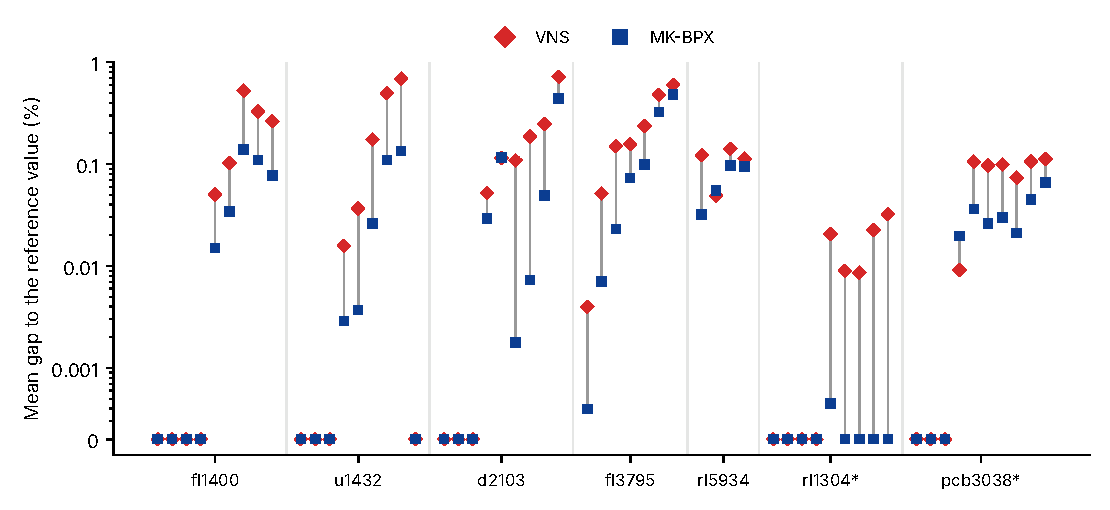
\includegraphics[width=\linewidth]{images/fig_pairs.pdf}
  \caption{Mean gap to the reference value of VNS and \BPX{} on the 57 TSPLIB-based pairs, grouped by instance and ordered by increasing $p$ within each instance (logarithmic scale; the bottom line corresponds to a mean gap of zero). An asterisk marks the two development instances.}
  \label{fig:pairs}
\end{figure}

\begin{table}[htbp]
\centering
\caption{Paired comparisons of mean gaps. The difference is $x-y$, so a positive value favours $y$. CI: percentile bootstrap over pairs. $P$: two-sided Wilcoxon signed-rank test with zero differences discarded; H1--H4 are adjusted with Holm's procedure, and the rows below the rule are descriptive.}
\label{tab:tests}
\footnotesize
\setlength{\tabcolsep}{3pt}
\resizebox{\textwidth}{!}{\begin{tabular}{llrrrrrr}
\toprule
Hypothesis & $x$ vs.\ $y$ & Pairs & $y$ better / worse / tie & Mean diff.\ (p.p.) & 95\% CI & $P$ & Holm $P$ \\
\midrule
H1: Crossover, test set & VNS vs.\ MK-BPX & 38 & 25 / 2 / 11 & +0.0953 & [+0.0573, +0.1387] & $1.0\times10^{-7}$ & $4.2\times10^{-7}$ \\
H2: Crossover, OR-Library & VNS vs.\ MK-BPX & 40 & 3 / 0 / 37 & +0.0003 & [+0.0000, +0.0007] & $0.250$ & $0.500$ \\
H3: Tuned control & VNS$_{20}$ vs.\ MK-BPX & 27 & 16 / 0 / 11 & +0.0682 & [+0.0337, +0.1087] & $3.1\times10^{-5}$ & $9.2\times10^{-5}$ \\
H4: Four elite copies & MK-BPX vs.\ MK-BPX$_{4}$ & 27 & 9 / 6 / 12 & +0.0035 & [-0.0009, +0.0084] & $0.277$ & $0.500$ \\
\midrule
Crossover, development pairs & VNS vs.\ MK-BPX & 19 & 11 / 1 / 7 & +0.0237 & [+0.0117, +0.0368] & $0.0024$ & -- \\
Shaking range of VNS & VNS vs.\ VNS$_{20}$ & 27 & 13 / 3 / 11 & +0.0357 & [+0.0161, +0.0574] & $0.0027$ & -- \\
\bottomrule
\end{tabular}}
\end{table}

\begin{figure}[htbp]
  \centering
  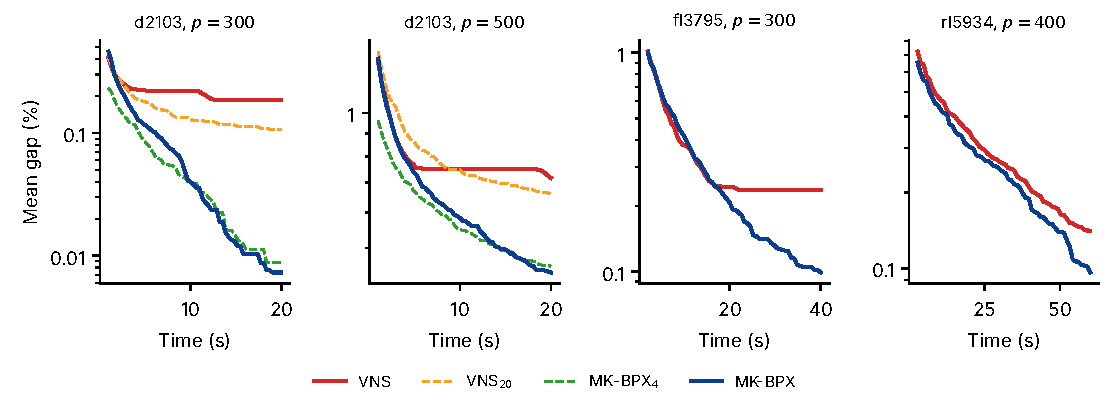
\includegraphics[width=\linewidth]{images/fig_anytime.pdf}
  \caption{Mean gap over the runs as a function of time on four test pairs, computed from the stored improvement traces.}
  \label{fig:anytime}
\end{figure}

\begin{table}[p]
\centering
\caption{Results on the TSPLIB-based instances with up to 2103 nodes (10 runs; time limit 10~s, and 20~s for d2103). Gap: mean gap to the reference value $f^*$ in \%. Hits: runs that reached $f^*$. The lowest mean gap of each row is in bold when the algorithms differ. $^{d}$: development instance.}
\label{tab:pairs1}
\footnotesize
\setlength{\tabcolsep}{3.5pt}
\renewcommand{\arraystretch}{0.88}
\resizebox{\textwidth}{!}{\begin{tabular}{lrrrrrrrrrr}
\toprule
Instance & $p$ & $f^*$ & \multicolumn{2}{c}{VNS} & \multicolumn{2}{c}{VNS$_{20}$} & \multicolumn{2}{c}{MK-BPX} & \multicolumn{2}{c}{MK-BPX$_{4}$} \\
\cmidrule(lr){4-5}\cmidrule(lr){6-7}\cmidrule(lr){8-9}\cmidrule(lr){10-11}
 & &  & Gap & Hits & Gap & Hits & Gap & Hits & Gap & Hits \\
\midrule
fl1400 & 5 & 174877 & 0.0000 & 10/10 & 0.0000 & 10/10 & 0.0000 & 10/10 & 0.0000 & 10/10 \\
fl1400 & 10 & 100601 & 0.0000 & 10/10 & 0.0000 & 10/10 & 0.0000 & 10/10 & 0.0000 & 10/10 \\
fl1400 & 20 & 57191 & 0.0000 & 10/10 & 0.0000 & 10/10 & 0.0000 & 10/10 & 0.0000 & 10/10 \\
fl1400 & 50 & 28486 & 0.0000 & 10/10 & 0.0000 & 10/10 & 0.0000 & 10/10 & 0.0000 & 10/10 \\
fl1400 & 100 & 15962 & 0.0501 & 0/10 & 0.0827 & 0/10 & \textbf{0.0150} & 7/10 & \textbf{0.0150} & 7/10 \\
fl1400 & 200 & 8806 & 0.1022 & 0/10 & 0.0897 & 0/10 & \textbf{0.0341} & 1/10 & 0.0386 & 0/10 \\
fl1400 & 300 & 6109 & 0.5238 & 0/10 & 0.3536 & 0/10 & 0.1391 & 0/10 & \textbf{0.1162} & 0/10 \\
fl1400 & 400 & 4648 & 0.3292 & 0/10 & 0.2582 & 0/10 & 0.1097 & 0/10 & \textbf{0.1054} & 0/10 \\
fl1400 & 500 & 3764 & 0.2630 & 0/10 & 0.1674 & 0/10 & 0.0770 & 0/10 & \textbf{0.0611} & 0/10 \\
\addlinespace[2pt]
u1432 & 5 & 1210126 & 0.0000 & 10/10 & 0.0000 & 10/10 & 0.0000 & 10/10 & 0.0000 & 10/10 \\
u1432 & 10 & 849759 & 0.0000 & 10/10 & 0.0000 & 10/10 & 0.0000 & 10/10 & 0.0000 & 10/10 \\
u1432 & 20 & 588766 & 0.0000 & 10/10 & 0.0000 & 10/10 & 0.0000 & 10/10 & 0.0000 & 10/10 \\
u1432 & 50 & 362072 & 0.0158 & 0/10 & 0.0068 & 3/10 & \textbf{0.0029} & 5/10 & 0.0067 & 3/10 \\
u1432 & 100 & 243793 & 0.0367 & 0/10 & 0.0090 & 3/10 & 0.0037 & 5/10 & \textbf{0.0032} & 5/10 \\
u1432 & 200 & 159887 & 0.1736 & 0/10 & 0.0841 & 0/10 & 0.0260 & 0/10 & \textbf{0.0214} & 0/10 \\
u1432 & 300 & 123689 & 0.4966 & 0/10 & 0.3736 & 0/10 & 0.1094 & 0/10 & \textbf{0.0924} & 0/10 \\
u1432 & 400 & 103979 & 0.6861 & 0/10 & 0.5323 & 0/10 & 0.1341 & 0/10 & \textbf{0.1104} & 0/10 \\
u1432 & 500 & 93200 & 0.0000 & 10/10 & 0.0000 & 10/10 & 0.0000 & 10/10 & 0.0000 & 10/10 \\
\addlinespace[2pt]
d2103 & 5 & 1005136 & 0.0000 & 10/10 & 0.0000 & 10/10 & 0.0000 & 10/10 & 0.0000 & 10/10 \\
d2103 & 10 & 687321 & 0.0000 & 10/10 & 0.0000 & 10/10 & 0.0000 & 10/10 & 0.0000 & 10/10 \\
d2103 & 20 & 482926 & 0.0000 & 10/10 & 0.0000 & 10/10 & 0.0000 & 10/10 & 0.0000 & 10/10 \\
d2103 & 50 & 302190 & 0.0521 & 0/10 & 0.0912 & 1/10 & \textbf{0.0294} & 0/10 & 0.0476 & 3/10 \\
d2103 & 100 & 194664 & 0.1144 & 0/10 & 0.1264 & 0/10 & 0.1166 & 0/10 & \textbf{0.0688} & 0/10 \\
d2103 & 200 & 117753 & 0.1084 & 0/10 & 0.0352 & 0/10 & \textbf{0.0018} & 7/10 & 0.0035 & 3/10 \\
d2103 & 300 & 90471 & 0.1854 & 0/10 & 0.1070 & 0/10 & \textbf{0.0073} & 6/10 & 0.0088 & 7/10 \\
d2103 & 400 & 75324 & 0.2468 & 0/10 & 0.1614 & 0/10 & 0.0489 & 0/10 & \textbf{0.0478} & 0/10 \\
d2103 & 500 & 64006 & 0.7168 & 0/10 & 0.6573 & 0/10 & \textbf{0.4409} & 0/10 & 0.4553 & 0/10 \\
\addlinespace[2pt]
rl1304$^{d}$ & 5 & 3099073 & 0.0000 & 10/10 & 0.0000 & 10/10 & 0.0000 & 10/10 & 0.0000 & 10/10 \\
rl1304$^{d}$ & 10 & 2134295 & 0.0000 & 10/10 & 0.0000 & 10/10 & 0.0000 & 10/10 & 0.0000 & 10/10 \\
rl1304$^{d}$ & 20 & 1412108 & 0.0000 & 10/10 & 0.0000 & 10/10 & 0.0000 & 10/10 & 0.0000 & 10/10 \\
rl1304$^{d}$ & 50 & 795012 & 0.0000 & 10/10 & 0.0000 & 10/10 & 0.0000 & 10/10 & 0.0000 & 10/10 \\
rl1304$^{d}$ & 100 & 491639 & 0.0206 & 2/10 & 0.0027 & 9/10 & 0.0004 & 9/10 & \textbf{0.0000} & 10/10 \\
rl1304$^{d}$ & 200 & 268573 & 0.0090 & 3/10 & \textbf{0.0000} & 10/10 & \textbf{0.0000} & 10/10 & \textbf{0.0000} & 10/10 \\
rl1304$^{d}$ & 300 & 177326 & 0.0086 & 1/10 & 0.0052 & 1/10 & \textbf{0.0000} & 10/10 & \textbf{0.0000} & 10/10 \\
rl1304$^{d}$ & 400 & 128332 & 0.0226 & 1/10 & 0.0002 & 9/10 & \textbf{0.0000} & 10/10 & \textbf{0.0000} & 10/10 \\
rl1304$^{d}$ & 500 & 97024 & 0.0323 & 2/10 & 0.0052 & 7/10 & \textbf{0.0000} & 10/10 & \textbf{0.0000} & 10/10 \\
\bottomrule
\end{tabular}}
\end{table}

\begin{table}[htbp]
\centering
\caption{Results on the TSPLIB-based instances with more than 3000 nodes (5 runs; time limits of 40~s for fl3795, 60~s for rl5934 and 30~s for pcb3038). Columns as in Table~\ref{tab:pairs1}.}
\label{tab:pairs2}
\footnotesize
\setlength{\tabcolsep}{4pt}
\renewcommand{\arraystretch}{0.9}
\begin{tabular}{lrrrrrr}
\toprule
Instance & $p$ & $f^*$ & \multicolumn{2}{c}{VNS} & \multicolumn{2}{c}{MK-BPX} \\
\cmidrule(lr){4-5}\cmidrule(lr){6-7}
 & &  & Gap & Hits & Gap & Hits \\
\midrule
fl3795 & 50 & 150940 & 0.0040 & 3/5 & \textbf{0.0004} & 4/5 \\
fl3795 & 100 & 88299 & 0.0514 & 0/5 & \textbf{0.0070} & 1/5 \\
fl3795 & 150 & 65868 & 0.1497 & 0/5 & \textbf{0.0231} & 0/5 \\
fl3795 & 200 & 53928 & 0.1569 & 0/5 & \textbf{0.0731} & 0/5 \\
fl3795 & 300 & 39586 & 0.2364 & 0/5 & \textbf{0.0990} & 0/5 \\
fl3795 & 400 & 31354 & 0.4778 & 0/5 & \textbf{0.3228} & 0/5 \\
fl3795 & 500 & 25976 & 0.5982 & 0/5 & \textbf{0.4797} & 0/5 \\
\addlinespace[2pt]
rl5934 & 200 & 1805530 & 0.1224 & 0/5 & \textbf{0.0321} & 0/5 \\
rl5934 & 300 & 1392419 & \textbf{0.0488} & 0/5 & 0.0553 & 0/5 \\
rl5934 & 400 & 1143940 & 0.1411 & 0/5 & \textbf{0.0963} & 0/5 \\
rl5934 & 500 & 972799 & 0.1127 & 0/5 & \textbf{0.0944} & 0/5 \\
\addlinespace[2pt]
pcb3038$^{d}$ & 5 & 1777835 & 0.0000 & 5/5 & 0.0000 & 5/5 \\
pcb3038$^{d}$ & 10 & 1211704 & 0.0000 & 5/5 & 0.0000 & 5/5 \\
pcb3038$^{d}$ & 20 & 839494 & 0.0000 & 5/5 & 0.0000 & 5/5 \\
pcb3038$^{d}$ & 50 & 506339 & \textbf{0.0092} & 3/5 & 0.0196 & 2/5 \\
pcb3038$^{d}$ & 100 & 351500 & 0.1053 & 0/5 & \textbf{0.0361} & 1/5 \\
pcb3038$^{d}$ & 150 & 280128 & 0.0968 & 0/5 & \textbf{0.0261} & 0/5 \\
pcb3038$^{d}$ & 200 & 237399 & 0.0992 & 0/5 & \textbf{0.0298} & 0/5 \\
pcb3038$^{d}$ & 300 & 186833 & 0.0734 & 0/5 & \textbf{0.0211} & 0/5 \\
pcb3038$^{d}$ & 400 & 156276 & 0.1062 & 0/5 & \textbf{0.0449} & 0/5 \\
pcb3038$^{d}$ & 500 & 134798 & 0.1119 & 0/5 & \textbf{0.0659} & 0/5 \\
\bottomrule
\end{tabular}
\end{table}

\subsection{How the crossover works}
\label{sec:res_mech}
Table~\ref{tab:mech} relates the behaviour of BPX to the number of medians. Four facts stand out. First, the crossover costs nothing measurable. \BPX{} performs on average \mIterRatio{} times as many iterations as VNS in the same time, that is, more and not fewer: improvements are more frequent, every improvement resets the kick size to one, and small kicks are cheaper to repair than large ones. Second, in the great majority of calls no component can be taken, because the offspring is worse than the incumbent in every region or because the improving components cannot be balanced; a non-empty selection is found in only \mPxTakePct\% of the calls. Third, these few calls account for a large part of the progress: over all runs on the TSPLIB-based pairs, \mBpxSharePct\% of the improvements of the incumbent were obtained through the crossover, that is, from offspring that VNS would have rejected or from the recombination of an improving offspring with its parent. Fourth, the share is small when $p\leq 20$ (\mShareLo\%), where a kick affects a large part of the solution and the two parents seldom separate into components, and lies between \mShareMid\% and \mShareHi\% for $p\geq 50$, while the number of components per call grows steadily with $p$. The bound of Proposition~\ref{prop:bound} held in every one of the \mPxCalls{} crossover calls of the campaign, as it must.

\begin{table}[htbp]
\centering
\caption{Behaviour of BPX by number of medians, over the 57 TSPLIB-based pairs. Iterations ratio: iterations of \BPX{} divided by those of VNS in the same time. Calls with a selection: share of crossover calls in which at least one component is taken. Components per call and facilities differing ($|D|$) are averages over all calls. Improvements by BPX: share of the improvements of the incumbent that were obtained through the crossover.}
\label{tab:mech}
\small
\setlength{\tabcolsep}{4pt}
\resizebox{\textwidth}{!}{\begin{tabular}{lrrrrrrrr}
\toprule
 & & \multicolumn{2}{c}{Mean gap (\%)} & Iterations & Calls with a & Components & Facilities & Improvements \\
Range of $p$ & Pairs & VNS & MK-BPX & ratio & selection (\%) & per call & differing & by BPX (\%) \\
\midrule
$p\leq 20$ & 15 & 0.0000 & 0.0000 & 1.00 & 0.0 & 0.4 & 2.3 & 4.1 \\
$p=50$--$150$ & 14 & 0.0504 & 0.0200 & 1.08 & 0.8 & 2.4 & 11.1 & 22.2 \\
$p=200$--$300$ & 14 & 0.1675 & 0.0449 & 1.26 & 1.0 & 7.3 & 16.7 & 25.7 \\
$p\geq 400$ & 14 & 0.2746 & 0.1368 & 1.22 & 0.8 & 18.8 & 37.0 & 21.8 \\
\bottomrule
\end{tabular}}
\end{table}

\subsection{Longer runs}
\label{sec:res_long}
To find out whether the advantage of \BPX{} is confined to the early phase of the search, both algorithms were run with five times the time limit on the \mLPairs{} test pairs with $p\geq 100$ of the three instances with up to 2103 nodes (five runs each, with the seeds of the first five runs of the main campaign, so that every long run is the continuation of a run of Table~\ref{tab:pairs1}). Table~\ref{tab:long} gives the results. Both algorithms improve with time, and the difference between them does not shrink: the mean gap of VNS falls from \mLsvnsGap\% to \mLvnsGap\% and that of \BPX{} from \mLsbpxGap\% to \mLbpxGap\%, so the ratio between the two grows from \mLsRatio{} to \mLRatio, and the shares of optimal runs become \mLvnsHit\% and \mLbpxHit\%. With the longer limit \BPX{} has the lower mean gap in \mLW{} pairs and the higher in \mLL{} (\mLLostList; Wilcoxon $P=\mLP$, descriptive). More tellingly, \BPX{} with the original time limit is more accurate than VNS with five times that limit: its mean gap is lower in \mXW{} of the \mLPairs{} pairs and higher in \mXL{} ($P=\mXP$). The crossover is thus worth more than a fivefold increase in running time on these pairs.

\begin{table}[htbp]
\centering
\caption{Effect of the time limit on the \mLPairs{} test pairs with $p\geq100$ and $n\leq 2103$: average of the mean gaps (\%) and share of optimal runs (\%). Ten runs with the time limits of Table~\ref{tab:instances} and five runs with five times those limits.}
\label{tab:long}
\small
\setlength{\tabcolsep}{4pt}
\begin{tabular}{lrrrrrrrr}
\toprule
 & \multicolumn{4}{c}{Time limit of Table~\ref{tab:instances}} & \multicolumn{4}{c}{Five times that limit} \\
\cmidrule(lr){2-5}\cmidrule(lr){6-9}
 & \multicolumn{2}{c}{VNS} & \multicolumn{2}{c}{MK-BPX} & \multicolumn{2}{c}{VNS} & \multicolumn{2}{c}{MK-BPX} \\
Instance & Gap & Opt.\ (\%) & Gap & Opt.\ (\%) & Gap & Opt.\ (\%) & Gap & Opt.\ (\%) \\
\midrule
fl1400 & 0.2537 & 0 & 0.0750 & 16 & 0.1939 & 12 & 0.0341 & 24 \\
u1432 & 0.2786 & 20 & 0.0546 & 30 & 0.1632 & 24 & 0.0205 & 56 \\
d2103 & 0.2744 & 0 & 0.1231 & 26 & 0.1966 & 0 & 0.0470 & 60 \\
\midrule
All & 0.2689 & 7 & 0.0842 & 24 & 0.1846 & 12 & 0.0339 & 47 \\
\bottomrule
\end{tabular}
\end{table}

\subsection{Tuned control and number of elite copies}
\label{sec:res_factors}
\paragraph{Tuned control.} On the \mSPairs{} test pairs with $n\leq 2103$, shortening the shaking cycle improved VNS, as it had during development: the mean gap of \VNSs{} was \mVvnstGap\% against \mVvnsGap\% for VNS, lower in \mVW{} pairs and higher in \mVL{} (Table~\ref{tab:tests}, last row). \BPX{} remained well ahead of this tuned control, with a mean gap of \mSbpxGap\%, lower than that of \VNSs{} in \mSW{} pairs and higher in none (H3, Holm-adjusted $P=\mHthreePadj$). The advantage of the crossover is therefore not an artefact of a shaking range that happens to suit it. Note that \BPX{} was run with the range that is worse for VNS and was not given the benefit of a tuned one.

\paragraph{Number of elite copies.} The batch variant \BPXf{} obtained a mean gap of \mFbpxfGap\% against \mFbpxGap\% for \BPX{} on the same pairs, with \mFbpxfHit\% and \mFbpxHit\% of optimal runs; it was better in \mFW{} pairs and worse in \mFL{} (H4, Holm-adjusted $P=\mHfourPadj$). There is thus no evidence that evolving four copies of the elite solution and fusing them at the end of each round differs from fusing every offspring immediately, which confirms the observation made during development and supports the choice of the simpler algorithm.

\subsection{OR-Library instances}
\label{sec:res_orlib}
Table~\ref{tab:orlib} reports the results on the 40 OR-Library instances by design class. With the local search of Section~\ref{sec:ls}, this benchmark is close to saturated even at its short time limits. \BPX{} reached the optimum in all 1200 runs, and VNS in \mOvnsHits{} of them (\mOvnsHit\%), with every run optimal in \mOvnsAll{} of the 40 instances. \BPX{} was better in \mOW{} instances and never worse, but with only three non-zero differences the test has no power, and H2 is not rejected (Holm-adjusted $P=\mHtwoPadj$). The OR-Library results therefore show that \BPX{} is not inferior to VNS on small instances and that it solves this benchmark reliably; they cannot show more.

The table also includes the results of our earlier study on the same instances and with the same time limits. That study evaluated HGA-EBMKI, a genetic algorithm in which one or two individuals tied with the incumbent were intensified in every generation by a swap local search followed by four kicks of increasing size, and a basic VNS implemented with the fast interchange of \citet{whitaker_1983}. HGA-EBMKI found every optimum in at least one of 30 runs, but only \mOldhgaHit\% of its runs were optimal, against \mOldvnsHit\% for that VNS: its population, which was never refined, did not pay for its cost, and iterating its intensification operator on a single solution was as accurate as the whole algorithm. Two changes separate that design from the present one. The local search of Section~\ref{sec:ls} makes every algorithm faster, which explains the difference between the two VNS columns. And recombination is no longer applied to unrefined individuals chosen at random, but to an offspring and the local optimum it was derived from, with an operator that identifies which of their differences are worth keeping.

\begin{table}[htbp]
\centering
\caption{OR-Library instances by design class: average of the mean gaps (\%) and share of optimal runs (\%), 30 runs per instance. $^{a}$Earlier study with the same time limits and a slower local search (fast interchange).}
\label{tab:orlib}
\small
\setlength{\tabcolsep}{4pt}
\begin{tabular}{lrrrrrrrrr}
\toprule
Design class & Inst. & \multicolumn{2}{c}{HGA-EBMKI$^{a}$} & \multicolumn{2}{c}{VNS$^{a}$} & \multicolumn{2}{c}{VNS} & \multicolumn{2}{c}{MK-BPX} \\
 &  & Gap & Opt.\ (\%) & Gap & Opt.\ (\%) & Gap & Opt.\ (\%) & Gap & Opt.\ (\%) \\
\midrule
$p=5$ & 9 & 0.0000 & 100.0 & 0.0000 & 100.0 & 0.0000 & 100.0 & 0.0000 & 100.0 \\
$p=10$ & 9 & 0.0000 & 100.0 & 0.0000 & 100.0 & 0.0000 & 100.0 & 0.0000 & 100.0 \\
$p\approx n/10$ & 9 & 0.0192 & 69.3 & 0.0032 & 89.3 & 0.0007 & 97.4 & 0.0000 & 100.0 \\
$p\approx n/5$ & 7 & 0.0464 & 61.4 & 0.0026 & 93.3 & 0.0000 & 100.0 & 0.0000 & 100.0 \\
$p\approx n/3$ & 6 & 0.0565 & 54.4 & 0.0111 & 82.8 & 0.0012 & 97.8 & 0.0000 & 100.0 \\
\midrule
All & 40 & 0.0209 & 79.5 & 0.0028 & 93.8 & 0.0003 & 99.1 & 0.0000 & 100.0 \\
\bottomrule
\end{tabular}
\end{table}

\subsection{Comparison with PopStar}
\label{sec:res_sota}

\paragraph{Fidelity of the re-implementation.} Before the comparison, the re-implementation was run exactly as the algorithm was published, with one cycle of 32 iterations followed by post-optimization and no time limit, nine runs per instance as in \citet{resende_hybrid_2004}. On the 40 OR-Library instances its average deviation from the optimum was \mPFidOrDev\% (published: \mPFidOrPub\%), \mPFidOrHit\% of the runs were optimal and the median run was optimal in \mPFidOrMedOpt{} instances (published: 40). On fl1400 with real-valued Euclidean distances and the \mPFidFlN{} values of $p$ of the original study, its average deviation from the best-known values listed there was \mPFidFlDev\%, against \mPFidFlPub\% published, and in \mPFidFlNeg{} of the \mPFidFlN{} cases at least one run improved on the value listed. The re-implementation thus reproduces the accuracy of the original heuristic; a run took \mPFidFlTime~s on average on fl1400, since the hardware and the local search are those of this study.

\paragraph{Test set.} Table~\ref{tab:sotasummary} aggregates the results of the second campaign, Table~\ref{tab:sotainst} gives them by instance and Tables~\ref{tab:sotapairs1} and~\ref{tab:sotapairs2} by pair; Figure~\ref{fig:sotapairs} shows the mean gaps side by side. On the \mPTPairs{} test pairs the mean gap was \mPTpopGap\% for PopStar and \mPTbpxGap\% for \BPX, and the two algorithms ended at the reference value in practically the same share of the \mPTRuns{} runs (\mPTpopHit\% and \mPTbpxHit\%). \BPX{} had the lower mean gap in \mPTW{} pairs, PopStar in \mPTL, and they tied in \mPTT. The mean difference, \mPTSDiff~p.p.\ in favour of \BPX, has a confidence interval that contains zero (95\% CI \mPTCI), and H5 is not rejected ($P=\mHfiveP$; Holm-adjusted $P=\mHfivePadj$; Table~\ref{tab:sotatests}). On the test set \BPX{} is therefore statistically indistinguishable from the reference heuristic: the data do not support the claim that it is better, and they give no indication that it is worse.

The aggregate conceals a dependence on the size of the instance (Table~\ref{tab:sotainst}). On the three test instances with up to 2103 nodes the two algorithms are level: the mean gap is \mPNspopGap\% for PopStar and \mPNsbpxGap\% for \BPX, each has the lower mean gap in \mPNsW{} pairs (\BPX) and \mPNsL{} pairs (PopStar), and the difference is far from significant ($P=\mPNsP$, descriptive). PopStar is ahead on u1432 (\mPIUpop\% against \mPIUbpx\%), where it wins the three pairs with $p=200$ to 400, and on d2103 on average, while \BPX{} is ahead on fl1400. On the two largest instances, fl3795 and rl5934, the picture changes. \BPX{} has the lower mean gap in \mPNbW{} of the \mPNbPairs{} pairs and the higher in \mPNbL, with a mean gap of \mPNbbpxGap\% against \mPNbpopGap\% ($P=\mPNbP$, descriptive), and on rl5934 its mean gap is less than half that of PopStar (\mPIRlbbpx\% against \mPIRlbpop\%). The reason is the cost of an iteration. An iteration of PopStar builds a solution from scratch, brings it to a local optimum and relinks it with an elite solution, at a cost that grows with $n$ and $p$; within the time limits of these two instances PopStar completes on average \mPopItersBig{} multistart iterations and \mPopCyclesBig{} cycles per run. An iteration of \BPX{} repairs a kick of a solution that is already a local optimum, which is much cheaper (\mBpxItersBig{} iterations per run on the same pairs), and the crossover keeps whatever part of the repaired solution is useful. By number of medians, the two algorithms are identical for $p\leq 20$, where every run of both is optimal; \BPX{} has the lower mean gap in \mPRHiW{} of the \mPRHiPairs{} test pairs with $p=200$ to 300, and the pairs with $p\geq 400$ are split (\mPRTopW{} against \mPRTopL). The development pairs, reported for completeness, show the same balance (\mPDpopGap\% for PopStar against \mPDbpxGap\% for \BPX; \BPX{} better in \mPDW{} of \mPDPairs{} pairs and worse in \mPDL).

Figure~\ref{fig:sotaanytime} shows the mean gap as a function of time on the four test pairs of Figure~\ref{fig:anytime}. On d2103 PopStar descends faster at the beginning; with $p=300$ \BPX{} overtakes it in the second half of the run, and with $p=500$, the pair on which PopStar has one of its largest advantages, it stays behind until the end. On fl3795 and rl5934 the curves coincide at the start and \BPX{} then pulls away. On the \mPTtPairs{} TSPLIB-based pairs in which every run of both algorithms reached the reference value, it was reached after \mPTtBpx~s on average by \BPX{} and after \mPTtPop~s by PopStar.

\begin{table}[htbp]
\centering
\caption{Second campaign, PopStar and \BPX{} run side by side with the time limits of Table~\ref{tab:instances}: aggregate results. Columns as in Table~\ref{tab:summary}; the value of a run is the best value found within the time limit.}
\label{tab:sotasummary}
\small
\setlength{\tabcolsep}{4pt}
\resizebox{\textwidth}{!}{\begin{tabular}{llrrrrrr}
\toprule
Set & Algorithm & Pairs & Runs & Mean gap (\%) & Max mean gap (\%) & Optimal runs (\%) & All runs optimal \\
\midrule
Test set & PopStar & 38 & 325 & 0.0722 & 0.5467 & 44.6 & 11/38 \\
 & MK-BPX & 38 & 325 & 0.0655 & 0.4689 & 44.6 & 11/38 \\
\midrule
Test set, $p\geq 100$ & PopStar & 25 & 200 & 0.1088 & 0.5467 & 18.5 & 1/25 \\
 & MK-BPX & 25 & 200 & 0.0983 & 0.4689 & 18.0 & 1/25 \\
\midrule
Development pairs & PopStar & 19 & 140 & 0.0152 & 0.0576 & 52.9 & 7/19 \\
 & MK-BPX & 19 & 140 & 0.0116 & 0.0549 & 76.4 & 11/19 \\
\midrule
OR-Library & PopStar & 40 & 1200 & 0.0000 & 0.0000 & 100.0 & 40/40 \\
 & MK-BPX & 40 & 1200 & 0.0000 & 0.0000 & 100.0 & 40/40 \\
\bottomrule
\end{tabular}}
\end{table}

\begin{table}[htbp]
\centering
\caption{Second campaign by instance: average of the mean gaps (\%), share of optimal runs (\%) and number of pairs in which \BPX{} has the lower mean gap, the higher one, or the same. $^{d}$: development instance.}
\label{tab:sotainst}
\small
\setlength{\tabcolsep}{4pt}
\begin{tabular}{lrrrrrrr}
\toprule
 & & & \multicolumn{2}{c}{Mean gap (\%)} & \multicolumn{2}{c}{Optimal runs (\%)} & MK-BPX better / \\
Instance & $n$ & Pairs & PopStar & MK-BPX & PopStar & MK-BPX & worse / tie \\
\midrule
fl1400 & 1400 & 9 & 0.0465 & 0.0402 & 62.2 & 53.3 & 3 / 2 / 4 \\
u1432 & 1432 & 9 & 0.0182 & 0.0313 & 54.4 & 54.4 & 2 / 3 / 4 \\
d2103 & 2103 & 9 & 0.0406 & 0.0657 & 40.0 & 47.8 & 3 / 3 / 3 \\
fl3795 & 3795 & 7 & 0.1684 & 0.1402 & 11.4 & 14.3 & 5 / 1 / 1 \\
rl5934 & 5934 & 4 & 0.1542 & 0.0682 & 0.0 & 0.0 & 4 / 0 / 0 \\
\midrule
rl1304$^{d}$ & 1304 & 9 & 0.0045 & 0.0000 & 61.1 & 98.9 & 5 / 0 / 4 \\
pcb3038$^{d}$ & 3038 & 10 & 0.0249 & 0.0220 & 38.0 & 36.0 & 4 / 3 / 3 \\
\bottomrule
\end{tabular}
\end{table}

\begin{table}[htbp]
\centering
\caption{Paired comparisons of the mean gaps of PopStar ($x$) and \BPX{} ($y$) in the second campaign. Columns as in Table~\ref{tab:tests}; H5 and H6 are adjusted with Holm's procedure, and the rows below the rule are descriptive. The last row compares the runs of \BPX{} in the two campaigns (same seeds, different machines).}
\label{tab:sotatests}
\footnotesize
\setlength{\tabcolsep}{3pt}
\resizebox{\textwidth}{!}{\begin{tabular}{llrrrrrr}
\toprule
Hypothesis & $x$ vs.\ $y$ & Pairs & $y$ better / worse / tie & Mean diff.\ (p.p.) & 95\% CI & $P$ & Holm $P$ \\
\midrule
H5: PopStar, test set & PopStar vs.\ MK-BPX & 38 & 17 / 9 / 12 & +0.0067 & [-0.0117, +0.0234] & $0.199$ & $0.397$ \\
H6: PopStar, OR-Library & PopStar vs.\ MK-BPX & 40 & 0 / 0 / 40 & +0.0000 & [+0.0000, +0.0000] & $1.000$ & $1.000$ \\
\midrule
PopStar, development pairs & PopStar vs.\ MK-BPX & 19 & 9 / 3 / 7 & +0.0036 & [-0.0019, +0.0092] & $0.266$ & -- \\
Test set, $p\leq 20$ & PopStar vs.\ MK-BPX & 9 & 0 / 0 / 9 & +0.0000 & [+0.0000, +0.0000] & $1.000$ & -- \\
Test set, $p=50$--$150$ & PopStar vs.\ MK-BPX & 9 & 4 / 3 / 2 & +0.0051 & [-0.0066, +0.0179] & $0.578$ & -- \\
Test set, $p=200$--$300$ & PopStar vs.\ MK-BPX & 10 & 8 / 2 / 0 & +0.0362 & [+0.0084, +0.0649] & $0.064$ & -- \\
Test set, $p\geq 400$ & PopStar vs.\ MK-BPX & 10 & 5 / 4 / 1 & -0.0153 & [-0.0727, +0.0354] & $0.910$ & -- \\
Test set, $n\leq 2103$ & PopStar vs.\ MK-BPX & 27 & 8 / 8 / 11 & -0.0106 & [-0.0315, +0.0062] & $0.464$ & -- \\
Test set, $n\geq 3795$ & PopStar vs.\ MK-BPX & 11 & 9 / 1 / 1 & +0.0493 & [+0.0237, +0.0721] & $0.014$ & -- \\
Replication, test set & MK-BPX (main) vs.\ MK-BPX (second) & 38 & 12 / 5 / 21 & +0.0024 & [+0.0004, +0.0053] & $0.031$ & -- \\
\bottomrule
\end{tabular}}
\end{table}

\begin{figure}[htbp]
  \centering
  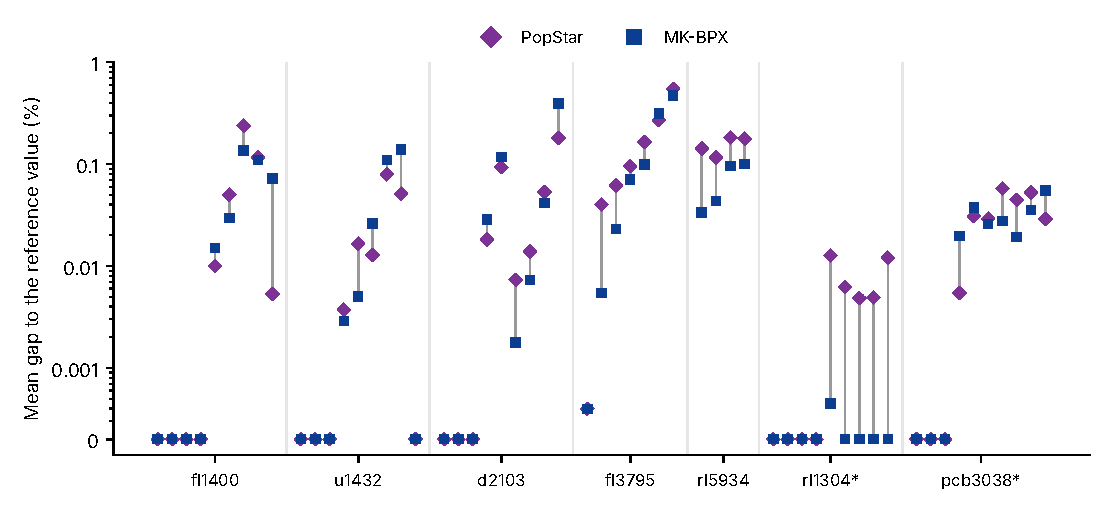
\includegraphics[width=\linewidth]{images/fig_sota_pairs.pdf}
  \caption{Mean gap to the reference value of PopStar and \BPX{} on the 57 TSPLIB-based pairs in the second campaign, grouped by instance and ordered by increasing $p$ within each instance (logarithmic scale; the bottom line corresponds to a mean gap of zero). An asterisk marks the two development instances.}
  \label{fig:sotapairs}
\end{figure}

\begin{figure}[htbp]
  \centering
  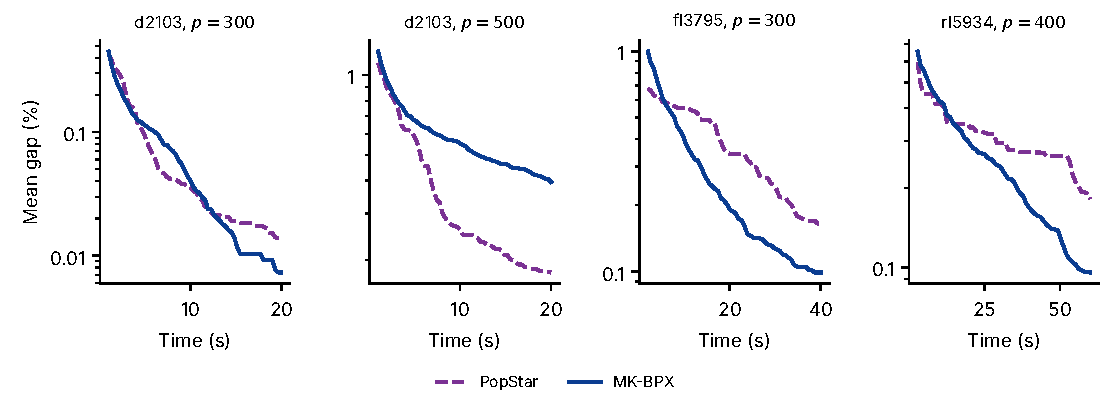
\includegraphics[width=\linewidth]{images/fig_sota_anytime.pdf}
  \caption{Mean gap over the runs as a function of time for PopStar and \BPX{} on the four test pairs of Figure~\ref{fig:anytime}, computed from the improvement traces of the second campaign.}
  \label{fig:sotaanytime}
\end{figure}

\begin{table}[p]
\centering
\caption{Second campaign: results on the three test instances with up to 2103 nodes (10 runs; time limit 10~s, and 20~s for d2103). Gap: mean gap to the reference value $f^*$ in \%. Hits: runs that reached $f^*$ within the time limit. The lower mean gap of each row is in bold when the algorithms differ.}
\label{tab:sotapairs1}
\footnotesize
\setlength{\tabcolsep}{5pt}
\renewcommand{\arraystretch}{0.9}
\begin{tabular}{lrrrrrr}
\toprule
Instance & $p$ & $f^*$ & \multicolumn{2}{c}{PopStar} & \multicolumn{2}{c}{MK-BPX} \\
\cmidrule(lr){4-5}\cmidrule(lr){6-7}
 & & & Gap & Hits & Gap & Hits \\
\midrule
fl1400 & 5 & 174877 & 0.0000 & 10/10 & 0.0000 & 10/10 \\
fl1400 & 10 & 100601 & 0.0000 & 10/10 & 0.0000 & 10/10 \\
fl1400 & 20 & 57191 & 0.0000 & 10/10 & 0.0000 & 10/10 \\
fl1400 & 50 & 28486 & 0.0000 & 10/10 & 0.0000 & 10/10 \\
fl1400 & 100 & 15962 & \textbf{0.0100} & 8/10 & 0.0150 & 7/10 \\
fl1400 & 200 & 8806 & 0.0500 & 0/10 & \textbf{0.0295} & 1/10 \\
fl1400 & 300 & 6109 & 0.2374 & 0/10 & \textbf{0.1359} & 0/10 \\
fl1400 & 400 & 4648 & 0.1162 & 0/10 & \textbf{0.1097} & 0/10 \\
fl1400 & 500 & 3764 & \textbf{0.0053} & 8/10 & 0.0717 & 0/10 \\
\addlinespace[2pt]
u1432 & 5 & 1210126 & 0.0000 & 10/10 & 0.0000 & 10/10 \\
u1432 & 10 & 849759 & 0.0000 & 10/10 & 0.0000 & 10/10 \\
u1432 & 20 & 588766 & 0.0000 & 10/10 & 0.0000 & 10/10 \\
u1432 & 50 & 362072 & 0.0037 & 4/10 & \textbf{0.0029} & 5/10 \\
u1432 & 100 & 243793 & 0.0166 & 1/10 & \textbf{0.0050} & 4/10 \\
u1432 & 200 & 159887 & \textbf{0.0128} & 3/10 & 0.0260 & 0/10 \\
u1432 & 300 & 123689 & \textbf{0.0792} & 0/10 & 0.1094 & 0/10 \\
u1432 & 400 & 103979 & \textbf{0.0513} & 1/10 & 0.1380 & 0/10 \\
u1432 & 500 & 93200 & 0.0000 & 10/10 & 0.0000 & 10/10 \\
\addlinespace[2pt]
d2103 & 5 & 1005136 & 0.0000 & 10/10 & 0.0000 & 10/10 \\
d2103 & 10 & 687321 & 0.0000 & 10/10 & 0.0000 & 10/10 \\
d2103 & 20 & 482926 & 0.0000 & 10/10 & 0.0000 & 10/10 \\
d2103 & 50 & 302190 & \textbf{0.0182} & 0/10 & 0.0286 & 0/10 \\
d2103 & 100 & 194664 & \textbf{0.0931} & 0/10 & 0.1171 & 0/10 \\
d2103 & 200 & 117753 & 0.0073 & 2/10 & \textbf{0.0018} & 7/10 \\
d2103 & 300 & 90471 & 0.0138 & 4/10 & \textbf{0.0073} & 6/10 \\
d2103 & 400 & 75324 & 0.0531 & 0/10 & \textbf{0.0414} & 0/10 \\
d2103 & 500 & 64006 & \textbf{0.1795} & 0/10 & 0.3948 & 0/10 \\
\bottomrule
\end{tabular}
\end{table}

\begin{table}[p]
\centering
\caption{Second campaign: results on the two largest test instances (5 runs; 40~s for fl3795 and 60~s for rl5934) and on the development instances (rl1304: 10 runs, 10~s; pcb3038: 5 runs, 30~s). Columns as in Table~\ref{tab:sotapairs1}. $^{d}$: development instance.}
\label{tab:sotapairs2}
\footnotesize
\setlength{\tabcolsep}{5pt}
\renewcommand{\arraystretch}{0.9}
\begin{tabular}{lrrrrrr}
\toprule
Instance & $p$ & $f^*$ & \multicolumn{2}{c}{PopStar} & \multicolumn{2}{c}{MK-BPX} \\
\cmidrule(lr){4-5}\cmidrule(lr){6-7}
 & & & Gap & Hits & Gap & Hits \\
\midrule
fl3795 & 50 & 150940 & 0.0004 & 4/5 & 0.0004 & 4/5 \\
fl3795 & 100 & 88299 & 0.0401 & 0/5 & \textbf{0.0054} & 1/5 \\
fl3795 & 150 & 65868 & 0.0616 & 0/5 & \textbf{0.0231} & 0/5 \\
fl3795 & 200 & 53928 & 0.0953 & 0/5 & \textbf{0.0708} & 0/5 \\
fl3795 & 300 & 39586 & 0.1652 & 0/5 & \textbf{0.0990} & 0/5 \\
fl3795 & 400 & 31354 & \textbf{0.2698} & 0/5 & 0.3138 & 0/5 \\
fl3795 & 500 & 25976 & 0.5467 & 0/5 & \textbf{0.4689} & 0/5 \\
\addlinespace[2pt]
rl5934 & 200 & 1805530 & 0.1419 & 0/5 & \textbf{0.0335} & 0/5 \\
rl5934 & 300 & 1392419 & 0.1158 & 0/5 & \textbf{0.0434} & 0/5 \\
rl5934 & 400 & 1143940 & 0.1820 & 0/5 & \textbf{0.0956} & 0/5 \\
rl5934 & 500 & 972799 & 0.1774 & 0/5 & \textbf{0.1003} & 0/5 \\
\addlinespace[2pt]
rl1304$^{d}$ & 5 & 3099073 & 0.0000 & 10/10 & 0.0000 & 10/10 \\
rl1304$^{d}$ & 10 & 2134295 & 0.0000 & 10/10 & 0.0000 & 10/10 \\
rl1304$^{d}$ & 20 & 1412108 & 0.0000 & 10/10 & 0.0000 & 10/10 \\
rl1304$^{d}$ & 50 & 795012 & 0.0000 & 10/10 & 0.0000 & 10/10 \\
rl1304$^{d}$ & 100 & 491639 & 0.0127 & 3/10 & \textbf{0.0004} & 9/10 \\
rl1304$^{d}$ & 200 & 268573 & 0.0062 & 5/10 & \textbf{0.0000} & 10/10 \\
rl1304$^{d}$ & 300 & 177326 & 0.0048 & 2/10 & \textbf{0.0000} & 10/10 \\
rl1304$^{d}$ & 400 & 128332 & 0.0049 & 4/10 & \textbf{0.0000} & 10/10 \\
rl1304$^{d}$ & 500 & 97024 & 0.0121 & 1/10 & \textbf{0.0000} & 10/10 \\
\addlinespace[2pt]
pcb3038$^{d}$ & 5 & 1777835 & 0.0000 & 5/5 & 0.0000 & 5/5 \\
pcb3038$^{d}$ & 10 & 1211704 & 0.0000 & 5/5 & 0.0000 & 5/5 \\
pcb3038$^{d}$ & 20 & 839494 & 0.0000 & 5/5 & 0.0000 & 5/5 \\
pcb3038$^{d}$ & 50 & 506339 & \textbf{0.0054} & 4/5 & 0.0196 & 2/5 \\
pcb3038$^{d}$ & 100 & 351500 & \textbf{0.0308} & 0/5 & 0.0376 & 1/5 \\
pcb3038$^{d}$ & 150 & 280128 & 0.0291 & 0/5 & \textbf{0.0257} & 0/5 \\
pcb3038$^{d}$ & 200 & 237399 & 0.0576 & 0/5 & \textbf{0.0276} & 0/5 \\
pcb3038$^{d}$ & 300 & 186833 & 0.0445 & 0/5 & \textbf{0.0193} & 0/5 \\
pcb3038$^{d}$ & 400 & 156276 & 0.0523 & 0/5 & \textbf{0.0356} & 0/5 \\
pcb3038$^{d}$ & 500 & 134798 & \textbf{0.0289} & 0/5 & 0.0549 & 0/5 \\
\bottomrule
\end{tabular}
\end{table}

\paragraph{OR-Library.} On the 40 OR-Library instances both algorithms found the optimum in all \mPORuns{} runs within the time limits, so there is no difference to test and H6 is not rejected (Table~\ref{tab:sotatests}). The optimum was reached after \mPOTtPop\% of the time limit on average by PopStar and after \mPOTtBpx\% by \BPX; PopStar was the faster of the two in \mPOTtPopFaster{} instances. As in Section~\ref{sec:res_orlib}, this benchmark does not discriminate between good heuristics that share a fast local search.

\paragraph{Longer runs.} The experiment of Section~\ref{sec:res_long} was repeated for PopStar and \BPX, again side by side: five runs with five times the time limit on the \mPLPairs{} test pairs with $p\geq100$ and $n\leq2103$ (Table~\ref{tab:sotalong}). On these pairs PopStar has the lower average gap at the original limits (\mPLspopGap\% against \mPLsbpxGap\%; each algorithm better in \mPLsW{} pairs). With five times the limit the order is reversed: the mean gap of PopStar falls to \mPLpopGap\% and that of \BPX{} to \mPLbpxGap\%, a reduction by a factor of \mPLpopImp{} and \mPLbpxImp{} respectively, and \mPLbpxHit\% of the runs of \BPX{} are optimal against \mPLpopHit\% of those of PopStar. \BPX{} has the lower mean gap in \mPLW{} pairs and the higher in \mPLL{} (\mPLLostList), the three pairs with many medians in which PopStar is clearly ahead at both time scales. With 15 pairs the difference is not significant ($P=\mPLP$, descriptive), so these runs do not establish that \BPX{} is better at longer times; they do show that its standing with respect to PopStar does not deteriorate when both are given more time, and that on d2103 and u1432 most of the distance observed at the short limits disappears.

\begin{table}[htbp]
\centering
\caption{PopStar and \BPX{} on the \mPLPairs{} test pairs with $p\geq100$ and $n\leq 2103$: average of the mean gaps (\%) and share of optimal runs (\%). Ten runs with the time limits of Table~\ref{tab:instances} and five runs with five times those limits, both algorithms side by side.}
\label{tab:sotalong}
\small
\setlength{\tabcolsep}{4pt}
\begin{tabular}{lrrrrrrrr}
\toprule
 & \multicolumn{4}{c}{Time limit of Table~\ref{tab:instances}} & \multicolumn{4}{c}{Five times that limit} \\
\cmidrule(lr){2-5}\cmidrule(lr){6-9}
 & \multicolumn{2}{c}{PopStar} & \multicolumn{2}{c}{MK-BPX} & \multicolumn{2}{c}{PopStar} & \multicolumn{2}{c}{MK-BPX} \\
Instance & Gap & Opt.\ (\%) & Gap & Opt.\ (\%) & Gap & Opt.\ (\%) & Gap & Opt.\ (\%) \\
\midrule
fl1400 & 0.0838 & 32 & 0.0724 & 16 & 0.0719 & 40 & 0.0341 & 24 \\
u1432 & 0.0320 & 30 & 0.0557 & 28 & 0.0202 & 48 & 0.0205 & 56 \\
d2103 & 0.0694 & 12 & 0.1125 & 26 & 0.0326 & 24 & 0.0466 & 60 \\
\midrule
All & 0.0617 & 25 & 0.0802 & 23 & 0.0416 & 37 & 0.0338 & 47 \\
\bottomrule
\end{tabular}
\end{table}

\paragraph{Behaviour of PopStar under a time limit.} The number of complete cycles of PopStar per run ranged from \mPopCyclesMin{} to \mPopCyclesMax{} on average over the runs of a pair, depending on its size. Of the improvements of its best solution, \mPopImpMs\% came from the local search that follows the construction, \mPopImpPr\% from path-relinking during the multistart phase and \mPopImpPo\% from post-optimization, so the two intensification mechanisms of the heuristic were fully active under the time limit, and path-relinking found a local minimum inside the path in \mPopPrFound\% of its calls. The overrun of the time limit was the same for the two algorithms (\mPopOver\% of the limit on average for PopStar and \mBpxOver\% for \BPX), and only \mPopLate{} runs of PopStar and \mBpxLate{} of \BPX{} improved their best solution after the limit; these improvements were not counted.

\paragraph{Replication of the main campaign.} The runs of \BPX{} in the second campaign repeat those of the main campaign with the same seeds on another machine of the same type. They performed on average \mRepIter{} times as many iterations (between \mRepIterMin{} and \mRepIterMax{} over the test pairs), so the second machine was slightly faster, and \mRepSameRuns\% of the \mRepRuns{} runs on the test set returned exactly the same value as before. The mean gap of \BPX{} on the test set was \mRepNewGap\% in the second campaign against \mRepMainGap\% in the main one, and the share of optimal runs \mRepNewHit\% against \mRepMainHit\% (Table~\ref{tab:sotatests}, last row). The results of Section~\ref{sec:res_main} are therefore reproduced, and the small systematic shift shows why algorithms that are compared under a time limit must be run on the same machine at the same time.

\subsection{Comparison with the original POPSTAR program}
\label{sec:res_orig}

The third campaign comprises \mXNRunsPop{} runs of POPSTAR and \mXNRunsOurs{} runs of \BPX{} and VNS, made in \mXBlocks{} blocks. Table~\ref{tab:origsummary} aggregates the results, Table~\ref{tab:originst} gives them by instance, Table~\ref{tab:origtests} lists the paired comparisons and Tables~\ref{tab:origpairs1} and~\ref{tab:origpairs2} give the results by pair; Figure~\ref{fig:origpairs} shows the mean gaps side by side and Figure~\ref{fig:origanytime} the gap as a function of time. \mXRefSentence{} Every comparison of this section is made at equal elapsed time (Section~\ref{sec:implementation}).

\paragraph{Published configuration.} With 32 multistart iterations POPSTAR needed between \mXATimeMin{} and \mXATimeMax~s on the TSPLIB-based pairs. On the test pairs this is \mXATTimePct\% of the time limit of Table~\ref{tab:instances} on average (between \mXATTimePctMin\% and \mXATTimePctMax\%); the program is fast on the instances with up to 2103 nodes (\mXANsTimePct\% of the limit) and needs \mXANbTimePct\% of it on the two largest ones, where it exceeded the limit in \mXAOver{} pairs, all of \mXAOverList. At the time used by POPSTAR, the mean gap on the \mXATPairs{} test pairs was \mXATpopGap\% for POPSTAR and \mXATbpxGap\% for \BPX, and \mXATpopHit\% and \mXATbpxHit\% of the runs were at the reference value. \BPX{} had the lower mean gap in \mXATW{} pairs, POPSTAR in \mXATL, and they tied in \mXATT. The mean difference of \mXATSDiff~p.p.\ has a confidence interval that contains zero (95\% CI \mXATCI), and H7 is not rejected ($P=\mHsevenP$; Holm-adjusted $P=\mHsevenPadj$). In the \mXATtPairs{} TSPLIB-based pairs in which every run of both programs reached the reference value, it was reached after \mXATtBpx~s on average by \BPX{} and after \mXATtPop~s by POPSTAR.

\paragraph{Scaled to the time limit.} The number of multistart iterations could be raised in \mXBScaled{} of the 57 TSPLIB-based pairs, to between \mXBKmin{} and \mXBKmax{} iterations, and the scaled runs took \mXBTimePctScaled\% of the time limit on average (\mXBTimePctScaledMin\% to \mXBTimePctScaledMax\%). In the other \mXBNotScaled{} pairs, all of them pairs of the instances with more than 3000 nodes (\mXBNotScaledList), the published configuration leaves no room for more iterations. The additional iterations pay, as the authors of the program indicate: on the \mXBGainPairs{} test pairs that were scaled the mean gap of POPSTAR fell from \mXBGainA\% to \mXBGainB\%, while that of \BPX{} at the corresponding times fell from \mXBGainBpxA\% to \mXBGainBpxB\%. With this configuration the mean gap on the test set was \mXBTpopGap\% for POPSTAR and \mXBTbpxGap\% for \BPX{} (\mXBTpopHit\% and \mXBTbpxHit\% of the runs at the reference value); \BPX{} had the lower mean gap in \mXBTW{} pairs, POPSTAR in \mXBTL, and they tied in \mXBTT. The two mean gaps coincide to four decimal places (95\% CI of the difference \mXBTCI), and H8 is not rejected either ($P=\mHeightP$; Holm-adjusted $P=\mHeightPadj$). Whether POPSTAR is run as published or is given the whole time limit, the data do not separate it from \BPX{} on the test set.

\paragraph{Where each algorithm is ahead.} The aggregate again conceals a pattern, and it is the pattern of the second campaign (Table~\ref{tab:origtests}). On the three test instances with up to 2103 nodes the two programs are level in both configurations (\mXANsW{} pairs for \BPX{} and \mXANsL{} for POPSTAR with the published configuration, $P=\mXANsP$; \mXBNsW{} and \mXBNsL{} with the scaled one, $P=\mXBNsP$), with mean gaps of \mXANspopGap\% for POPSTAR and \mXANsbpxGap\% for \BPX{} in the first case and of \mXBNspopGap\% and \mXBNsbpxGap\% in the second. POPSTAR is clearly the more accurate on the pairs with many medians of these instances, fl1400 with $p=500$, u1432 with $p=300$ and 400 and d2103 with $p=500$, in which relinking distant elite solutions reaches values that kicks around a single solution do not reach in the same time; \BPX{} is ahead on most of the other pairs that are not solved by both. On the two largest instances, fl3795 and rl5934, \BPX{} has the lower mean gap in \mXANbW{} of the \mXANbPairs{} pairs and the higher in \mXANbL{} (mean gap \mXANbbpxGap\% against \mXANbpopGap\% for POPSTAR with the published configuration, $P=\mXANbP$; \mXBNbbpxGap\% against \mXBNbpopGap\% with the scaled one, $P=\mXBNbP$; both descriptive), for the reason given in Section~\ref{sec:res_sota}: within these times POPSTAR completes few multistart iterations, each of which starts from scratch, whereas \BPX{} repairs hundreds of kicks. By number of medians, the two are identical for $p\leq 20$ and close for $p=50$ to 150; \BPX{} has the lower mean gap in \mXBRhiW{} of the \mXBRhiPairs{} test pairs with $p=200$ to 300 (\mXBRhiL{} for POPSTAR), and POPSTAR in \mXBRtopL{} of the \mXBRtopPairs{} pairs with $p\geq 400$ (\mXBRtopW{} for \BPX), with the scaled configuration. The development pairs, reported for completeness, favour \BPX{} (\mXBDbpxGap\% against \mXBDpopGap\%; lower in \mXBDW{} pairs and higher in \mXBDL).

\paragraph{VNS at equal time.} The same blocks contain the runs of VNS on the test instances, which places the control of this study with respect to the state of the art. At the times of the scaled configuration the mean gap of VNS was \mXBTVvnsGap\%, against \mXBTpopGap\% for POPSTAR, which had the lower mean gap in \mXBTVL{} pairs and the higher in \mXBTVW{} ($P=\mXBTVP$, descriptive); with the published configuration the figures are \mXATVvnsGap\% and \mXATpopGap\% (\mXATVL{} pairs against \mXATVW; $P=\mXATVP$). Basic VNS with the local search of this study is thus clearly behind POPSTAR, and the crossover is what closes the distance: \BPX{} had a lower mean gap than VNS in \mXBTCW{} pairs and a higher one in \mXBTCL{} at the same times ($P=\mXBTCP$).

\paragraph{OR-Library.} On the \mXOInst{} OR-Library instances POPSTAR, in its published configuration, took \mXOTimeMean~s on average (\mXOTimePct\% of the time limits of Table~\ref{tab:instances}) and found the optimum in \mXOpopHit\% of its \mXOpopRuns{} runs, with every run optimal in \mXOpopAll{} instances. At the same, very short, times \mXObpxHit\% of the runs of \BPX{} were optimal (every run in \mXObpxAll{} instances), so POPSTAR is marginally ahead there (lower mean gap in \mXAOL{} instances, higher in \mXAOW; $P=\mXAOP$, descriptive), and at the time limits every run of \BPX{} was optimal (\mXObpxHitTl\%). As in Sections~\ref{sec:res_orlib} and~\ref{sec:res_sota}, this benchmark does not discriminate between good heuristics.

\paragraph{Original program and re-implementation.} The third campaign also allows the re-implementation used in Section~\ref{sec:res_sota} to be judged. The two versions of PopStar cannot be set beside each other directly, because the machine of the third campaign was faster than that of the second (see below), but each was measured against \BPX{} on its own machine, at the time limit or close to it. In the second campaign the mean gaps on the test set were \mPTpopGap\% for the re-implementation and \mPTbpxGap\% for \BPX; in the third, \mXBTpopGap\% for the original program scaled to the time limit (which used \mXBTTimePct\% of the limit on average) and \mXBTbpxGap\% for \BPX{} at the same time. \BPX{} had the lower mean gap in \mPTW{} pairs and the higher in \mPTL{} against the re-implementation, and in \mXBTW{} and \mXBTL{} against the original; on the two largest instances the counts are \mPNbW{} and \mPNbL{} against \mXBNbW{} and \mXBNbL. The original program is thus somewhat stronger with respect to \BPX{} than its re-implementation was, mostly on the largest instances, but the difference does not change any conclusion: with either version PopStar and \BPX{} cannot be told apart on the test set, PopStar is ahead on pairs with many medians, and \BPX{} on the largest instances.

\paragraph{Replication of the main results.} The runs of VNS and \BPX{} of the third campaign repeat those of the main campaign with the same seeds. The third machine was faster: the runs completed on average \mXRepBIter{} (\BPX) and \mXRepVIter{} (VNS) times the iterations of the main campaign within the time limits of Table~\ref{tab:instances}, and \mXRepBSame\% and \mXRepVSame\% of them ended at the same value as before. At those limits the mean gap on the test set was \mXHonevnsGap\% for VNS and \mXHonebpxGap\% for \BPX{} (\mXHonevnsHit\% and \mXHonebpxHit\% of optimal runs); \BPX{} had the lower mean gap in \mXHoneW{} pairs and the higher in \mXHoneL{} ($P=\mXHoneP$). The primary result of Section~\ref{sec:res_main} is therefore reproduced on a faster machine, with every pair of runs measured within the same block.

\begin{table}[htbp]
\centering
\caption{Third campaign, the original POPSTAR program against \BPX{} and VNS at equal elapsed time: aggregate results for the two configurations of POPSTAR. Time: mean over the pairs of the elapsed time of POPSTAR, at which the other algorithms are evaluated. Other columns as in Table~\ref{tab:summary}. VNS was run on the test instances only.}
\label{tab:origsummary}
\small
\setlength{\tabcolsep}{4pt}
\resizebox{\textwidth}{!}{\begin{tabular}{lllrrrrrrr}
\toprule
POPSTAR & Set & Algorithm & Pairs & Runs & Time (s) & Mean gap (\%) & Max mean gap (\%) & Optimal runs (\%) & All runs optimal \\
\midrule
Published & Test set & POPSTAR & 38 & 325 & 14.2 & 0.0857 & 0.4250 & 35.4 & 9/38 \\
 &  & MK-BPX & 38 & 325 & 14.2 & 0.0837 & 0.4815 & 37.5 & 11/38 \\
 &  & VNS & 38 & 325 & 14.2 & 0.1868 & 0.7926 & 33.8 & 9/38 \\
\addlinespace[2pt]
 & Test set, $p\geq 100$ & POPSTAR & 25 & 200 & 19.2 & 0.1264 & 0.4250 & 7.5 & 1/25 \\
 &  & MK-BPX & 25 & 200 & 19.2 & 0.1253 & 0.4815 & 7.5 & 1/25 \\
 &  & VNS & 25 & 200 & 19.2 & 0.2794 & 0.7926 & 5.0 & 1/25 \\
\addlinespace[2pt]
 & Development pairs & POPSTAR & 19 & 140 & 10.6 & 0.0260 & 0.0915 & 40.0 & 5/19 \\
 &  & MK-BPX & 19 & 140 & 10.6 & 0.0174 & 0.0758 & 65.0 & 8/19 \\
\addlinespace[2pt]
 & OR-Library & POPSTAR & 40 & 1200 & 0.3 & 0.0005 & 0.0154 & 98.6 & 38/40 \\
 &  & MK-BPX & 40 & 1200 & 0.3 & 0.0008 & 0.0182 & 97.3 & 34/40 \\
\midrule
Scaled & Test set & POPSTAR & 38 & 325 & 21.4 & 0.0562 & 0.4250 & 42.5 & 12/38 \\
 &  & MK-BPX & 38 & 325 & 21.4 & 0.0562 & 0.4435 & 46.8 & 12/38 \\
 &  & VNS & 38 & 325 & 21.4 & 0.1544 & 0.6906 & 35.4 & 11/38 \\
\addlinespace[2pt]
 & Test set, $p\geq 100$ & POPSTAR & 25 & 200 & 25.6 & 0.0843 & 0.4250 & 16.5 & 2/25 \\
 &  & MK-BPX & 25 & 200 & 25.6 & 0.0842 & 0.4435 & 21.0 & 1/25 \\
 &  & VNS & 25 & 200 & 25.6 & 0.2318 & 0.6906 & 6.0 & 1/25 \\
\addlinespace[2pt]
 & Development pairs & POPSTAR & 19 & 140 & 17.7 & 0.0139 & 0.0484 & 55.0 & 7/19 \\
 &  & MK-BPX & 19 & 140 & 17.7 & 0.0108 & 0.0623 & 78.6 & 12/19 \\
\bottomrule
\end{tabular}}
\end{table}

\begin{table}[htbp]
\centering
\caption{Third campaign by instance: average of the mean gaps (\%) at equal elapsed time. Time: elapsed time of POPSTAR as a percentage of the time limit of Table~\ref{tab:instances}; Iter.: multistart iterations of the scaled configuration. $^{d}$: development instance.}
\label{tab:originst}
\small
\setlength{\tabcolsep}{4pt}
\resizebox{\textwidth}{!}{\begin{tabular}{lrrrrrrrrrrr}
\toprule
 & & & \multicolumn{4}{c}{Published configuration} & \multicolumn{5}{c}{Scaled to the time limit} \\
\cmidrule(lr){4-7}\cmidrule(lr){8-12}
Instance & $n$ & Pairs & Time (\%) & POPSTAR & MK-BPX & VNS & Iter. & Time (\%) & POPSTAR & MK-BPX & VNS \\
\midrule
fl1400 & 1400 & 9 & 20 & 0.0772 & 0.0673 & 0.1685 & 208--323 & 87 & 0.0391 & 0.0360 & 0.1369 \\
u1432 & 1432 & 9 & 24 & 0.0424 & 0.0778 & 0.2144 & 111--333 & 85 & 0.0156 & 0.0278 & 0.1542 \\
d2103 & 2103 & 9 & 36 & 0.0791 & 0.0855 & 0.1864 & 84--224 & 86 & 0.0386 & 0.0585 & 0.1486 \\
fl3795 & 3795 & 7 & 64 & 0.1662 & 0.1381 & 0.2414 & 32--124 & 88 & 0.1417 & 0.1279 & 0.2316 \\
rl5934 & 5934 & 4 & 106 & 0.0757 & 0.0349 & 0.0718 & 32 & 106 & 0.0757 & 0.0349 & 0.0718 \\
\midrule
rl1304$^{d}$ & 1304 & 9 & 23 & 0.0112 & 0.0024 & -- & 63--368 & 86 & 0.0029 & 0.0000 & -- \\
pcb3038$^{d}$ & 3038 & 10 & 60 & 0.0394 & 0.0308 & -- & 32--107 & 86 & 0.0238 & 0.0205 & -- \\
\bottomrule
\end{tabular}}
\end{table}

\begin{table}[htbp]
\centering
\caption{Paired comparisons of mean gaps at equal elapsed time in the third campaign. Columns as in Table~\ref{tab:tests}; H7 and H8 are adjusted with Holm's procedure, and the other rows are descriptive.}
\label{tab:origtests}
\small
\setlength{\tabcolsep}{4pt}
\resizebox{\textwidth}{!}{\begin{tabular}{llrrrrrr}
\toprule
Comparison & $x$ vs.\ $y$ & Pairs & $y$ better / worse / tie & Mean diff.\ (p.p.) & 95\% CI & $P$ & Holm $P$ \\
\midrule
\multicolumn{8}{l}{\emph{POPSTAR, published configuration}} \\
\quad H7: test set & POPSTAR vs.\ MK-BPX & 38 & 20 / 9 / 9 & +0.0019 & [-0.0197, +0.0206] & $0.190$ & $0.380$ \\
\quad Test set & POPSTAR vs.\ VNS & 38 & 6 / 25 / 7 & -0.1012 & [-0.1561, -0.0546] & $4.6\times10^{-6}$ & -- \\
\quad Test set & VNS vs.\ MK-BPX & 38 & 29 / 0 / 9 & +0.1031 & [+0.0667, +0.1441] & $3.7\times10^{-9}$ & -- \\
\quad Development pairs & POPSTAR vs.\ MK-BPX & 19 & 12 / 2 / 5 & +0.0087 & [+0.0009, +0.0172] & $0.035$ & -- \\
\quad OR-Library & POPSTAR vs.\ MK-BPX & 40 & 1 / 5 / 34 & -0.0003 & [-0.0011, +0.0003] & $0.312$ & -- \\
\quad Test set, $n\leq 2103$ & POPSTAR vs.\ MK-BPX & 27 & 12 / 6 / 9 & -0.0106 & [-0.0383, +0.0121] & $0.832$ & -- \\
\quad Test set, $n\geq 3795$ & POPSTAR vs.\ MK-BPX & 11 & 8 / 3 / 0 & +0.0327 & [+0.0068, +0.0581] & $0.054$ & -- \\
\quad Test set, $p\leq 20$ & POPSTAR vs.\ MK-BPX & 9 & 2 / 0 / 7 & +0.0001 & [+0.0000, +0.0001] & $0.500$ & -- \\
\quad Test set, $p=50$--$150$ & POPSTAR vs.\ MK-BPX & 9 & 7 / 1 / 1 & +0.0183 & [+0.0057, +0.0323] & $0.039$ & -- \\
\quad Test set, $p=200$--$300$ & POPSTAR vs.\ MK-BPX & 10 & 8 / 2 / 0 & +0.0329 & [-0.0034, +0.0672] & $0.105$ & -- \\
\quad Test set, $p\geq 400$ & POPSTAR vs.\ MK-BPX & 10 & 3 / 6 / 1 & -0.0421 & [-0.1040, +0.0103] & $0.426$ & -- \\
\midrule
\multicolumn{8}{l}{\emph{POPSTAR, scaled to the time limit}} \\
\quad H8: test set & POPSTAR vs.\ MK-BPX & 38 & 16 / 11 / 11 & -0.0000 & [-0.0173, +0.0147] & $0.455$ & $0.455$ \\
\quad Test set & POPSTAR vs.\ VNS & 38 & 2 / 25 / 11 & -0.0982 & [-0.1515, -0.0527] & $1.3\times10^{-6}$ & -- \\
\quad Test set & VNS vs.\ MK-BPX & 38 & 26 / 1 / 11 & +0.0982 & [+0.0588, +0.1429] & $1.0\times10^{-7}$ & -- \\
\quad Development pairs & POPSTAR vs.\ MK-BPX & 19 & 10 / 3 / 6 & +0.0031 & [-0.0011, +0.0073] & $0.191$ & -- \\
\quad Test set, $n\leq 2103$ & POPSTAR vs.\ MK-BPX & 27 & 8 / 8 / 11 & -0.0097 & [-0.0313, +0.0072] & $0.744$ & -- \\
\quad Test set, $n\geq 3795$ & POPSTAR vs.\ MK-BPX & 11 & 8 / 3 / 0 & +0.0236 & [+0.0011, +0.0472] & $0.123$ & -- \\
\quad Test set, $p\leq 20$ & POPSTAR vs.\ MK-BPX & 9 & 0 / 0 / 9 & +0.0000 & [+0.0000, +0.0000] & $1.000$ & -- \\
\quad Test set, $p=50$--$150$ & POPSTAR vs.\ MK-BPX & 9 & 5 / 3 / 1 & +0.0016 & [-0.0114, +0.0136] & $0.742$ & -- \\
\quad Test set, $p=200$--$300$ & POPSTAR vs.\ MK-BPX & 10 & 8 / 2 / 0 & +0.0303 & [+0.0088, +0.0533] & $0.049$ & -- \\
\quad Test set, $p\geq 400$ & POPSTAR vs.\ MK-BPX & 10 & 3 / 6 / 1 & -0.0319 & [-0.0849, +0.0123] & $0.301$ & -- \\
\bottomrule
\end{tabular}}
\end{table}

\begin{figure}[htbp]
  \centering
  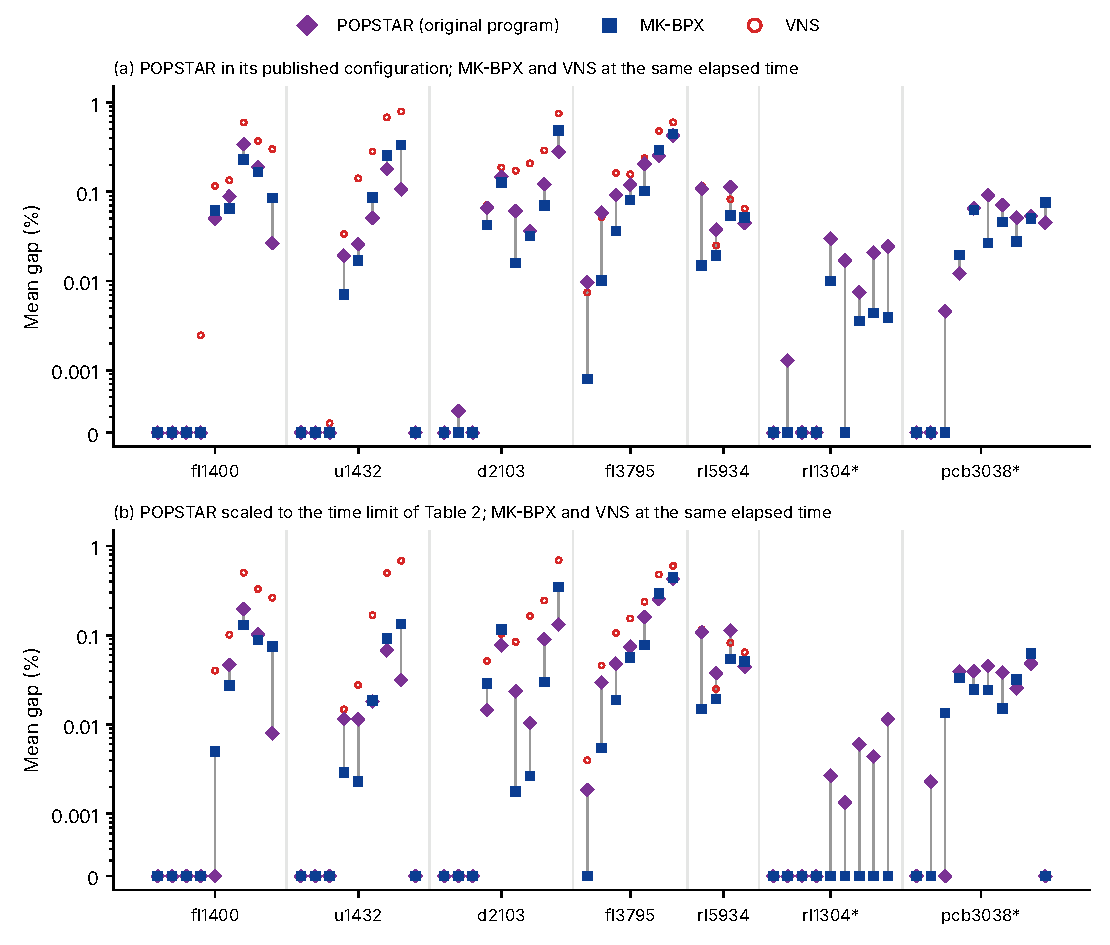
\includegraphics[width=\linewidth]{images/fig_orig_pairs.pdf}
  \caption{Mean gap to the reference value of the original POPSTAR program, \BPX{} and VNS at equal elapsed time on the 57 TSPLIB-based pairs, grouped by instance and ordered by increasing $p$ within each instance (logarithmic scale; the bottom line corresponds to a mean gap of zero). An asterisk marks the two development instances, on which VNS was not run.}
  \label{fig:origpairs}
\end{figure}

\begin{figure}[htbp]
  \centering
  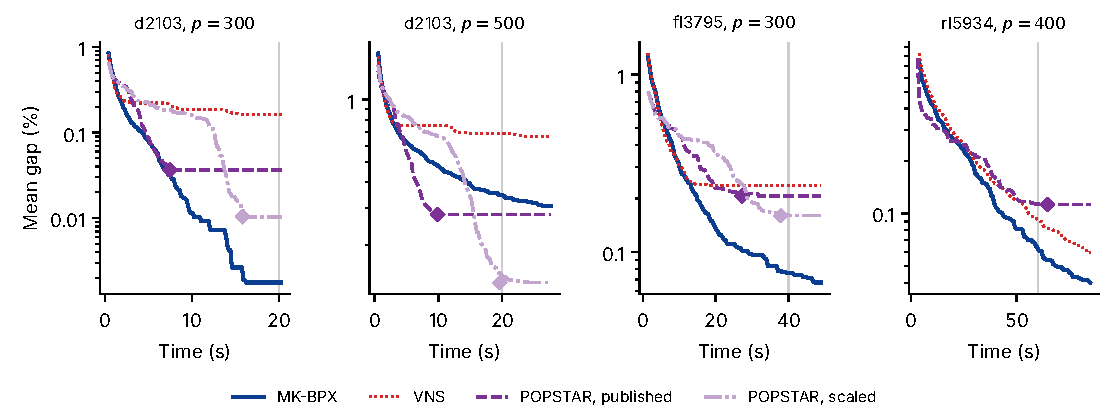
\includegraphics[width=\linewidth]{images/fig_orig_anytime.pdf}
  \caption{Mean gap over the runs as a function of elapsed time in the third campaign, computed from the improvement traces. The curve of a program starts when all its runs have a solution; the diamonds mark the mean time and mean gap at which POPSTAR ends, and the vertical line the time limit of Table~\ref{tab:instances}.}
  \label{fig:origanytime}
\end{figure}

\begin{table}[p]
\centering
\caption{Third campaign: results on the three test instances with up to 2103 nodes (10 runs). $t$: mean elapsed time of POPSTAR, at which \BPX{} is evaluated. Iter.: multistart iterations of the scaled configuration (no entry: the published configuration already uses the time limit). Gap: mean gap to the reference value $f^*$ in \%. Hits: runs that reached $f^*$. The lower mean gap of each comparison is in bold when the algorithms differ.}
\label{tab:origpairs1}
\footnotesize
\setlength{\tabcolsep}{3.5pt}
\renewcommand{\arraystretch}{0.9}
\resizebox{\textwidth}{!}{\begin{tabular}{lrr@{\hskip 10pt}rrrrr@{\hskip 10pt}rrrrrr}
\toprule
 & & & \multicolumn{5}{c}{Published configuration (32 iterations)} & \multicolumn{6}{c}{Scaled to the time limit} \\
\cmidrule(lr){4-8}\cmidrule(lr){9-14}
 & & & & \multicolumn{2}{c}{POPSTAR} & \multicolumn{2}{c}{MK-BPX} & & & \multicolumn{2}{c}{POPSTAR} & \multicolumn{2}{c}{MK-BPX} \\
\cmidrule(lr){5-6}\cmidrule(lr){7-8}\cmidrule(lr){11-12}\cmidrule(lr){13-14}
Instance & $p$ & $f^*$ & $t$ (s) & Gap & Hits & Gap & Hits & Iter. & $t$ (s) & Gap & Hits & Gap & Hits \\
\midrule
fl1400 & 5 & 174877 & 1.4 & 0.0000 & 10/10 & 0.0000 & 10/10 & 209 & 9.1 & 0.0000 & 10/10 & 0.0000 & 10/10 \\
fl1400 & 10 & 100601 & 1.2 & 0.0000 & 10/10 & 0.0000 & 10/10 & 262 & 9.0 & 0.0000 & 10/10 & 0.0000 & 10/10 \\
fl1400 & 20 & 57191 & 1.1 & 0.0000 & 10/10 & 0.0000 & 10/10 & 286 & 9.5 & 0.0000 & 10/10 & 0.0000 & 10/10 \\
fl1400 & 50 & 28486 & 1.4 & 0.0000 & 10/10 & 0.0000 & 10/10 & 277 & 8.3 & 0.0000 & 10/10 & 0.0000 & 10/10 \\
fl1400 & 100 & 15962 & 1.8 & \textbf{0.0501} & 3/10 & 0.0614 & 0/10 & 323 & 8.4 & \textbf{0.0000} & 10/10 & 0.0050 & 9/10 \\
fl1400 & 200 & 8806 & 2.3 & 0.0886 & 0/10 & \textbf{0.0647} & 0/10 & 273 & 9.2 & 0.0466 & 0/10 & \textbf{0.0273} & 1/10 \\
fl1400 & 300 & 6109 & 3.1 & 0.3405 & 0/10 & \textbf{0.2292} & 0/10 & 215 & 8.4 & 0.1964 & 0/10 & \textbf{0.1293} & 0/10 \\
fl1400 & 400 & 4648 & 2.5 & 0.1893 & 0/10 & \textbf{0.1657} & 0/10 & 244 & 9.0 & 0.1011 & 0/10 & \textbf{0.0882} & 0/10 \\
fl1400 & 500 & 3764 & 2.7 & \textbf{0.0266} & 2/10 & 0.0850 & 0/10 & 208 & 7.4 & \textbf{0.0080} & 7/10 & 0.0744 & 0/10 \\
\addlinespace[2pt]
u1432 & 5 & 1210126 & 2.7 & 0.0000 & 10/10 & 0.0000 & 10/10 & 111 & 8.7 & 0.0000 & 10/10 & 0.0000 & 10/10 \\
u1432 & 10 & 849759 & 3.2 & 0.0000 & 10/10 & 0.0000 & 10/10 & 118 & 8.5 & 0.0000 & 10/10 & 0.0000 & 10/10 \\
u1432 & 20 & 588766 & 2.3 & 0.0000 & 10/10 & 0.0000 & 10/10 & 163 & 8.4 & 0.0000 & 10/10 & 0.0000 & 10/10 \\
u1432 & 50 & 362072 & 2.8 & 0.0192 & 1/10 & \textbf{0.0070} & 4/10 & 262 & 8.1 & 0.0115 & 1/10 & \textbf{0.0029} & 5/10 \\
u1432 & 100 & 243793 & 1.9 & 0.0259 & 0/10 & \textbf{0.0171} & 0/10 & 333 & 8.8 & 0.0114 & 0/10 & \textbf{0.0023} & 6/10 \\
u1432 & 200 & 159887 & 2.2 & \textbf{0.0509} & 0/10 & 0.0864 & 0/10 & 300 & 8.8 & \textbf{0.0181} & 1/10 & 0.0186 & 0/10 \\
u1432 & 300 & 123689 & 2.6 & \textbf{0.1793} & 0/10 & 0.2544 & 0/10 & 248 & 8.2 & \textbf{0.0677} & 0/10 & 0.0924 & 0/10 \\
u1432 & 400 & 103979 & 2.6 & \textbf{0.1065} & 0/10 & 0.3352 & 0/10 & 221 & 7.6 & \textbf{0.0315} & 3/10 & 0.1341 & 0/10 \\
u1432 & 500 & 93200 & 1.5 & 0.0000 & 10/10 & 0.0000 & 10/10 & 282 & 9.6 & 0.0000 & 10/10 & 0.0000 & 10/10 \\
\addlinespace[2pt]
d2103 & 5 & 1005136 & 7.0 & 0.0000 & 10/10 & 0.0000 & 10/10 & 84 & 16.6 & 0.0000 & 10/10 & 0.0000 & 10/10 \\
d2103 & 10 & 687321 & 7.4 & 0.0003 & 9/10 & \textbf{0.0000} & 10/10 & 104 & 17.7 & 0.0000 & 10/10 & 0.0000 & 10/10 \\
d2103 & 20 & 482926 & 6.7 & 0.0001 & 7/10 & \textbf{0.0000} & 10/10 & 137 & 15.7 & 0.0000 & 10/10 & 0.0000 & 10/10 \\
d2103 & 50 & 302190 & 6.8 & 0.0660 & 0/10 & \textbf{0.0424} & 0/10 & 172 & 17.2 & \textbf{0.0145} & 0/10 & 0.0286 & 0/10 \\
d2103 & 100 & 194664 & 5.3 & 0.1468 & 0/10 & \textbf{0.1275} & 0/10 & 224 & 16.1 & \textbf{0.0770} & 0/10 & 0.1159 & 0/10 \\
d2103 & 200 & 117753 & 6.1 & 0.0609 & 0/10 & \textbf{0.0160} & 2/10 & 202 & 17.5 & 0.0235 & 2/10 & \textbf{0.0018} & 7/10 \\
d2103 & 300 & 90471 & 7.5 & 0.0363 & 0/10 & \textbf{0.0321} & 1/10 & 173 & 15.8 & 0.0104 & 0/10 & \textbf{0.0027} & 7/10 \\
d2103 & 400 & 75324 & 8.5 & 0.1213 & 0/10 & \textbf{0.0704} & 0/10 & 145 & 19.0 & 0.0904 & 0/10 & \textbf{0.0297} & 0/10 \\
d2103 & 500 & 64006 & 9.9 & \textbf{0.2800} & 0/10 & 0.4815 & 0/10 & 118 & 19.6 & \textbf{0.1316} & 0/10 & 0.3479 & 0/10 \\
\bottomrule
\end{tabular}}
\end{table}

\begin{table}[p]
\centering
\caption{Third campaign: results on the two largest test instances and on the development instances (5 runs; 10 runs for rl1304). Columns as in Table~\ref{tab:origpairs1}. $^{d}$: development instance.}
\label{tab:origpairs2}
\footnotesize
\setlength{\tabcolsep}{3.5pt}
\renewcommand{\arraystretch}{0.9}
\resizebox{\textwidth}{!}{\begin{tabular}{lrr@{\hskip 10pt}rrrrr@{\hskip 10pt}rrrrrr}
\toprule
 & & & \multicolumn{5}{c}{Published configuration (32 iterations)} & \multicolumn{6}{c}{Scaled to the time limit} \\
\cmidrule(lr){4-8}\cmidrule(lr){9-14}
 & & & & \multicolumn{2}{c}{POPSTAR} & \multicolumn{2}{c}{MK-BPX} & & & \multicolumn{2}{c}{POPSTAR} & \multicolumn{2}{c}{MK-BPX} \\
\cmidrule(lr){5-6}\cmidrule(lr){7-8}\cmidrule(lr){11-12}\cmidrule(lr){13-14}
Instance & $p$ & $f^*$ & $t$ (s) & Gap & Hits & Gap & Hits & Iter. & $t$ (s) & Gap & Hits & Gap & Hits \\
\midrule
fl3795 & 50 & 150940 & 16.7 & 0.0097 & 3/5 & \textbf{0.0008} & 3/5 & 124 & 33.8 & 0.0019 & 4/5 & \textbf{0.0000} & 5/5 \\
fl3795 & 100 & 88299 & 22.8 & 0.0582 & 0/5 & \textbf{0.0102} & 1/5 & 92 & 34.3 & 0.0294 & 0/5 & \textbf{0.0054} & 1/5 \\
fl3795 & 150 & 65868 & 21.0 & 0.0917 & 0/5 & \textbf{0.0364} & 0/5 & 102 & 35.1 & 0.0480 & 0/5 & \textbf{0.0188} & 0/5 \\
fl3795 & 200 & 53928 & 24.8 & 0.1198 & 0/5 & \textbf{0.0805} & 0/5 & 77 & 37.3 & 0.0742 & 0/5 & \textbf{0.0560} & 0/5 \\
fl3795 & 300 & 39586 & 27.2 & 0.2056 & 0/5 & \textbf{0.1016} & 0/5 & 60 & 37.9 & 0.1602 & 0/5 & \textbf{0.0778} & 0/5 \\
fl3795 & 400 & 31354 & 33.9 & \textbf{0.2532} & 0/5 & 0.2941 & 0/5 & 32 & 33.9 & \textbf{0.2532} & 0/5 & 0.2941 & 0/5 \\
fl3795 & 500 & 25976 & 33.7 & \textbf{0.4250} & 0/5 & 0.4435 & 0/5 & 32 & 33.7 & \textbf{0.4250} & 0/5 & 0.4435 & 0/5 \\
\addlinespace[2pt]
rl5934 & 200 & 1805530 & 57.3 & 0.1081 & 0/5 & \textbf{0.0148} & 1/5 & 32 & 57.3 & 0.1081 & 0/5 & \textbf{0.0148} & 1/5 \\
rl5934 & 300 & 1392419 & 64.8 & 0.0375 & 0/5 & \textbf{0.0193} & 0/5 & 32 & 64.8 & 0.0375 & 0/5 & \textbf{0.0193} & 0/5 \\
rl5934 & 400 & 1143940 & 64.5 & 0.1127 & 0/5 & \textbf{0.0542} & 0/5 & 32 & 64.5 & 0.1127 & 0/5 & \textbf{0.0542} & 0/5 \\
rl5934 & 500 & 972799 & 68.4 & \textbf{0.0446} & 0/5 & 0.0511 & 0/5 & 32 & 68.4 & \textbf{0.0446} & 0/5 & 0.0511 & 0/5 \\
\addlinespace[2pt]
rl1304$^{d}$ & 5 & 3099073 & 4.7 & 0.0000 & 10/10 & 0.0000 & 10/10 & 63 & 8.7 & 0.0000 & 10/10 & 0.0000 & 10/10 \\
rl1304$^{d}$ & 10 & 2134295 & 4.2 & 0.0013 & 9/10 & \textbf{0.0000} & 10/10 & 88 & 8.4 & 0.0000 & 10/10 & 0.0000 & 10/10 \\
rl1304$^{d}$ & 20 & 1412108 & 2.5 & 0.0000 & 10/10 & 0.0000 & 10/10 & 158 & 8.2 & 0.0000 & 10/10 & 0.0000 & 10/10 \\
rl1304$^{d}$ & 50 & 795012 & 1.3 & 0.0000 & 10/10 & 0.0000 & 10/10 & 331 & 8.9 & 0.0000 & 10/10 & 0.0000 & 10/10 \\
rl1304$^{d}$ & 100 & 491639 & 1.7 & 0.0298 & 0/10 & \textbf{0.0100} & 3/10 & 368 & 8.9 & 0.0027 & 5/10 & \textbf{0.0000} & 10/10 \\
rl1304$^{d}$ & 200 & 268573 & 1.4 & 0.0169 & 1/10 & \textbf{0.0000} & 10/10 & 338 & 8.4 & 0.0013 & 7/10 & \textbf{0.0000} & 10/10 \\
rl1304$^{d}$ & 300 & 177326 & 1.6 & 0.0074 & 2/10 & \textbf{0.0036} & 5/10 & 310 & 8.4 & 0.0060 & 2/10 & \textbf{0.0000} & 10/10 \\
rl1304$^{d}$ & 400 & 128332 & 1.6 & 0.0207 & 1/10 & \textbf{0.0044} & 8/10 & 307 & 8.4 & 0.0044 & 2/10 & \textbf{0.0000} & 10/10 \\
rl1304$^{d}$ & 500 & 97024 & 1.8 & 0.0243 & 0/10 & \textbf{0.0039} & 7/10 & 309 & 8.8 & 0.0114 & 3/10 & \textbf{0.0000} & 10/10 \\
\addlinespace[2pt]
pcb3038$^{d}$ & 5 & 1777835 & 23.6 & 0.0000 & 5/5 & 0.0000 & 5/5 & 32 & 23.6 & 0.0000 & 5/5 & 0.0000 & 5/5 \\
pcb3038$^{d}$ & 10 & 1211704 & 19.6 & 0.0000 & 5/5 & 0.0000 & 5/5 & 51 & 28.8 & 0.0000 & 5/5 & 0.0000 & 5/5 \\
pcb3038$^{d}$ & 20 & 839494 & 20.1 & 0.0046 & 1/5 & \textbf{0.0000} & 5/5 & 56 & 24.4 & 0.0023 & 3/5 & \textbf{0.0000} & 5/5 \\
pcb3038$^{d}$ & 50 & 506339 & 14.6 & \textbf{0.0122} & 2/5 & 0.0196 & 2/5 & 107 & 25.8 & \textbf{0.0000} & 5/5 & 0.0134 & 3/5 \\
pcb3038$^{d}$ & 100 & 351500 & 17.1 & 0.0651 & 0/5 & \textbf{0.0627} & 1/5 & 90 & 27.8 & 0.0393 & 0/5 & \textbf{0.0331} & 1/5 \\
pcb3038$^{d}$ & 150 & 280128 & 15.8 & 0.0915 & 0/5 & \textbf{0.0267} & 0/5 & 93 & 25.2 & 0.0396 & 0/5 & \textbf{0.0247} & 0/5 \\
pcb3038$^{d}$ & 200 & 237399 & 15.7 & 0.0709 & 0/5 & \textbf{0.0457} & 0/5 & 92 & 29.3 & 0.0452 & 0/5 & \textbf{0.0244} & 1/5 \\
pcb3038$^{d}$ & 300 & 186833 & 16.6 & 0.0512 & 0/5 & \textbf{0.0275} & 0/5 & 81 & 23.2 & 0.0381 & 0/5 & \textbf{0.0151} & 0/5 \\
pcb3038$^{d}$ & 400 & 156276 & 17.7 & 0.0536 & 0/5 & \textbf{0.0504} & 0/5 & 70 & 25.6 & \textbf{0.0253} & 0/5 & 0.0321 & 0/5 \\
pcb3038$^{d}$ & 500 & 134798 & 20.6 & \textbf{0.0450} & 0/5 & 0.0758 & 0/5 & 56 & 24.9 & \textbf{0.0484} & 0/5 & 0.0623 & 0/5 \\
\bottomrule
\end{tabular}}
\end{table}

% =====================================================================
\section{Discussion}
\label{sec:discussion}

\paragraph{Why recombining an offspring with its parent helps.}
A kick followed by local search is an experiment carried out simultaneously in several regions of the instance. VNS judges it by its total. BPX judges each region separately and, through the balance constraint, also the transfers of facilities between regions. The experiments confirm the two consequences one would expect. The benefit grows with the number of medians, because more medians mean more and smaller regions and hence more components (Table~\ref{tab:mech}). And the best shaking range changes: a short cycle of small kicks is the better choice for VNS, whereas \BPX{} profits from the full cycle, in which large kicks perturb many regions at once (Table~\ref{tab:dev}). The crossover thus turns a weakness of perturbation-based search on large instances, the low probability that a large perturbation improves the total cost, into a source of improvements.

\paragraph{Position with respect to the state of the art.}
PopStar and \BPX{} are built on the same local search and represent two ways of using it. PopStar samples many independent local optima and intensifies by relinking them through a pool; \BPX{} stays in the neighbourhood of one solution and extracts more from each perturbation. Under equal conditions neither dominates (Section~\ref{sec:res_sota}). \BPX{} matches PopStar on the test set as a whole with a much simpler algorithm, which has no pool, no construction heuristic and no parameter beyond those of basic VNS, and it is the better choice when the time available allows only a few restarts, as on the largest instances; with five times the time limit it also tends to end ahead on the mid-sized ones. PopStar is the better choice on several mid-sized pairs, notably on u1432 and on d2103 with $p=500$, where relinking distant local optima reaches regions that kicks around a single solution do not reach in the same time. The two mechanisms are thus complementary rather than competing: BPX merges solutions that are close, path-relinking connects solutions that are far apart, and the results give a concrete reason to combine them. The comparison with the original program of the authors of PopStar (Section~\ref{sec:res_orig}) confirms this reading with an independent implementation and a different local search: at equal elapsed time neither program dominates, whether POPSTAR is run as published or with the number of iterations that fills the time limit, the pairs on which it is ahead are again mostly those with many medians, and \BPX{} is again ahead on the two largest instances. It also places basic VNS, which with the same local search and the same time is clearly behind POPSTAR; the crossover alone accounts for the distance between a method that is behind the reference heuristic and one that is level with it.

\paragraph{What the population contributes.}
In \BPX{} recombination is essential and the population is minimal. This contrasts with the usual picture of a memetic algorithm and with our earlier design, and the results on the number of elite copies (Section~\ref{sec:res_factors}) suggest that, at the time scales studied, nothing is gained by spreading the effort over several copies of the elite solution that are fused later, since BPX already fuses every offspring as soon as it is produced. BPX requires parents that share most of their facilities; two independent local optima usually form one large component, and the crossover then returns the better parent. Populations of diverse solutions therefore need a different operator, such as path-relinking, and combining the two is a natural extension: path-relinking to move between distant elite solutions, BPX to merge solutions that are close.

\paragraph{Scope of the operator.}
BPX uses only two properties of the $p$MP: every customer is served by its closest open facility, and the number of facilities is fixed. The first gives Proposition~\ref{prop:bound}; the second gives the selection problem. The same construction applies, with a different constraint or none, to related problems. For the uncapacitated facility location problem the components carry the fixed costs of their facilities and can be chosen independently, so the selection is trivial; for the $p$-centre and for capacitated variants the bound would have to be adapted. BPX is also independent of the local search and of the way the second parent is produced, and could be added to other heuristics for the $p$MP that generate neighbouring local optima.

\paragraph{Threats to validity.}
\emph{Internal validity.} VNS and \BPX{} share all their code and differ in one switch, so the comparison isolates the crossover; the tuned control \VNSs{} addresses the possibility that the shaking range favours \BPX. Other variants of VNS and other acceptance rules were not implemented. The kick schedule of \BPX{} was taken from VNS and not tuned beyond the three ranges of Table~\ref{tab:dev}. The larger instances were run five times and with time limits that allow only a few hundred iterations, so the results on them describe the early phase of the search. Times were measured on a shared virtual machine, which adds noise to individual timings; all runs were executed under the same load, two processes on two cores, and those of VNS and \BPX{} side by side on the same pairs, so the noise affects them equally. Finally, the pairs derived from one instance are not independent observations. At the level of the instance, \BPX{} had the lower average gap on each of the \mInstN{} TSPLIB instances, the five test instances and the two development ones (two-sided sign test $P=\mInstP$).

\emph{External validity.} The test set contains five TSPLIB-based instances with Euclidean distances and the OR-Library instances are random graphs; instances with other structures, such as the RW instances with random distance matrices \citep{resende_hybrid_2004}, in which regions are not localized, were not considered, and the decomposition may be less effective on them. The largest instance has 5934 nodes; the quadratic memory of the distance matrix and of the sorted lists limits the present implementation to instances of this order.

\emph{Construct validity.} The comparison with the state of the art rests on two experiments, each of which covers the weakness of the other. The re-implementation of PopStar (Section~\ref{sec:res_sota}) equalizes the language, the local search and the clock, so that only the search strategies differ, but it may deviate from the original in details that the published description leaves open, such as tie-breaking and the exact rule that ends the post-optimization; its path-relinking was verified against brute force and its results with the published settings agree with the published ones, which bounds this risk without removing it. The original program (Section~\ref{sec:res_orig}) removes that doubt, but it compares complete systems: POPSTAR is compiled C++ whose local search updates the gain, loss and extra structures incrementally between moves, whereas \BPX{} is compiled from Python by Numba and recomputes them in every scan with distance-ordered lists, so a difference between the two could be due to the implementation as much as to the algorithm. That the two experiments lead to the same conclusions makes neither explanation likely. The original program has no time limit; it was compared at equal elapsed time with its number of iterations as the only parameter changed, its elapsed time was measured from outside the program, and stopping \BPX{} at the moment at which POPSTAR happens to end is not how either would be used in practice, which is why the values at the time limits are reported as well. All timings come from shared virtual machines whose speed drifts by 10 to 20\% over hours; pinned processes, the repetition of disturbed runs and, in the third campaign, blocks that contain all the runs of a pair limit this threat, and the fixed computation timed inside the blocks varied by \mXOracleIn\% on average. PopStar was run with its default parameters, confirmed on the development pairs for the re-implementation, and neither it nor \BPX{} was tuned further. Other strong heuristics for the $p$MP, among them the population-based search of \citet{pullan_population_2008} and variable neighbourhood decomposition search \citep{hansen_vns_2001}, were not included. The claims of this paper are therefore two: adding BPX to a perturbation-based search improves it significantly at no extra cost, and the resulting algorithm is on a par with PopStar, re-implemented or original, under the conditions studied, without being shown superior to it.

% =====================================================================
\section{Conclusions}
\label{sec:conclusion}

This paper introduced the balanced partition crossover for the $p$-median problem. The operator decomposes the difference between two solutions into components defined by the customers they exchange, bounds the cost of every child that inherits each component from one parent, and selects by dynamic programming the components that minimize the bound while keeping exactly $p$ facilities, so that the child is never worse than either parent. Its cost is linear in the number of customers and it has no parameter. Used to recombine every kicked and re-optimized solution with the solution it came from, it yields a multi-kick memetic algorithm, \BPX, that differs from basic VNS only in the crossover. On \mTPairs{} test pairs with up to 5934 nodes, \BPX{} reduced the mean gap of VNS from \mTvnsGap\% to \mTbpxGap\% in the same time and raised the share of optimal runs from \mTvnsHit\% to \mTbpxHit\%; it was better in \mTW{} pairs and worse in \mTL. It also outperformed a VNS with a tuned shaking range, and reached the optimum in all 1200 runs on the 40 OR-Library instances. The crossover found a usable selection in fewer than 1\% of its calls, yet produced \mBpxSharePct\% of the improvements, and its benefit was largest on instances with many medians. Run side by side with a re-implementation of PopStar that shares its local search, \BPX{} was statistically indistinguishable from it on the test set (mean gap \mPTbpxGap\% against \mPTpopGap\%; lower in \mPTW{} pairs and higher in \mPTL) and more accurate on the two largest instances, while PopStar was more accurate on several mid-sized pairs. The original program of the authors of PopStar, run on the same machine in a design blocked by instance and compared at equal elapsed time, gave the same picture: with its number of iterations scaled to the time limit its mean gap on the test set was \mXBTpopGap\% against \mXBTbpxGap\% for \BPX{} ($P=\mHeightP$), and with its published configuration \mXATpopGap\% against \mXATbpxGap\% ($P=\mHsevenP$), while basic VNS was far behind both. A single solution, a kick and a parameter-free crossover are thus enough to match a pool-based hybrid that has been the reference for the problem for two decades.

Future work includes the combination of BPX with path-relinking in a population of diverse elite solutions, which the comparison with PopStar suggests would join the strengths of both, a comparison with further heuristics, kick schedules designed for BPX rather than inherited from VNS, an implementation with sparse neighbour lists for instances with tens of thousands of nodes, and the extension of the operator to the uncapacitated facility location problem and to capacitated variants.

\section*{Data and code availability}
The implementation, the scripts of the experimental campaign, the run-level logs of all runs (seeds, objective values, counters, times and improvement traces) and the scripts that generate every number, table and figure of Section~\ref{sec:results}, together with the re-implementation of PopStar, its verification, the logs of the second and third campaigns, the exact replay of the main campaign and the scripts that download, compile and run the original POPSTAR program (which belongs to its authors and is not redistributed), are provided as supplementary material and will be released in the repository of the project, \url{https://github.com/ferminriv20/HGA-EBMKI}.

\bibliographystyle{apalike}
\bibliography{references}

\end{document}
